% 感悟论语
% A reading edition set with XeLaTeX.
% Chinese: Noto Serif CJK (Source Han Serif). Latin: TeX Gyre Pagella.
% Quotations: AR PL UKai.
\documentclass[UTF8,fontset=none,openany,twoside,11pt]{ctexbook}

\synctex=1

\usepackage{geometry}
\geometry{
  paperwidth=170mm,
  paperheight=240mm,
  inner=22mm,
  outer=17mm,
  top=19mm,
  bottom=17mm,
  headheight=16pt,
  headsep=6.5mm,
  footskip=11mm,
}

\usepackage{fontspec}
\setmainfont{TeX Gyre Pagella}[
  Scale=0.93,
  Numbers=OldStyle,
  Ligatures=TeX,
]
\setCJKmainfont{Noto Serif CJK SC}[
  BoldFont={Noto Serif CJK SC Medium},
  ItalicFont={Noto Serif CJK SC},
]
\setCJKsansfont{Noto Sans CJK SC}[
  BoldFont={Noto Sans CJK SC Medium},
]
\setCJKfamilyfont{zhsong}{Noto Serif CJK SC}[
  BoldFont={Noto Serif CJK SC Medium},
]
\setCJKfamilyfont{zhkai}{AR PL UKai CN}
\newcommand{\songti}{\CJKfamily{zhsong}}
\newcommand{\kaishu}{\CJKfamily{zhkai}}

\usepackage{graphicx}
\usepackage{xcolor}
\usepackage{tikz}
\usepackage{enumitem}
\usepackage{fancyhdr}
\usepackage{etoolbox}
\usepackage[most]{tcolorbox}
\usepackage{hyperref}
\usepackage{bookmark}

\definecolor{paper}{HTML}{F7F4EE}
\definecolor{coverbg}{HTML}{E8DCC8}
\definecolor{ink}{HTML}{241F1C}
\definecolor{inksoft}{HTML}{5E584F}
\definecolor{cinnabar}{HTML}{8C3A32}
\definecolor{rule}{HTML}{C9BCAA}
\definecolor{quotebg}{HTML}{F1EBE1}

\pagecolor{paper}
\color{ink}

\linespread{1.28}
\setlength{\parindent}{2em}
\emergencystretch=2.5em
\raggedbottom
\clubpenalty=4000
\widowpenalty=4000

\hypersetup{
  colorlinks=true,
  linkcolor=ink,
  urlcolor=cinnabar,
  citecolor=ink,
  pdftitle={感悟论语：传统文化对现代生活的启示},
  pdfauthor={田冀焕},
  pdfdisplaydoctitle=true,
  bookmarksnumbered=false,
}

% ---------------------------------------------------------------------------
% Plants, part openers, chapter plates
% ---------------------------------------------------------------------------
\newcommand{\thisplant}{artwork/pine.png}
\newcommand{\plantcaption}{}
\newcommand{\partquotetext}{}
\newcommand{\partquotesrc}{}
\newcommand{\currentpartname}{}
\newcommand{\setpartplant}[5]{%
  \renewcommand{\thisplant}{#1}%
  \renewcommand{\plantcaption}{#2}%
  \renewcommand{\partquotetext}{#3}%
  \renewcommand{\partquotesrc}{#4}%
  \renewcommand{\currentpartname}{#5}%
}

\newcommand{\PartNumeral}{%
  \ifcase\value{part}\or 壹\or 贰\or 叁\or 肆\or 伍\or 陆\or 柒\or 捌\or 玖\fi
}

\newif\ifshowchapterplate
\showchapterplatetrue

\newcommand{\chaptertitlefont}[1]{%
  \ifshowchapterplate
    \ifx\currentpartname\@empty\else
      {\zihao{-4}\color{cinnabar}\songti\currentpartname}\par\vspace{2.2mm}%
    \fi
  \fi
  {\zihao{1}\songti\color{ink}#1}%
}

\newcommand{\chapterafter}{%
  \par\vspace{1.6mm}{\color{cinnabar}\rule{14mm}{0.4pt}}%
}

\newcommand{\parttitlefont}[1]{{\zihao{1}\songti\color{ink}#1}}

\newcommand{\partafter}{%
  \par\vspace{5mm}%
  {\color{cinnabar}\rule{14mm}{0.4pt}}\par
  \vspace{7mm}%
  \includegraphics[width=62mm,height=74mm,keepaspectratio]{\thisplant}\par
  \vspace{1.6mm}%
  {\zihao{6}\color{inksoft}\songti\plantcaption}\par
  \ifx\partquotetext\@empty\else
    \vspace{6.5mm}%
    {\zihao{4}\kaishu\color{ink}\partquotetext}\par
    \vspace{1.4mm}%
    {\zihao{-5}\color{cinnabar}\partquotesrc}\par
  \fi
}

\ctexset{
  part = {
    pagestyle = empty,
    numbering = true,
    name = {},
    number = \PartNumeral,
    aftername = \par\vspace{2.2mm},
    format = \centering,
    numberformat = \zihao{-2}\color{cinnabar}\songti,
    titleformat = \parttitlefont,
    aftertitle = \partafter,
    beforeskip = 8mm,
    afterskip = 0pt,
    fixskip = true,
  },
  chapter = {
    pagestyle = plain,
    numbering = false,
    name = {},
    format = \centering,
    titleformat = \chaptertitlefont,
    aftertitle = \chapterafter,
    beforeskip = 8mm,
    afterskip = 8mm,
    fixskip = true,
    afterindent = true,
  },
  section = {
    numbering = false,
    format = \zihao{-3}\songti\raggedright\color{ink},
    beforeskip = 1.35em,
    afterskip = 0.55em,
    fixskip = true,
    afterindent = true,
  },
  subsection = {
    numbering = false,
    format = \zihao{4}\songti\raggedright\color{ink},
    beforeskip = 1em,
    afterskip = 0.4em,
  },
}

% ---------------------------------------------------------------------------
% Running headers and page numbers
% ---------------------------------------------------------------------------
\pagestyle{fancy}
\fancyhf{}
\fancyhead[LE]{\zihao{-5}\color{inksoft}\songti 感悟论语}
\fancyhead[RO]{\zihao{-5}\color{inksoft}\songti\leftmark}
\fancyfoot[LE]{\zihao{-5}\color{inksoft}·\,\thepage\,·}
\fancyfoot[RO]{\zihao{-5}\color{inksoft}·\,\thepage\,·}
\renewcommand{\headrule}{%
  {\color{rule}\hrule height 0.28pt width \headwidth}%
}
\renewcommand{\footrulewidth}{0pt}
\renewcommand{\chaptermark}[1]{\markboth{#1}{}}
\renewcommand{\sectionmark}[1]{}

\fancypagestyle{plain}{%
  \fancyhf{}%
  \fancyfoot[LE,RO]{\zihao{-5}\color{inksoft}·\,\thepage\,·}%
  \renewcommand{\headrulewidth}{0pt}%
  \renewcommand{\headrule}{}%
}

% ---------------------------------------------------------------------------
% Quotations, dates, captions
% ---------------------------------------------------------------------------
\newtcolorbox{classic}{
  breakable,
  enhanced,
  colback=quotebg,
  colframe=quotebg,
  boxrule=0pt,
  arc=0pt,
  outer arc=0pt,
  borderline west={1.15pt}{0pt}{cinnabar},
  left=1.05em,
  right=0.7em,
  top=0.5em,
  bottom=0.45em,
  before skip=0.85em,
  after skip=0.8em,
  fontupper=\kaishu\zihao{5}\color{ink},
  before upper={\parindent=0pt\parskip=0.38em\linespread{1.18}\selectfont},
}

\newcommand{\quotsource}[1]{%
  \par\addvspace{0.75em}%
  {\centering\zihao{5}\kaishu\color{cinnabar}#1\par}%
  \addvspace{0.15em}%
}

\newcommand{\entrydate}[1]{%
  \par\nopagebreak\vspace{0.2em}%
  {\raggedleft\zihao{5}\color{inksoft}#1\par}%
}

\newcommand{\captiontext}{\zihao{6}\kaishu\color{inksoft}}
% A Chinese two-inch portrait is 35 mm by 49 mm.
\newcommand{\discipleportrait}[2]{%
  \par\addvspace{0.55em}%
  \noindent
  \begin{minipage}[t]{36mm}
    \vspace{0pt}%
    \centering
    \includegraphics[width=35mm,height=49mm,keepaspectratio]{#1}%
  \end{minipage}%
  \hspace{3.2mm}%
  \begin{minipage}[t]{\dimexpr\linewidth-36mm-3.2mm\relax}
    \vspace{0pt}%
    \zihao{-5}\songti\color{ink}\raggedright #2%
  \end{minipage}%
  \par\addvspace{0.75em}%
}

\setlist[itemize]{
  leftmargin=1.7em,
  itemsep=0.2em,
  topsep=0.35em,
  parsep=0.05em,
  label=\textcolor{cinnabar}{\textbullet},
}

\pretocmd{\tableofcontents}{\showchapterplatefalse}{}{}
\apptocmd{\tableofcontents}{\showchapterplatetrue}{}{}

% ---------------------------------------------------------------------------
% Cover, title page, colophon, plates
% ---------------------------------------------------------------------------
\newcommand{\coverframe}{%
  \begin{tikzpicture}[remember picture, overlay]
    \draw[cinnabar, line width=0.45pt]
      ([xshift=11mm, yshift=-11mm]current page.north west)
      rectangle
      ([xshift=-11mm, yshift=11mm]current page.south east);
    \draw[ink, line width=0.18pt]
      ([xshift=12.3mm, yshift=-12.3mm]current page.north west)
      rectangle
      ([xshift=-12.3mm, yshift=12.3mm]current page.south east);
  \end{tikzpicture}%
}

\newcommand{\makecover}{%
  \pagecolor{coverbg}%
  \thispagestyle{empty}%
  \coverframe
  \vspace*{0pt plus 1.05fil}%
  \begin{center}
    {\zihao{0}\color{ink}\songti 感悟论语}\\[4mm]
    {\color{cinnabar}\rule{22mm}{0.45pt}}\\[4.2mm]
    {\zihao{4}\color{inksoft}\songti 传统文化对现代生活的启示}\\[13mm]
    {\zihao{-3}\color{ink}\songti 田冀焕}\\[8mm]
    {\zihao{-5}\color{inksoft}\songti 二〇二五}%
  \end{center}
  \vspace*{0pt plus 1.4fil}%
  \clearpage
  \pagecolor{paper}%
}

\newcommand{\makecolophon}{%
  \thispagestyle{empty}%
  \vspace*{18mm}
  \begin{center}
    {\zihao{-3}\songti 感悟论语}\\[1.4mm]
    {\zihao{5}\color{inksoft}\songti 传统文化对现代生活的启示}\\[5mm]
    {\zihao{-4}\songti 田冀焕\ 著}
  \end{center}
  \vspace{8mm}
  \begingroup
    \zihao{5}\songti\color{inksoft}%
    \setlength{\parindent}{0pt}%
    \setlength{\parskip}{0.55em}%
    \setlength{\leftskip}{1.6em}%
    \setlength{\rightskip}{1.6em}%
    本书由作者刊于个人博客「止于至善」（\href{https://jihuan-tian.github.io/}{https://jihuan-tian.github.io/}）的文章整理而成，更新于二〇二五年十月一日。欢迎下载与阅读。本书采用知识共享署名-非商业性使用-禁止演绎\,4.0\,国际许可协议，不得修改，亦不得用于商业目的。\par
    正文汉字用思源宋体（Noto Serif CJK，SIL Open Font License），西文用 \mbox{TeX Gyre Pagella}（GUST Font License）。引文用文鼎\,PL\,简中楷（AR PL UKai，Arphic Public License）。三者都可自由使用。\par
    各卷卷首的松、竹、梅，取岁寒之象，并系于《论语》成句。桃、荇菜、唐棣、木瓜则来自《论语》引及或再三称道的《诗经》。\par
  \endgroup
}

\newcommand{\plate}[3]{%
  \clearpage
  \thispagestyle{empty}%
  \vspace*{6mm}
  \begin{center}
    \includegraphics[width=\textwidth,height=0.74\textheight,keepaspectratio]{#1}\\[5.5mm]
    {\zihao{5}\kaishu\color{inksoft} #2}\\[1.3mm]
    {\zihao{6}\color{cinnabar} #3}
  \end{center}
  \vfill
}

\newcommand{\makeendpage}{%
  \clearpage
  \pagecolor{coverbg}%
  \thispagestyle{empty}%
  \coverframe
  \vspace*{0pt plus 1.05fil}%
  \begin{center}
    {\zihao{-2}\kaishu\color{ink} 学而时习之，不亦说乎}\\[4mm]
    {\color{cinnabar}\rule{22mm}{0.45pt}}\\[4.2mm]
    {\zihao{5}\color{cinnabar}\songti 《论语·学而》}%
  \end{center}
  \vspace*{0pt plus 1.4fil}%
}

\makeatletter
\newcommand{\startfront}{%
  \@mainmatterfalse
  \pagenumbering{roman}%
}
\makeatother

\begin{document}
\startfront
\makecover
\makecolophon
\plate{figures/confucius.png}{明代《孔子燕居像》}{}
\plate{figures/stone-analects.jpg}{学而时习之，不亦说乎}{《论语·学而》}
\renewcommand{\currentpartname}{}
\renewcommand{\thisplant}{artwork/pine.png}
% 卷首.tex
% Auto-generated from 感悟论语.odt by tools/odt_to_tex.py

\chapter{作者简介}

本书作者田冀焕于 2000 年考入清华大学电机系，在此完成了本科学业、博士与博士后的研究工作。爱好传统文化，坚持践行论语的基本观点与思想。目前，作者独立从事高性能数值算法的理论研究与软件开发工作，是开源软件项目 HierBEM 的项目负责人。

\chapter{前言}

我在清华本科期间曾加入旨在弘扬中国传统文化的钟铎社。那时的下午课后，我常与同学在十食堂西侧的小树林内一起朗读朱熹的《四书章句集注》，因而对论语略有涉猎。不过，我当时的阅读与学习并不系统，理解浮于表面、难有心得，更不用说在生活中贯彻践行了。直至2015年，我有幸聆听了傅佩荣老师的《论语300讲》，才算是对论语有了全面的了解和一定的体会。通过持续的学习与践行，我不仅在待人接物方面从中获益匪浅，更是促成了对个人人生方向的探索与逐渐明晰，以及对此方向坚韧不拔的坚守与追寻。

目前市面上常见的与论语相关的书籍大多是针对原文的注释与解读，而展现论语与现代日常生活各方面的诸多关联，以及讲述如何具体应用与践行论语基本原则的书籍较少。本书分享我在学习、科研、职场工作中与论语深度互动、学而时习的体会感悟、心路历程，希望“以文会友，以友辅仁”，向广大读者提供“与孔子对话”的阅读体验，给人生带来启发与积极向上的推动作用。目标读者群主要是对传统文化有兴趣、并希望通过传统文化改善与提升自己的认知与境界的科研工作者、学者、学生、普通读者以及职场人。

目前书稿篇幅约九万余字，包括修养、科研、职场、习惯、家庭、社会、论语解读七部分。每篇文章独立成章，既可连续阅读，也能随手翻阅。此外，在附录中整理了论语章句分类以及孔子与弟子的对话，方便读者系统查阅。

\tableofcontents
\mainmatter
% 品性与修养.tex
% Auto-generated from 感悟论语.odt by tools/odt_to_tex.py

\setpartplant{artwork/pine.png}
  {松柏}
  {岁寒，然后知松柏之后凋也。}
  {《论语·子罕》}
  {品性与修养}
\part{品性与修养}

\chapter{君子品性与儒家精神}

君子不拘泥于表面的嘘寒问暖，他们关注的是在追求至善道路上的慎思笃行。君子自强不息、思想与精神独立，靠的不是相濡以沫、弹冠相庆，而是相望于江湖、各守善道，享一份“有朋自远方来”的乐处便好。尽管“人不己知”，亦不会有愠色，甚至还能激发出“患其不能”的无穷动力。因为深切明白“可与共学，未可与适道；可与适道，未可与立；可与立，未可与权”的道理，即便知音难觅，鲜有人可与碰撞出思想的火花，也同样不忧不惧。君子不担心饮食是否精美、衣着是否时尚、出行是否排场，因为一箪食、一瓢饮便足以支持其终生学习和对真理的追求。由这样的品性，便自然联想到我先前总结的儒家精神。在此重提，以警醒自我：

真正的儒家，有止于至善的终极目标，有君子固穷的气节。既有危邦不入、乱邦不居的小心慬慎，又有可以仕而仕的智慧敏锐。能于箪食瓢饮之间体味人生乐趣，亦有风乎舞雩、歌咏而归的豁达情怀。因为心怀至善而宽容，因为有原则而不妥协。终生学习，以博学、明辨、审问、笃行为乐，以巧言令色、浅尝辄止为耻。

\begin{classic}
《论语·学而篇第一 1.1》 子曰：「学而时习之，不亦说乎？有朋自远方来，不亦乐乎？人不知而不愠，不亦君子乎？」

《论语·宪问篇第十四 14.30》 子曰：「不患人之不己知，患其不能也。」

《论语·子罕篇第九 9.30》 子曰：「可与共学，未可与适道；可与适道，未可与立；可与立，未可与权。」

《论语·颜渊篇第十二 12.4》 司马牛问君子。子曰：「君子不忧不惧。」曰：「不忧不惧，斯谓之君子矣乎？」子曰：「内省不疚，夫何忧何惧？」

《论语·雍也篇第六 6.11》 子曰：「贤哉，回也！一箪食，一瓢饮，在陋巷，人不堪其忧，回也不改其乐。贤哉，回也！」

《论语·卫灵公篇第十五 15.2》 在陈绝粮。从者病，莫能兴。子路愠见曰：「君子亦有穷乎？」子曰：「君子固穷，小人穷斯滥矣。」

《论语·泰伯篇第八 8.13》 子曰：「笃信好学，守死善道。危邦不入，乱邦不居，天下有道则见，无道则隐。邦有道，贫且贱焉，耻也，邦无道，富且贵焉，耻也。」

《论语·先进篇第十一 11.26》 子路、曾皙、冉有、公西华侍坐。子曰：「以吾一日长乎尔，毋吾以也。居则曰：「不吾知也！」如或知尔，则何以哉？」子路率尔而对曰：「千乘之国，摄乎大国之间，加之以师旅，因之以饥馑，由也为之，比及三年，可使有勇，且知方也。」夫子哂之。「求，尔何如？」对曰：「方六七十，如五六十，求也为之，比及三年，可使足民；如其礼乐，以俟君子。」「赤，尔何如？」对曰：「非曰能之，愿学焉！宗庙之事，如会同，端章甫，愿为小相焉。」「点，尔何如？」鼓瑟希，铿尔，舍瑟而作。对曰：「异乎三子者之撰。」子曰：「何伤乎？亦各言其志也。」曰：「莫春者，春服既成；冠者五六人，童子六七人，浴乎沂，风乎舞雩，咏而归。」夫子喟然叹曰：「吾与点也！」三子者出，曾皙后。曾皙曰：「夫三子者之言何如？」子曰：「亦各言其志也已矣！」曰：「夫子何哂由也？」曰：「为国以礼，其言不让，是故哂之。」「唯求则非邦也与？」「安见方六七十，如五六十，而非邦也者。」「唯赤，非邦也与？」「宗庙会同，非诸侯而何？赤也为之小，孰能为之大！」

《论语·颜渊篇第十二 12.15》 子曰：「博学于文，约之以礼，亦可以弗畔矣夫。」

《论语·阳货篇第十七 17.17》 子曰：「巧言令色鲜矣仁。」
\end{classic}

\quotsource{《礼记 儒行》}

\begin{classic}
儒有席上之珍以待聘 ，夙夜强学以待问 ，怀忠信以待举 ，力行以待取 。其自立有如此者 。

儒有可亲而不可劫也 ，可近而不可迫也 ，可杀而不可辱也 。其居处不淫 ，其饮食不溽 ，其过失可微辨而不可面数也 。其刚毅有如此者 。

儒有今人与居，古人与稽，今世行之，后世以为楷。适弗逢世，上弗援，下弗推，谗谄之民有比党而危之者，身可危也，而志不可夺也。虽危，起居竟信其志，犹将不忘百姓之病也。其忧思有如此者。

儒有博学而不穷，笃行而不倦，幽居而不淫，上通而不困。礼之以和为贵，忠信之美，优游之法，慕贤而容众，毁方而瓦合。其宽裕有如此者。

儒有闻善以相告也，见善以相示也，爵位相先也，患难相死也，久相待也，远相致也。其任举有如此者。

儒有澡身而浴德，陈言而伏，静而正之。上弗知也，麤而翘之，又不急为也。不临深而为高，不加少而为多。世治不轻，世乱不沮，同弗与，异弗非也。其特立独行有如此者。

温良者，仁之本也;敬慎者，仁之地也;宽裕者，仁之作也;孙接者，仁之能也;礼节者，仁之貌也;言谈者，仁之文也;歌乐者，仁之和也;分散者，仁之施也。儒皆兼此而有之，犹且不敢言仁也。其尊让有如此者。
\end{classic}

\entrydate{2017.07.27}

\chapter{梁启超《论君子》注释}

君子二字其意甚广，欲为之诠注，颇难得其确解。为英人所称劲德尔门（gentleman）包罗众义，与我国君子之意差相吻合。证之古史，君子每与小人对待【《论语·里仁第四 4.16》子曰：“君子喻于义，小人喻于利。”《论语·述而第七 7.37》子曰：“君子坦荡荡，小人长戚戚。”《论语·卫灵公篇第十五 15.2》 在陈绝粮。从者病，莫能兴。子路愠见曰：“君子亦有穷乎？”子曰：“君子固穷，小人穷斯滥矣。”】，学善则为君子【《论语·学而篇第一 1.1》 子曰：“学而时习之，不亦说乎？有朋自远方来，不亦乐乎？人不知而不愠，不亦君子乎？”】，学不善则为小人。君子小人之分，似无定衡。顾习尚沿传类以君子为人格之标准。望治者，每以人人有士君子之心相勖【勖xù：勉励】。《论语》云：“君子人与？君子人也！” 明乎君子品高，未易几及也。【《论语·泰伯篇第八 8.6》 曾子曰：「可以讬六尺之孤，可以寄百里之命，临大节而不可夺也，君子人与，君子人也。」】

英美教育精神，以养成国民之人格为宗旨。国家犹机器也，国民犹轮轴也。转移盘旋，端在国民，必使人人得发展其本能，人人得勉为劲德尔门，即我国所谓君子者。莽莽神州，需用君子人，於今益极，本英美教育大意而更张之。国民之人格，駸駸【駸qīn：马极速奔驰貌】日上乎。

君子之义，既鲜确诂，欲得其具体的条件，亦非易言。《鲁论》所述，多圣贤学养之渐【渐：条件，前提；逐步发展的过程】，君子立品之方，连篇累牍势难胪【胪lú：陈述】举。周易六十四卦，言君子者凡五十三。乾坤二卦所云尤为提要钧元。乾象曰：“天行健，君子以自强不息。”坤象曰：“地势坤，君子以厚德载物。”推本乎此，君子之条件庶几近之矣。

乾象言，君子自励犹天之运行不息，不得有一暴十寒之弊。才智如董子，犹云勉强学问。《中庸》亦曰“或勉强而行之”。人非上圣，其求学之道，非勉强不得入于自然。且学者立志，尤须坚忍强毅，虽遇颠沛流离【《论语·里仁篇第四 4.5》 子曰：“富与贵，是人之所欲也，不以其道得之，不处也。贫与贱，是人之恶也，不以其道得之，不去也。君子去仁，恶乎成名。君子无终食之间违仁，造次必于是，颠沛必于是。”】，不屈不挠；若或见利而进，知难而退，非大有为者之事，何足取焉？人之生世，犹舟之航于海，顺风逆风，因时而异，如必风顺而后扬帆，登岸无日矣。

且夫自胜则为强，乍见孺子入水，急欲援手，情之真也【《孟子·告子章句上》所以谓人皆有不忍人之心者，今人乍见孺子将入于井，皆有怵惕恻隐之心；】。继而思之，往援则己危，趋而避之，私欲之念起，不克自胜故也。孔子曰：“克己复礼为仁。”【《论语·颜渊篇第十二 12.1》 颜渊问仁。子曰：“克己复礼，为仁。一日克己复礼，天下归仁焉。为仁由己，而由仁乎哉？”颜渊曰：“请问其目？”子曰：“非礼勿视，非礼勿听，非礼勿言，非礼勿动。”颜渊曰：“回虽不敏，请事斯语矣！”】王阳明曰：“治山中贼易，治心中贼难。”古来忠臣孝子愤时忧国奋不欲生，然或念及妻儿，辄有难于一死不能自克者。若能摈私欲尚果毅，自强不息，则自励之功与天同德，犹英之劲德尔门，见义勇为【《论语·为政篇第二 2.24》子曰：「非其鬼而祭之，谄也。见义不为，无勇也。」】，不避艰险，非吾辈所谓君子其人哉？

坤象言，君子接物，度量宽厚，犹大地之博，无所不载。君子责己甚厚，责人甚轻。孔子曰：“躬自厚而薄责于人。”【《论语·卫灵公篇第十五 15.15》 子曰：「躬自厚，而薄责于人，则远怨矣！」】盖惟有容人之量，处世接物坦焉无所芥蒂，然后得以膺重任；非如小有才者，轻佻狂薄，毫无度量，不然小不忍必乱大谋，君子不为也。当其名高任重，气度雍容，望之俨然，即之温然【《论语·子张篇第十九 19.9》 子夏曰：「君子有三变：望之俨然，即之也温，听其言也厉。」】，此其所以为厚也，此其所以为君子也。

纵观四万万同胞，得安居乐业，教养其子若弟者几何人？读书子弟能得良师益友之薰陶者几何人？清华学子，荟中西之鸿儒，集四方之俊秀，为师为友，相蹉相磨，他年遨游海外，吸收新文明，改良我社会，促进我政治。所谓君子人者，非清华学子，行将焉属？虽然君子之德风，小人之德草【《论语·颜渊篇第十二 12.19》 季康子问政于孔子曰：“如杀无道，以就有道，何如？”孔子对曰：“子为政，焉用杀？子欲善，而民善矣！君子之德风，小人之德草，草上之风必偃。”】，今日之清华学子，将来即为社会之表率，语、默、作、止，皆为国民所仿效。设或不慎，坏习惯之传行急如暴雨，则大事偾【偾fèn：覆败，灭亡】矣。深愿及此时机，崇德【《论语·颜渊篇第十二 12.21》 樊迟从游于舞雩之下。曰：“敢问崇德、修慝、辨惑？”子曰：“善哉问！先事后得，非崇德与？攻其恶，无攻人之恶，非修慝与？一朝之忿，忘其身以及其亲，非惑与？”】修学【《论语·述而篇第七 7.3》 子曰：“德之不修，学之不讲，闻义不能徒，不善不能改，是吾忧也。”】，勉为真君子，异日出膺大任，足以挽既倒之狂澜，作中流之底柱，则民国幸甚矣。

\entrydate{2020.10.11}

\chapter{己之所欲，勿施于人}

一个人走入社会的时间愈久，就会发现人们为了一己之利，使是非黑白之界线变得愈不分明。一直以来自认为正确与高尚的原则，也会被许多人以不识时务为由而嗤之以鼻。求得别人的理解与认可已成为不可能，能够不被误解就已实属不易了。这时，自己若没有经过理性思考后属于自己的一份追求，便会要么困惑，要么麻木。然后，认可和误解都沦为表象，剩下的不过是见面时的寒暄，酒桌上的投缘，分别后的冷漠。但若能够始终秉持自己的纯真原则与至善之地，则认可与误解就都会变得轻如鸿毛，因为真理与美好本身并不会因为认可或误解而有所盈亏。正所谓“不曰坚乎，磨而不磷。不曰白乎，涅而不缁”。既然如此，期望与人交流、相互理解以至成为知己，就要看机缘，不宜强求。对于持有不同观点乃至不同人生观、世界观、价值观的人，其实根本没有什么可谈和可交流的，也就更不必去尝试将其说服和改变了。否则，对牛弹琴，自取辱焉。

春秋战国时期，孔子的孙子子思，《中庸》著者，是鲁国国君缪公的老师。缪公想要与子思成为朋友。子思说，论地位，你是国君，我是臣子，我们不可能成为朋友。而在学识与德行修养上，你是我的学生，我们又怎么可能成为朋友？（见于《孟子·万章下》：缪公亟见于子思，曰：“古千乘之国以友士，何如？”子思不悦，曰：“古之人有言曰，事之云乎，岂曰友之云乎？”子思之不悦也，岂不曰：“以位，则子，君也；我，臣也；何敢与君友也？以德，则子事我者也，奚可以与我友？”）所以，子曰“无友不如己者”，或者更准确地说，只与志同道合的人交友，是也。

已如上面所说，无需和不同道的人说太多，但那些有一定学识与修养的人，却往往情不自禁地向身边的人宣讲自己认为正确的真理和原则。虽说这也是怀着一颗好心，但若选错了对象，就很可能反而招来是非。比如，你对于自己的作品一向有高质量甚至是近乎苛刻的要求。你自觉这是再自然与正确不过的原则——事实也的确如此。但你若将此标准施于他人，甚至是身边整个浮躁、粗心、吹嘘、造假的环境，这无异于断了他人赖以生存之道——即便这样的生存之道在你自己看来是那么地低俗和肮脏，但这毕竟是他人的生存之道啊！孔子云“己所不欲，勿施于人”。现在看来，还需要再加上一句，己之所欲，亦勿施于人。这样一来，便可以将自己从“对牛弹琴”的尴尬局面中解脱出来，把关注点真正地聚焦在自己身上——首先明确属于独特的自己的那个至善至地，然后笃实践行，而不是在自己还做不到、做得不够、理想之实现仍旧遥遥无期的时候便迫不及待地想要说服人、感化人。这时的自己还不具备这样的资格和影响力。当然，此时若能遇上知己一二，可以相互理解彼此追求的意义、求索的艰难、其中精神的可贵，则是人生一幸事。但若无此知己，则亦当独自勇往前行，义无返顾。

以上推理与阐述似乎有把本来当是快乐轻松的人生搞得无比悲惨、孤苦之嫌，且大有从此天涯孤旅之意。但孔子亦有云，“求仁得仁又何怨”。所以，悲苦之极当是快乐与幸福之极。人生也正是无处不充满如此二律悖反的哲学涵义。更何况，若从整个家族传承或基因的沿续来看，对于处于一般家庭的人而言，能依照《大学》篇明确自己的“至善之地”，然后终生奋斗“止于至善”，恐怕其本人便是始作俑者。这就像是富贵之家于事业草创之时无比艰难，在理性与唯美世界中的开拓者，亦不会轻松。然而，“积善之家，必有馀庆”，在正确的方向上笃行、积累，获益的必不止其自身，更是为其后代打下好的基础。即便是在自己的有生之年无法影响他人，其精神或可由后代予以传承和发扬。站在更长的时间线上去思考此问题，岂不是更能有所宽慰？

\begin{classic}
《论语·颜渊篇第十二 12.2》 仲弓问仁。子曰：「出门如见大宾，使民如承大祭。己所不欲，勿施于人。在邦无怨，在家无怨。」仲弓曰：「雍虽不敏，请事斯语。」

《论语·阳货篇第十七 17.7》 佛肸召，子欲往。子路曰：「昔者由也闻诸夫子曰：『亲于其身为不善者，君子不入也』。佛肸以中牟畔，子之往也，如之何？」子曰：「然，有是言也。不曰坚乎？磨而不磷；不曰白乎？涅而不缁。吾岂匏瓜也哉？焉能系而不食！」

《论语·学而篇第一 1.8》 子曰：「君子不重，则不威，学则不固。主忠信，无友不如己者，过则勿惮改。」
\end{classic}

\entrydate{2016.08.28}

\chapter{刚毅木讷近仁}

没有深厚的积淀，没有经过千百次的提纯与锤炼，即便是费尽心思、绞尽脑汁写出来的东西也没有什么实际的价值，更不用提深远的影响力了。不仅如此，无论是表面上还是潜在的浮躁就像是一副镣铐，牢牢地将个人的水平钳制和锁死在低级的层次上，断绝了能够进一步提升的机会。须知，这和学术文章的发表是一个道理：凑数终究容易，上层次实为困难。这个“难”不只是“上层次”这个目标本身的困难，还要直面在（看似）毫无建树的漫长积累过程中来自他人的质疑、鄙夷、讥笑，以及当自我信念不够坚定、内心不够强大时，来自于内心和灵魂深处的怀疑犹豫、摇摆不定。

随着年龄的不断增长，一个人应当从外向型到内向型逐步地收缩、回退，从而变得沉稳、坚实；亦应抛开世俗成败与名利的困扰，回归到人性向善的本心；还要依据事物正常而健康发展所应遵循的基本规律谨慎、笃实行事，并以此为乐、为荣。这样一来，人就不会轻易地像公知们那样发表言论和文章了。更何况，说出去的漂亮话、写出来的严谨文字，自己能真正做到多少，又能收获几分的心得体会呢？刚毅木讷近仁是也！

\begin{classic}
《论语·子路篇第十三 13.27》 子曰：「刚毅木讷，近仁。」
\end{classic}

\entrydate{2018.11.05}

\chapter{由执鞭之士到最好的自己}

人一旦走入社会，可以说无时无刻不是为他人服务的：在外为公司做事，于内为家庭奉献。如果能以个人的知识、能力、成果给他人以有益的影响或带来直接的收益，则算是真正发挥了自身的价值。自然，要时时问自己：“为人谋而不忠乎？”面对承担的工作、参与或负责的项目，绝不是草草收场了事或者在发表一堆高谈阔论后半途而废，一定要拿出实实在在的成果并能够善始善终。为此，不论当前工作是否与个人的兴趣或长远发展相关，仅就这一份承诺与责任也要尽心竭力将事情做好。否则，留给他人与世界的就只是清高与无为，又如何在社会上立足？这也就是所谓的“虽执鞭之士，吾亦为之”。

然而，上面所说只是人的工具性一面，是与外界的接口。与之相对的，则是更应大力培养与展示的人性的一面。“君子不器”即是这个道理。在将本职工作做好的同时——至少做到没有明显的阙漏，要在有余力和闲暇的时候加紧提升自身实力以塑成专长，培养兴趣爱好以丰富个人生活。当然，一个人工作以后，相对于学校环境往往面临更多干扰，因而塑造与提升自我也变得愈加困难。但无论身处何时何处，人都不可能随心所欲改变他人和环境，相反地，一定要习惯在充满干扰的环境中，寻找与利用各种可能的机会，集中精力学习、训练，以达成最好的自己。

\begin{classic}
《论语·述而篇第七 7.12》 子曰：「富而可求也，虽执鞭之士，吾亦为之。如不可求，从吾所好。」
\end{classic}

\entrydate{2016.11.30}

\chapter{中年人的人生正途}

想必对于一些中年人来说，无时无刻不在咬噬心灵的苦闷与痛楚便是：他/她虽然通过长期的学习与积累，已经能够清晰地界定出和领悟到何谓至真、至善、至美；也掌握了基本的知识与技能，可以欣赏与把玩艺术的极致与科学的纯粹；然而却只能眼睁睁地目睹因为个人智力、能力、精力的不足，或者更多的是出于刻苦用功不够、缺乏坚持与训练，而尚不能亲身涉足于这样的境界，亲手做出具有极至品质的完美之作。

此时，狂者的进取将会导致在虚妄成就的自我麻痹中误入歧途。而狷者的有所不为则是怯懦与无能者逃避现实、向命运缴枪妥协的无奈之举。对此，恐怕惟有儒家所倡导的“知其不可而为之”的不屈不挠的精神，才是中年人今后人生的正途吧！

\begin{classic}
《论语·子路篇第十三 13.21》 子曰：「不得中行而与之，必也狂狷乎？狂者进取，狷者有所不为也。」

《论语·宪问篇第十四 14.38》 子路宿于石门。晨门曰：「奚自？」子路曰：「自孔氏。」曰：「是知其不可而为之者与？」
\end{classic}

\entrydate{2018.10.19}

\chapter{自信的来源}

自信的来源不是已有的学历、成果、成功，而是始终如一的刻苦、细心与虚心。

刻苦：只有刻苦学习形成深厚的积累，对于理知的理解与掌握才不至于似是而非，才能做到百分百的可靠。

\begin{classic}
《论语·里仁篇第四 4.6》 子曰：「我未见好仁者，恶不仁者。好仁者，无以尚之；恶不仁者，其为仁矣，不使不仁者加乎其身。有能一日用其力于仁矣乎？我未见力不足者。盖有之矣，我未之见也。」
\end{classic}

细心：失之毫厘，谬以千里。每一小步的推导、计算、编码都要“谨小慎微”，才能铸就严丝合缝般的精确无误。

\begin{classic}
《论语·学而篇第一 1.15》 子贡曰：「贫而无谄，富而无骄，何如？」子曰：「可也，未若贫而乐，富而好礼者也。」子贡曰：「诗云：『如切如磋，如琢如磨』，其斯之谓与？」子曰：「赐也，始可与言诗已矣，告诸往而知来者。」
\end{classic}

虚心：只要距离真正的底层逻辑哪怕尚存一线距离，就不能自以为自知，更不能不懂装懂。在科学的面前保持一颗谦卑的心态，才可能获得进步。

\begin{classic}
《论语·为政篇第二 2.17》 子曰：「由！诲女知之乎！知之为知之，不知为不知，是知也。」
\end{classic}

\entrydate{2019.09.22}

\chapter{夫我则不暇}

\begin{classic}
《论语·宪问篇第十四 14.29》 贡方人。子曰：「赐也，贤乎哉？夫我则不暇！」
\end{classic}

这句话在当下显得尤为重要：面对学术圈与职场中的各种负面消息与丑闻，我们普通人其实是没有时间去关注、评论或产生不必要的情绪的。长期以来，这个世界在人性与道德方面的崩坏已经很久了。只不过由于技术的不断发展大幅地改善了我们的物质生活，以至于我们生出了过多的从物质世界拓展到道德与精神世界的幻想。同时，表面上不断推陈出新的制度与游戏规则(但实质换汤不换药甚至每况愈下)，如考核指标、升职标准、头衔荣誉等等，也给了我们过多不切实际的希望。“我欲仁，斯仁至矣”，我们应该立刻以最正确的方式去做正确的事情，我们已经没有时间与垃圾人和垃圾的体制浪费时间了。

\entrydate{2025.05.01}

\chapter{不忘初心与君子不器}

\begin{classic}
《论语·为政篇第二 2.12》子曰：「君子不器。」
\end{classic}

虽然人们常提“不忘初心”，但这个“初心”究竟是什么呢？恐怕将其定义为终极目标与个人原则较为合适。可如果没有特殊的引导与机缘，受个人与家庭知识、能力、手艺、经历、体验的限制，一个人是无法从幼年开始就明确形成在持久行动的意义上而非仅存于理性头脑或言语中的终极目标与个人原则，亦即所谓的“初心”的。以这样的标准来看，初心虽难以形成，但却不妨碍构成其因素的孕育、萌发、培养、酝酿。人至中年，若能在较大的时间尺度上保存并重温曾经的记忆，则有助于寻找这些一直于潜移默化中影响我们人生道路、做事风格、关键抉择的基因或种子。

在我小时候上学前，由于父母是国企双职工，所以我经常是一个人在家，没法出去玩。当时的一件乐事便是将围棋棋子从盒子中一个个拿出来，严格保持间距、黑白交替地在沙发上排满。看到最终形成的规模“宏大”、整齐壮观的阵列，我心中会油然生出莫名的舒适感。想来，这便是我如今依然能够从数学与代码中获得美感的享受、一直乐在其中的重要原因。

我上小学后，在一次速算考试上，有一个同学在我之前率先交卷，但由于他的计算结果存在个别错误，所以最终我仍旧得到了第一名。这件事给我的印象很深、影响极大，以至于在我整个的研究与工作中，始终都将结果100\%的正确作为第一要务而非速度，“欲速则不达”。而这正是从事数值计算研究与开发工作的基本要求与学术修养。

大概从小学四年级开始，我在父母的指导与建议下开始有了自己的错题本。每次作业与考试中犯下的错误都会重新誉写在这个本子上，尤其是会总结出错的原因，并提示下次应该注意的事项。这样一来，我犯的错误逐渐变少，直至最后只会偶尔地出现。现在想来，这种习惯与素质对于我如今开发数值算法与软件是必不可缺的。首先，在我读过的几乎所有重要学术文献中都存在因为有意或无意的推导错误。这些错误虽然细微，但对于以此为依据做出自己的算法与软件却是致命的。因此，必须以百倍的谨慎、细心和信心发现并纠正这些错误。其次，如何将数学理论的正确性完全地转化为最终可运行代码的正确性也需要秉持同样的态度、品质与能力。毫无疑问，儿时在父母的教育下所形成的学习习惯为我打下了良好、坚实的基础，是日后能够以高标准把控工作流程与最终结果的保证。

除了上述错题本，在小学的每次考试中，由于我往往能够很快地完成试卷——大概只占整个考试时间的三分之一——所以会有大量的时间用于反复核对检查。而这需要极大的耐心与专注：一是要克制提前交卷的冲动；二是能够不厌其烦，重复几十遍做相同的推导与验证工作；三是为了避免掉入思维定势的陷阱，还得尝试以不同的角度与思路切入，来验证同一个问题。以现在的眼光来看，所有这些耐心、细心、专注恰恰是在算法调试与代码排错的枯燥过程中所极为需要的。

此外，在父母教育与个人性情的契合下，虽然我在小学与中学的每次考试中都能获得优异成绩，但我从未有过丝毫骄傲、自满的情绪与任何“邀功请赏”的行为。一方面，这保证了我在今后整个学习与研究历程中戒骄戒躁，避免因为一时的得意忘形而在学术成果、软件产品上出现无论是重大还是微小的疏漏。另一方面，更为重要的是，帮助我形成、确定并坚定了将学习本身作为目的、作为乐趣而绝非手段的基本思想与原则。想来，这也符合孔子所谓“君子不器”的精神。

以上将我的一些回忆与思考整理出来，才发现它们竟能连点成线，形成我如今学习与研究的原则、态度、品味、风格。想来“不忘初心”也便是这个意思吧！

\entrydate{2022.05.10}

\chapter{知天命}

\begin{classic}
《论语·为政篇第二 2.4》子曰：「吾十有五而志于学，三十而立，四十而不惑，五十而知天命，六十而耳顺，七十而从心所欲，不逾矩。」
\end{classic}

Even though I’m not as old as 50s, I’ve realized that I was born to do things which require great carefulness and rigorousness. This makes me reminiscent of the feeling of taking so many semester and Olympic exams during elementary school and middle school. In these exams, repeated checking every step of the solution, ensuring the correctness of every number and keeping the neatness of the calligraphy were all mandatory. Luckily, I had already got used to such kind of monotonous labor.

For years, I’ve never been satisfied with coarse and inexact derivations, which lack perfection and beauty. That’s why I initially started my college study in electrical engineering, but after years of perplexity and hard graft in darkness, I finally deviate from this area and devote my self in the field of mathematical analysis and numerical simulation.

Now, old habits, feelings and experiences from my youth just hit the spot of developing my mathematical software written in static language C++. Yes, both the mathematical theorem and programming language are of rigorous type, which just form my niche vocation.

\entrydate{2025.01.22}

\chapter{只问耕耘不问收获}

一直以来都喜欢大刘的《球状闪电》远远胜过《三体》。不仅是因为其中跌宕起伏的情节和细腻的人物描写，还因为在一开篇那个雨夜的场景中主人公爸爸说的一段话：

\begin{classic}
“其实，儿子，过一个美妙的人生并不难，听爸爸教你：你选一个公认的世界难题，最好是只用一张纸和一只铅笔的数学难题，比如歌德巴赫猜想或费尔马大定理什么的，或连纸笔都不要的纯自然哲学难题，比如宇宙的本源之类，投入全部身心钻研，只问耕耘不问收获，不知不觉的专注中，一辈子也就过去了。人们常说的寄托，也就是这么回事。或是相反，把挣钱作为惟一的目标，所有的时间都想着怎么挣，也不问挣来干什么用，到死的时候像葛朗台一样抱者一堆金币说：啊，真暖和啊……所以，美妙人生的关键在于你能迷上什么东西。”
\end{classic}

这里说的“只问耕耘不问收获”的最大难处还并非理论和技术上的障碍，而是在久无收获尤其是现实利益之后可能产生的自信心的动摇，对初衷、路线和终极目标的怀疑。但是，一个人的目光总是短浅的，即便是自以为理性的判断也都是构建在已有的知识和经验之上，因而是受限的。如果我们认定了积累与耕耘的过程本身就是意义，那么还有什么值得怀疑呢？更何况，若不照此埋头笃行，待到未来的某一天看到有人恰好循此路线将事情做成而自己却依旧在幻想中两手空空，且不是因为个人能力问题而是志向不够远大、信心不够坚定而导致了如此的天壤之别，那么我们对此难道不会有深深的遗憾与愧疚吗？

所以，一旦我们迷上了什么事情，便只管按照既定的方向踏踏实实地去做就是了，而不应将拿到了博士学位、评上了高级职称、找到了高收入的好工作等等量化指标的丰富或极大化当成是自我可以停止学习和成“器”的标志。而且“君子无终食之间违仁”，这种“痴迷”与时间、地点无关，与个人的身体与精神状态无关。其间任何无聊与痛苦的感受，甚至是放弃的想法，都是干扰的噪声，都是要予以立即忽略和摒弃的。

总之，我们每个人不应限制和辜负了自己无限的潜力和不断提升的可能，就是要“只问耕耘不问收获”地朝着真善美的方向走在虽然无比艰辛但却通向光明的路上。

\begin{classic}
《论语·雍也篇第六 6.12》 冉求曰：「非不说子之道，力不足也。」子曰：「力不足者，中道而废。今女画。」

《论语·为政篇第二 2.12》 子曰：「君子不器。」

《论语·里仁篇第四 4.5》 子曰：「富与贵，是人之所欲也，不以其道得之，不处也。贫与贱，是人之恶也，不以其道得之，不去也。君子去仁，恶乎成名。君子无终食之间违仁，造次必于是，颠沛必于是。」
\end{classic}

\entrydate{2018.05.13}

% 学习与科研.tex
% Auto-generated from 感悟论语.odt by tools/odt_to_tex.py

\setpartplant{artwork/bamboo.png}
  {绿竹 · 《诗·卫风·淇奥》}
  {如切如磋，如琢如磨。}
  {《论语·学而》}
  {学习与科研}
\part{学习与科研}

\chapter{PhD Manifesto（博士宣言）}

\begin{classic}
《论语·为政篇第二 2.12》子曰：「君子不器。」
\end{classic}

\begin{itemize}
\item A PhD should not be one of the inlays on the edifice of an organization.
\item A PhD should not be an underling of the capital system.
\item A PhD should not pompously claim combinatorial variations as innovation.
\item A PhD should not degenerate from a maker into a user.
\end{itemize}

\entrydate{2020.06.19}

\chapter{博士的使命与独立研究}

仅就我曾经做过相关研究的学科而言（包括电介质物理、电磁场数值计算、计算数学），每个领域都有对于从事该方向研究的学者来说根本绕不过去的来自西方的学术专著与专业软件。能够在完备性、准确性、细致性、严谨性、原创性等品质上与之相提并论的国产学术专著与基础软件仍旧很少，有些领域甚至是空白。这一点想必每位攻读过博士学位的同学都会深有体会。大体上讲，中国近现代科学研究的开展是根植于西方科学体系（包括理论与工具）之上的。如果我们不能甘心坐冷板凳将国外的这些成果承接过来，予以全面、系统地吸收、消化，也就不用提在此基础上能有什么原创性、本质性的创新成果了。

因此，作为生活在中国的中国人以及作为这个教育体系培养出的博士，不论我们当下是否身处学术圈内、体制内，面对这样的情况其实每个人都责无旁贷。我们需要有属于自己的基础数学算法库和科学仪器，不能只满足于利用非诞生于我们自己双手的现有仿真工具去做一些应用型工作或用昂贵的进口设备去测得一些实验数据。如此即便能够获得一些对国家“有用”的短期成果，能够让资本炒作、业界吹嘘，变为在任官员和领导的政绩，但对于学者自身而言，这样的做法会使我们始终受到工具能力的限制，且关键是缺乏接触底层理论、细节逻辑和精妙技艺的实践机会，从而浪费了上天赋予我们本该用以成为更好的自己、不断逼近人类最优秀科学家和匠人的巨大潜能。

一流的物理学家往往都是自己磨镜片、造仪器。我们也应以之为榜样，写出属于自己的算法代码，做出属于自己的科学仪器，把核心技术真正掌握在自己的手里。如果能有更多的人以这样的价值观不断夯实自己的理论和技术能力，开展科研和技术攻关以打通纯粹理论与工程实践之间的鸿沟，做成一批真正能够实用的基础算法库和仪器，那么良好的科研生态就能在国内逐渐形成、扎根。纯粹的理论研究与工程实际之间的距离或者逻辑链条可以很长，时间跨度也可以很大，但二者之间绝不能是割裂的。年复一年地发文章但始终见不到工程上的应用，这样的研究工作恐怕只对从事该研究小团体的私利有益，浪费的则是并不富裕的老百姓的血汗钱。中国的改革开放和大学科研与外国学术界的交流、接轨已四十余年。论智力我们自信且自豪地认为并不比外国人差。但如果这么多年都过去了我们还在一些重要的科技领域没有突破，仍被人卡着脖子，那也不要怪世界没有给我们时间和机会。

真正有品质的研究、缜密精巧的算法、设计精良的高性能软件单靠当前运作模式与评价体系下的学校或者科研院所其实是没有指望的。这就需要尤其是因为散落在体制外而相对容易做到思想自由、精神独立、行动与方向可控的诸多博士能够迎难而上，摒弃将科学与工程割裂开来的错误的“二分法”思维，通过做真正的研究、做实实在在的底层技术与基础软件，打磨与完善自己的理性与手艺，实现真正意义上的自我“救赎”，并由此创造出经济价值。如此先有了源自诸多个体的自我“救赎”，在当前的学术体制与评价体系之外塑造追求科学真理、崇尚工匠精神、培养科技审美的良好氛围，才能最终形成一股净化学术圈内诸多不正常现象的不尽源泉。如此充分发挥每个人的能动性，实现“克己复礼”，难道不正是科学的第一推动力么？

\begin{classic}
《论语·颜渊篇第十二 12.1》 颜渊问仁。子曰：「克己复礼为仁。一日克己复礼，天下归仁焉。为仁由己，而由人乎哉？」颜渊曰：「请问其目？」子曰：「非礼勿视，非礼勿听，非礼勿言，非礼勿动。」颜渊曰：「回虽不敏，请事斯语矣！」
\end{classic}

\entrydate{2020.09.28}

\chapter{打破工科研究的限制}

\begin{classic}
《论语·雍也篇第六 6.12》 冉求曰：“非不说子之道，力不足也。”子曰：“力不足者，中道而废。今女画。”
\end{classic}

工科中常见的研究模式是从实际应用出发，在现有的理论中寻找依据，再组合运用现有的或者发明新的技术，以解决具体问题。工科研究这种实用主义的“禀赋”从一开始便决定了其并非是追根溯源的。在这种模式的驱动下，虽然也能做事、出结果，但却无法获得真正意义上的——即纯粹理性的、彻底的理解，并最终反过来限制其自身的提升与发展。

虽然在工科研究中我们也会经常遇到数学公式，但其中的逻辑推理并不完整与彻底，每一个环节也经不起严格的推敲。若研究者在工科的范畴内寻根究底地问下去，最终得到的仍是疑问和悬而未决——对于这一点，若以数值仿真为例，只要我们对比一下工科与数学学科对有限元方法的阐述就可以明白。因此，我觉得工科研究大多仅是借用了数学的表达形式来获得一种本质上仍是定性的、维象的解释，并用以“自欺”。由“自欺”导致“不知道”、“不理解”，从而无法做出本源性、原创性的创新。这也便是为什么我们国家在高科技领域被西方卡脖子后才逐渐意识到发展基础学科的重要性。

对于工科领域的研究者而言，虽然其所从事的研究工作是从现实与实用性出发的，但其自身学习与探索的过程却是在理性的推动下一步步展开的——这是由人类的认知模式所决定的。除了理性的不够完整与彻底外，这个过程与理科领域的研究者并没有任何不同。所以，将自身归入工科阵营其实是一种急功近利、划地自限的实用主义二分法（dichotomy）。为了改变这个现状，以获得真正意义上的理解与自圆其说，工科领域的研究者虽然不必拥有提出新的基础理论的能力，但完全应该能够读懂和理解已有的基础理论成果。只有如此，才能将纯粹理性推及现实应用，使科学与工程有机结合，得到更多原创性的成果。

\entrydate{2021.03.07}

\chapter{顶天立地的研究}

研究生时期，我们系里的王赞基老师曾教导同学们要做“顶天立地”的研究。所谓“顶天”，是深入、扎实地学习与研究基础理论，达到高屋建瓴的境界。所谓“立地”，则是将基础理论通过工程技术方法准确、可靠、有效地实现出来，以解决现实问题。经过多年的学习与研究实践，我对这个原则也有了更多的体会，总结如下与大家分享交流。

\begin{itemize}
\item 顶天的意义
\end{itemize}

\begin{itemize}
\item[]
\begin{itemize}
\item 只有以基础理论作为支撑，我们才能将貌似不同的众多具体问题抽象为较少的几大类问题，然后再以通用的数学方法统一求解，从而降低了工程问题的复杂度，也避免了因重复求解类似问题带来的麻烦与可能的错误。
\item 要将全面、系统学习基础数学与物理理论作为重要但不紧迫的长期任务，一以贯之、不计利害、终其一生地坚持下去。虽然“吾生也有涯，而知也无涯”，但只有在这个解惑、求真的过程中，才能令我们坚韧不拔的精神得到充分的培养，使我们理性的光芒得以充分发挥和绽放。
\item 孔夫子通过“有教无类”以求实现人在精神、意志、人格上的平等。而我们恰恰能够在与名利无关的纯粹的基础理论学习中，“克己复礼”，践行夫子的伟大理想。\par 《论语·卫灵公篇第十五 15.39》 子曰：“有教无类。”\par 《论语·颜渊篇第十二 12.1》 颜渊问仁。子曰：“克己复礼，为仁。一日克己复礼，天下归仁焉。为仁由己，而由仁乎哉？”
\end{itemize}

\end{itemize}

\begin{itemize}
\item “顶天” → “立地”：因为知识是永远也学不完的，所以为了在“顶天”的同时“立地”，我们也要能够及时地从寻根究底的纯粹理性中跳出来，围绕需要解决的具体问题和待实现的软硬件功能，挑选出与之直接相关的理论成果，予以快速实现、验证、产品化。正如夫子所强调的知行合一：“多闻，择其善者而从之。多见而识之，知之次也。”。\par 《论语·述而篇第七 7.28》 子曰：“盖有不知而作之者，我无是也。多闻，择其善者而从之。多见而识之，知之次也。”
\item “立地” → “顶天”：在具体的开发过程中，每每遇到因理论知识不足而陷入不解与困顿的时候，工程上的“试错法”与“打补丁”已不再奏效——即便能暂时应付，也往往是极其糟糕与丑陋的实现与设计。此时，便要收起“急功近利”的心思，宁神专注，进入理论的海洋深度下潜。夫子说的“吾尝终日不食，终夜不寝，以思。无益，不如学也。”正好在这里适用。\par 《论语·卫灵公篇第十五 15.31》 子曰：“吾尝终日不食，终夜不寝，以思。无益，不如学也。”
\item “顶天”与“立地”两种模式均需要一丝不苟、点滴积累、不断迭代。面对看不懂、搞不通的困境，仍要坚持阅读专著、文献、代码、文档。只有持续的努力才能最终换来解开谜团的“好运气”。
\end{itemize}

\entrydate{2021.05.13}

\chapter{被封的谷歌与大师之路}

在国内做科研和技术相关工作的人想必对无法访问谷歌——尤其是谷歌学术搜索——一直耿耿于怀吧！我在做博士研究期间就屡次为此感到困扰。直到2010年谷歌退出中国后，这种不便才彻底成为难以改变的现实。当时的我甚至为此愤愤不平，仿佛科研的天空也都变得黯淡无光了。之后，因为尚未有哪个搜索工具能与谷歌及学术搜索匹敌，我搜索文献的效率、数量、质量均有所下降。尽管如此，日子也还是照常地过，科研亦未曾中断。再掂量一下自己的理论功力与科研水平，似乎也并未因谷歌的退出与存在而有所损益。自然地，这样的问题便浮现于我的脑海：谷歌给我们带来的信息究竟具有什么样的属性？能够对我们产生哪些帮助？除此之外，还有哪些能让我们成为出色的行业专家甚至是大师的必要条件？

我的观点是，从搜索引擎得来的信息基本上属于“常识”的范畴，即对于已存在“事实”的直接描述、表征。即便它们显得非常专业和抽象，甚至要借助复杂的数学符号才能表达，比如维基百科给出的学术相关的词条，那也只不过是相关专业领域中的常识。你觉得它们难以理解，是因为你所积累的用于理解它们的必要基础常识还不够多。其实，经过一段时间的熟悉，完全理解它们并不是问题——在这里，更高的智慧尚无用武之地。再举个例子，对于那些进入大学科研阶段之前的孩子，如果他们相较于同龄人显得见多识广，像是知天文、晓地理吧，家长往往会欣喜万分，即所谓在起跑线和马拉松赛跑的前五公里领了先。其实这个阶段的孩子所掌握的基本上是常识性的知识，是丝毫不值得骄傲的：因为对任何人来说，即便之前没有接触过这些知识，都可以借助网络搜索在很短的时间内理解。可以说，互联网发展至今，以其随处伸手可得的海量数据弥补了人们以往因为所处阶层与地域不同而在常识性知识资源占有量上的差异。比如，个人藏书，所在区域的书店和图书馆数量以及藏书量。

可如果想要成为行业专家与大师，常识掌握得再多也还是远远不够的。它们像是给身体虚弱空乏的人注入的葡萄糖，仅能够维持其基本生命，但根本无法解决更高层次的生理与心理需求。所以，在常识之外，技能、理论与思想是必不可缺的。下面分别予以说明。

所谓技能，就像是卖油翁所说的“惟手熟尔”，即俗称的手艺。它依靠的是在正确原则与训练方法指导下的大量反复练习，而无法直接从常识中产生，更不会产生新的常识。虽然，这个反复训练的过程只是验证了已有的常识，但却是由“认识到”演变至“能做到”的必经之路。比如，数学公式与逻辑分析的推演，炉火纯青的乐器演奏技艺，能将想法变为软件的编程技巧。古人所谓“纸上得来终觉浅，绝知此事要躬行”就是这个道理。可以看出，只有当自己的功力达到足够火候，乃至转变为条件反射、固化到自己的基因中时，才能算是掌握了一门技能。这其中所需的持久专注与大量心血绝非一般人能及。这也就是为什么我们在学术界会看到一些夸夸其谈但并无实料的专家，在公司则是想法多且新颖但却做不出产品的工程师。

理论则是借助抽象，尤其是基于数学方法的抽象，对纷繁芜杂的常识进行简化、分类、统一的产物。它对常识中似是而非的概念予以清晰和精确无误的定义、界定，用公理、定理在不同的概念之间建立起极其复杂且精密的逻辑与定量关系。也许，理论所欲表达的道理是简单而形象的，但其表述形式与推演过程往往是抽象与深奥的，其目的就是为了将看似不同的现象归类后在统一的层面上考量。举例来说，对于搞电路的，需要认识到是动力系统的观点在统领着力学与电学两个完全不同领域的现象；对于搞电磁场的，要明白麦克斯韦方程中的标量与矢量均为不依赖坐标系的反对称张量；对于搞数值计算的，要理解如何将有限差分和有限元方法放到同一个理论框架下去分析。由此，只有对系统性的理论框架乃至整个大厦有充分的理解与掌握，我们才会说这个研究者是有理论修养和科学品味的。

思想是指依赖智慧、灵感与深刻的洞见，提出新的理论，再用自己纯熟的技能加以实践，并由此产生诸多新的常识。这一点像是道家所说的“道生一，一生二，二生三，三生万物”。也只有像费曼、爱因斯坦那样的大师才能达到如此的境界！因为这个境界早已非即便是颇有天赋和用功的人能及，这里便不再多说了。

通过以上的分析，是想让大家更明白地看到位于常识之外的技能、理论与思想的重要性，从而在科研中苦练内功、大量训练的同时，更多地发挥自身主观能动性，为产生原创性思想提供更多的机会。对于这一点，我国固体物理学家黄昆先生的做法就很值得借鉴：

\begin{classic}
大多数具有学术上的开创性与重要性的研究都不是繁复的，我的学识和驾驭知识的能力都很有限，之所以能有一些成果，关键是少而精，有了学习和研究的主动性，站在前人的肩膀上而又不被前人束缚住。……我文献看得比较少，因为那样容易被人牵着鼻子走，变成书本的奴隶。自己创造的东西和接受别人的意见，对我来说，后者要困难得多。学别人的东西很难，而自己一旦抓住线索，知道怎么做，工作就会进展得很顺利。
\end{classic}

总之，学者不能满足于知识的简单获取与了解，而应将其内化为自身的技能，并从中提炼出具有普遍性与统一性的理论，最终升华至思想与智慧的境界。这一点其实完全符合孔子所谓的“君子上达”的精神。

\begin{classic}
《论语·宪问篇第十四 14.23》子曰：「君子上达，小人下达。」
\end{classic}

\entrydate{2016.12.29}

\chapter{终生学习}

\begin{classic}
《论语·为政篇第二 2.4》子曰：「吾十有五而志于学，三十而立，四十而不惑，五十而知天命，六十而耳顺，七十而从心所欲，不逾矩。」
\end{classic}

我认为对于一个研究者而言，无论是工科还是理科，秉持“终生学习”的基本精神，坚持将功夫投入到如下三个方面是极其重要而有意义的：

\begin{itemize}
\item 不断地将知识理论化、纯粹化，以至于达到可以让机器处理和表达的程度。这时，若再往深处挖掘，则除了假设与公理之外别无他物——这是机械的、逻辑的理解。
\item 形成用定性、形象、简明的语言来概括与把握复杂概念和理论的能力——这是智慧的理解。
\item 在不同的理论知识之间、理论与应用之间发掘并建立更多的联系。这样的关联愈多，我们对于事物的现象、本质和运作机理的把握便愈加深入——这是统一的理解。
\end{itemize}

以上围绕“旧知识”展开的工作相对于非原创性的所谓“创新”其实更为重要。因为它们乃是真正创新的根基与土壤。

终生学习所跨越的时间尺度远远大于一般的长期计划，因此需要以不同的思想和心态来面对。

\begin{itemize}
\item 坚定信念，不要因进展的缓慢、过程的漫长、终点（看似）的“遥不可及”而有任何动摇和怀疑。
\item 时时督促与自我提醒，保持初心与深度工作的状态，以防止在漫长的时间河流中逐渐地、不知不觉地松懈下来。
\item 虽然所学的理论知识与磨练的技能跟当下正在做的事情与项目没有直接关系，但依然要完全认可这种学习与练习的价值。即，学习本身即是根本目的、技术本身亦能升至艺术境界，而不在于因为知识与技术的运用而带来的现实利益。因此，需要每日坚持。
\item 认识到回顾与复习同样也是学习，甚至是学习新知的重要途径。在曾经求学、求职的道路上，我们往往只在意学习的推进速度（快），知识的堆砌量（多），以及浅层次运用带来的“立竿见影”的效果，并以为这便能突显一个人的能力与才智。然而，我们却忽略了本质的理解和对底层技术的掌握。因此，温故知新便极为重要，“退”亦是进。
\end{itemize}

\entrydate{2021.02.15}

\chapter{好之者不如乐之者}

\begin{classic}
《论语·雍也篇第六 6.20》 子曰：「知之者不如好之者，好之者不如乐之者。」
\end{classic}

孔子说：“知之者不如好之者，好之者不如乐之者”。倘若没有淡泊宁静之心以及追求至善之地的锲而不舍，想必也难以真正领会这句话的含义。毕竟大多时候，无论是对于传诵已久的名言警句与圣人语录，还是当下在微博、微信上广为传播的美文妙语，人们表示欣赏和赞许是件很容易的事。但能否在更深层次上将其领会，付诸实践，乃至固化为自己的习惯，则颇为困难。要做到这一点，往往需要一些机缘来提供特殊的现实经验与心路历程，从而产生与积习断绝的决心以及自我革新的持久激情。对于自己目前的学习而言，若能将发现问题、体验困难作为人生的一大乐趣，那么即便自己还没有什么成果产出，就已经可以将自身的境界再提升一个层次了。试想，若一个学者从未体会到求知过程中的异常艰辛，又怎能由知之、好之升华到乐之呢？因此，没有经历百般的折磨与苦痛，也便无法领略“乐”的真正滋味。昔者颜回乐处境界之高，也是基于同样的道理。

由以上体会产生的过程也可以看出，尽管文学与艺术并不像实际理工科的理论与技术那样实在、有用，不会直接产生价值与成果，但是在人生道路上的百转千回中，它们却是深刻感悟与透彻自省的源泉。它们提供的是如灯塔般引领人生方向的大智慧。它们亦像是在手中把玩的温润玉器，提供的是隽永的生活情趣。它们也像是来自上帝的声音，在人生最为孤苦无聊之时，赋予我们所从事的枯躁事务以特殊的意义。无论在我们的人生历程中面对什么样的人，做什么样的事情，总是需要智慧、情趣与意义的吧！而这就需要我们多读书，多欣赏不同形式的艺术，以拓宽自己的人生维度。

\entrydate{2016.05.28}

\chapter{数值计算中的工匠精神}

我之所以要提倡工匠精神，不是为了响应国家号召，也不是为了迎合市场需求，而仅仅是因为它完全符合论语所倡导的“如切如磋、如琢如磨”、“君子上达”、止于至善的纯粹而普适的原则。而且，鉴于工匠精神和与之相称的技艺培养之难，一个优秀的科学工作者应当终生秉持这种亲力亲为、兢兢业业的精神才有可能臻于理想的境界，而不是在小有所成乃至功成名就之后便升格（堕落）为科研工作的组织者和资源的调动者。

仅就数值计算研究领域来说，工匠精神应当包括如下三个方面。

\begin{itemize}
\item 构建起完备的基础理论体系。可以随时随地如数家珍般地讲解、推演其中的任何一部分内容。这就如同演奏家（virtuoso）能够流畅娴熟地表演他们的保留曲目。
\item 具备通过亲自编程将理论方法付诸实践并塑造出精品软件的设计思想与高超手艺。与之相比，只能做出用作教学或演示的代码则是远远不够的。这是因为，能够真正实用的算法在理论基础、设计思想与开发方法上均与简单的演示程序有本质上的不同，需要长期的专门学习与训练才可掌握。
\item 修辞立其诚。能够通过写作、报告、讲座等形式，精确、形象、深入浅出地阐释算法原理，起到传播思想与知识的效果。这也是“己欲立而立人，己欲达而达人”的具体体现。
\end{itemize}

\begin{classic}
《论语·学而篇第一 1.15》 子贡曰：「贫而无谄，富而无骄，何如？」子曰：「可也，未若贫而乐，富而好礼者也。」子贡曰：「诗云：『如切如磋，如琢如磨』，其斯之谓与？」子曰：「赐也，始可与言诗已矣，告诸往而知来者。」

《论语·宪问篇第十四 14.23》 子曰：「君子上达，小人下达。」

《论语·雍也篇第六 6.30》 子贡曰：「如有博施于民，而能济众，何如？可谓仁乎？」子曰：「何事于仁，必也圣乎！尧舜其犹病诸！夫仁者，己欲立而立人，己欲达而达人。能近取譬，可谓仁之方也已。」

《乾卦·文言》 子曰：君子进德修业。忠信所以进德也；修辞立其诚，所以居业也。
\end{classic}

\entrydate{2020.11.20}

\chapter{坚持学习数学的价值}

有如长时间跑步或游泳总会有一个不适期，而坚持过了那个阶段后便不再感到疲惫一样，我现在的数学学习也正处在最为难受，随时都可能放弃的时候。而这也恰恰是最需要坚持的关键时刻。试想，如果有这么一种坚持，它能够使人舒舒服服地养成好习惯，轻轻松松将困难的任务达成，或者如上帝眷顾般地实现梦寐以求的理想，那它也就算不上是坚持了，或者说已被大打折扣。当我们觉出肉体上的苦痛、精神上的折磨，发现仍然行动不辍，即便是步履缓慢却也未曾放弃，这种状态正是我们应该予以认可与欣然接受的！

还有一个困挠我的问题是，正在学习的数学理论与工作项目所需的技术没有任何直接与短期的关系。即便从长远来看，二者之间何时能够产生联系并达到相得益彰的效果似乎也是遥不可期。如果我的学习效率不能提高，研究没有显著的进展，且总是如井中蜗牛般地前进五步、后退四步，那么目前的学习于己于人究竟有何实质的价值与意义就无法说清了。对于逐步走向平庸与无能的自我，那个已无改变世界甚至自我的勇气而只能无耐接受现实的自我，恐怕只能从数学学习中得到些许心理安慰与精神寄托吧！

可一切果真如此么？仔细想来，似乎仍有那么一线希望。数学学习与阅读名著小说不同，它绝不是打发与消磨时间的工具，也不是为了自娱自乐或提高个人修养——除了文明礼貌、举止行为优雅外，个人修养的提高所能带来的价值是极为有限的。其关键在于纯粹理性与锲而不舍的探索精神对自己人生的支撑，以及由此可能产生的对人类智慧宝库的贡献。可以说，这种活动本身便是对自我精神与意志自由的最好证明。它所遵循的原则是以真理为准绳，而无需为任何情面作出妥协与伪装。它不会使你自己成为别人的提线木偶，或者因精神空虚而只剩下如昆虫尸体般遇风即碎的躯壳。

既然数学学习尚存这么一线希望，那么就需要把它作为终极目标确定下来。子曰：“吾十有五而志于学，三十而立，四十而不惑”。与圣人相比，我们所拥有的后天物质条件要更加丰盈，接受教育的机会更多，质量也更好。然而，曾经的我堕落到连自己都觉得俗不可耐的地步，最根本的原因就是没有立志，没有一个终极目标。没有志，则不会一以贯之地去学。即便年至三十，在物质上算是立住了，但在个人的学识与思维水平上还远远未及而立的程度。待到四十，恐怕也根本谈不上什么不惑。需要明白，这个不惑，并非对社会上的规则与潜规则，以及左右逢源所需的伎俩而熟稔，而是对自我人生追求与理想的明确以及由此产生的始志不渝。

\begin{classic}
《论语·为政篇第二 2.4》 子曰：「吾十有五而志于学，三十而立，四十而不惑，五十而知天命，六十而耳顺，七十而从心所欲，不逾矩。」
\end{classic}

\entrydate{2016.09.22}

\chapter{教师节随想}

“师者，所以传道、授业、解惑也。”现在想来，给我深刻启迪、感动和慰藉，从而形成生命助推力的要属高中老师。在远离一二线城市，教学与信息资源都不丰富的地方，他们毫无保留地将自己掌握的知识、形象且深刻的体会传授给一届届的学生，真诚与无私地向他们阐释什么是正义与纯粹，什么才是人生中的至真至善。他们不但如严父慈母般地关心学生的生活细节，还像是伯乐一样发掘与培养他们的优点与潜力，使其认识到自己的出色和与众不同——我至今能够用类似牛顿那个时代的科学家进行研究和探索的方式，即建立在理性基础上的形象阐释与哲学思考，去学习数学、物理，便是高中物理老师的恩赐。而当一个人进入大学乃至走向冷漠与功利的社会，这些生命的助推力便像是免费的午餐不再可能。春蚕到死丝方尽，蜡炬成灰泪始干！高中老师们就像是科幻作家刘慈欣笔下的那位乡村教师，看似渺小卑微，但对人一生的教化与引导，突显了人类存在的价值与意义，其影响波及整个宇宙！

由此，进一步阐发一直以来想表达的观点：纯粹的知识，永恒的真理，艺术的至善之美，以及它们所带来的感动与震撼，对于每个人来说没有地域、阶层、职业、贵贱的限制，是最最公平的。只要愿意，即便在信息与资源匮乏的年代，你仍旧可以与科学的真知对话，艺术的大门也始终向你敞开！即便身居陋巷、箪食瓢饮，也完全可以做到学识的丰富与修养的深厚。孔子所说的有教无类也便包含这个意思。

\begin{classic}
《论语·卫灵公篇第十五 15.39》 子曰：「有教无类。」

《论语·雍也篇第六 6.11》 子曰：「贤哉，回也！一箪食，一瓢饮，在陋巷，人不堪其忧，回也不改其乐。贤哉，回也！」
\end{classic}

\entrydate{2016.09.10}

\chapter{美丽心灵}

电影《美丽心灵》中的约翰·纳什缘何算得上是心灵美，以前我对此并不理解。一位荣获诺贝尔经济学奖的大师，数学方面卓越的才华与能力毋庸置疑。但他只是沉浸于属于他的数学天地之中，还因自身的精神疾病给亲友、同事带来不少麻烦与痛苦，从中看不出丝毫中国人一般观念所认为的道德意义上的心灵美，更是毫无“感动中国”里提倡的那种自我牺牲与奉献精神。

如今，我终于理解了纳什的心灵之美在于他始终追求真理，在科研上保持了一贯的原则与风格，对事而不对人。这是一种纯粹之美，与儒家“君子固穷”的精神异曲同工。这种美也让我意识到，人生除了因为消极、被动地忙碌、吃苦而被褒奖，还有发掘、发现、发挥自我的更加积极的意义！而这同样与儒家“仁”的核心精神“克己复礼”相契合。

\begin{classic}
《论语·卫灵公篇第十五 15.2》 在陈绝粮。从者病，莫能兴。子路愠见曰：「君子亦有穷乎？」子曰：「君子固穷，小人穷斯滥矣。」

《论语·颜渊篇第十二 12.1》 颜渊问仁。子曰：「克己复礼，为仁。一日克己复礼，天下归仁焉。为仁由己，而由仁乎哉？」颜渊曰：「请问其目？」子曰：「非礼勿视，非礼勿听，非礼勿言，非礼勿动。」颜渊曰：「回虽不敏，请事斯语矣！」
\end{classic}

\entrydate{2023.02.18}

\chapter{算法开发与自我提升}

\begin{classic}
《论语·公冶长篇第五 5.14》 子路有闻，未之能行，唯恐有闻。

《论语·学而篇第一 1.15》 子贡曰：「贫而无谄，富而无骄，何如？」子曰：「可也，未若贫而乐，富而好礼者也。」子贡曰：「诗云：『如切如磋，如琢如磨』，其斯之谓与？」子曰：「赐也，始可与言诗已矣，告诸往而知来者。」
\end{classic}

围绕一个大系统而展开算法开发工作时，我习惯于每次只往框架内添加一个很小的功能——虽然小，但与之相配的文档注释却不能有所缺失；为了保证理论实现的准确性与实际运行的可靠性，还需要编写相应的单元测试。

与之类似，在自我修炼与自我提升的道路上，靠的也是点滴积累：每次只专注实践某一点，任务完成后加以总结、体会，形成内心的映照，再固化为自然而然的习惯。这便是子路”未之能行，唯恐有闻”的道理。

由此看来，面对无论是外在还是内在的\textbf{复杂系统 }，改进提升的基本方法都是类似的，均是践行”如切如磋，如琢如磨”的最好体现。

\entrydate{2021.07.16}

\chapter{吾将上下而求索}

我从学校毕业后就一直在外企的中国研究中心工作，并在很长一段时间里也都抱着做深入研究工作的幻想。然而，外企在其中国研究中心设立的项目与其本国研究中心项目的性质是截然不同的。仅就我个人的研究领域而言，在外企总部的研究中心，能够看到理论与工程的完美结合，而且这样的结合在中国最顶尖的高校与研究机构都是没有的。而在外企中国研究中心则根本无法触及核心技术，更不用说在相关的理论与技术方向上能够开展什么系统和深入的工作了。“名不正，则言不顺；言不顺，则事不成。”想要在外企中国研究中心从事真正的研究已然不可能。

这七年以来，我个人的状态可以说是在南辕北辙中积蓄知识、技术、能力、耐心。有这样坚持的精神固然是好的，但若在错误的方向上走得太久，即便待有了一定积累后重回正确的方向，也不见得再有充足的机会和时间让自己走得很远。

朱光潜先生在《谈修养》一书中讲到，“普通欧美人士说：‘生命从四十岁开始。’他们到了五六十岁时，还是血气方刚，还有二三十年可以在学问事业方面努力。”而我目前也正处在精力与智力充足的宝贵时期，而且几乎是在人生中能够有所作为、有所改变和有希望取得突破的最后一个时期。试想，再往后拖延五年、十年，那时的我虽然仍未退休，但是精力、智力、记忆力、视力恐怕都要衰退不少。届时若再想于理论和技术上有所突破、做自己想做和应该做的方向，将会为时已晚。

一天中最宝贵的时光就是白天的8个小时。而若像大多数人一样将这8个小时全部放在公司工作上，则下班回家后固然可以做一些属于自己的事情，但是人的精力、专注度、做事的效率和质量都已无法和白天的状况相比。如此长期积累，至多也就能养成个搏人眼球的“业余爱好”而绝非“专业”。“巧妇难为无米之炊”，在时间资源严重不足的情况下谈时间管理是没有意义的。

随着年龄的增长，一个人的时间理应变得越来越贵。因此，反而应该让自己的思路跳出金钱、名利的桎梏，更多地考虑该如何充分发挥自身的能力和无限的潜力，由此做一些于国家、社会正确有益的事情，创造更多的价值。

如果我不去尝试自己认为在理论的深度、技术的先进和设计的品味上正确的事业，则会留下终生的遗憾，而我也将成为彻头彻尾的懦夫和空想家！《论语·公冶长篇第五 5.20》 季文子三思而后行。子闻之，曰：「再斯可矣。」当一个人有了自己充分的理性思考，就应当做出决定并且坚决、果断地行动。

\entrydate{2020.08.21}

\chapter{贫而乐，富而好礼}

\begin{classic}
《论语·学而篇第一 1.15》 子贡曰：“贫而无谄，富而无骄，何如？”子曰：“可也，未若贫而乐，富而好礼者也。”子贡曰：“诗云：『如切如磋，如琢如磨』，其斯之谓与？”子曰：“赐也，始可与言诗已矣，告诸往而知来者。”
\end{classic}

若以科研类比此句“贫而乐，富而好礼”，便意味着学者在未占有充足科研资源的时候，当不离不弃地专注于学问本身，索隐探微、从吾所好、以之为乐，绝不会以“生存”为藉口而降低理性的要求与科研的\textbf{品味}、\textbf{质量}。在行动上，这就要求我们努力将资源型科研转变为智力型科研，将技术型科研转变为纯理论科研。这样看来，“坏事”反倒变成了好事：我们有了更多的机会用脑思考、用心体会，从而获得深入的理解，与真理的距离更近。

当学者拥有了一定学术地位时，则不应整日思忖着如何基于有利条件去争取更多的项目与资源，以便巩固已经到手的所谓“学术地位”；而是要让学术地位和资源为我们实现从应用层到理论层的提升服务，为回归至我们曾经渴求真知的初心服务，通过充分发挥理性的作用，向更为\textbf{纯粹}与\textbf{普遍}的学问发起挑战。这也正是庄子《让王》篇描述孔子与弟子们“在陈绝粮”而提到的“穷亦乐，通亦乐，所乐非穷通也。道德于此，则穷通为寒暑风雨之序矣”。

\entrydate{2021.10.01}

\chapter{闻过则喜}

大团队中项目管理的目的是有效控制乃至将风险降到最低。以这种方式向已有的平台与体系添砖加瓦毫无问题，但却根本无法用于基础与开创性的工作。对于后者，我们应反其道而行之，鼓励冒险：在保证数学与物理理论准确无误的前提下，开发过程中遇到的难题越多、风险越高——这是因为为了保证算法同时具有足够的抽象能力与生产力性能，往往需要用到更高级的思维与编程方式；为了实现工业级的质量而非教学演示目的，需要采用更先进的软件技术与开发方法——则意味着这项工作具有更高的不可替性，最终成果具有更强的统一性和更广的适用性。

以前，当我面临难题与风险时，容易出现失望、悲观、迷茫的情绪。当意识到了上述道理后，虽然迷茫仍在，但失望与悲观已被喜悦所取代：因为我坚信一个个问题终能被解决，它们逐步积累由量变产生质变，才是通向更高标准的成功、让学问更加笃实的唯一道路。这一点正好与子路的“闻过则喜”有异曲同工之处。

\begin{classic}
《孟子·公孙丑章句上》孟子曰：“子路，人告之以有过，则喜。禹闻善言，则拜。”
\end{classic}

\entrydate{2021.10.07}

\chapter{君子上达}

\begin{classic}
《论语·宪问篇第十四 14.23》 子曰：「君子上达，小人下达。」
\end{classic}

昨日完成了ACA+ (Adaptive Cross Approximation)算法流程的\\ C++实现。虽然我对C++的高级用法和标准库已有一定了解，但在具体函数功能的调用与灵活使用上仍不熟悉。因此，整个开发过程实际上是伴随着编写C++测试代码缓慢而稳步地向前推进的。这样的做法虽然效率不高，但却在很大概率上保证了已完成代码的正确性、可靠性——而这对于将程序逻辑与数学理论深度揉合在一起的数学类软件来说是至关重要的。若没有细节上的把控，最终在程序调试的时候势必会产生“处处都可能是错误的来源，但又无法予以落实确定”的这种无助、无措的感觉。

再回顾我已往写过的代码，觉得一切既熟悉又陌生，甚至有些难以至信。曾经我以为遥不可及、高不可攀、只能忘洋兴叹的算法流程竟然都逐一地被理解与编码实现出来。这其中的滋味如同在黑暗中摸索前进，又仿佛在迷雾笼罩的汪洋大海上航行。往往是在经过了无数的迷茫、犹疑、动摇、痛苦之后，才终有微薄的收获。而且还必须始终与遗忘和生疏对抗，防止已经建立起来的知识、理解、技能随着时光的荏苒而付诸东流。

想来每个人的天赋与潜质都已由基因和命运所确定了的。就像是一颗参天大树的种子绝不可能长出杂草或灌木。然而，仅有这些先天的能力又是远远不够的，必须通过我们个人的不懈努力去发现、证明、发挥、提升自我，不断逼近天赋与潜质为我们设定的极限。因此，勇于不断地尝试那些令我们感到没有把握、易于迷茫无措的高风险工作，在这个过程中磨炼自己的意志、性情、手艺，应该是充分体现一个人价值与尊严的最好方式吧！

\entrydate{2022.03.11}

\chapter{君子不忧不惧}

应不断磨炼与优化我们做事时的情绪、心态。要做到有条不紊、处之泰然，正所谓“君子不忧不惧”。只有如此，才能让我们的科研生命愈加长久。

凡事都有其内在的节奏与规律。功夫不到、时机不成熟，却仍幻想与渴求成功的硕果实属庸人自扰。只要我们为志向全力以赴了，那么面对在一时得失以及某段人生的发展方面落后于他人的情况，就完全不必急躁乃至乱了阵脚。如同园中的繁花，每个人都是独一无二的品种，都有属于他自己热闹绽放的时节。人们不会因为秋菊与蜡梅的花期晚于早在春季便争芳吐艳的桃李而去对其加以责怪。相反地，反倒会因为它们为肃杀、萧索的秋冬点缀增色而感到由衷的喜悦和陶醉。对于草木尚能如此，看待人岂不更应秉持同样明智、豁达的态度？

\begin{classic}
《论语·颜渊篇第十二 12.4》 司马牛问君子。子曰：“君子不忧不惧。”曰：“不忧不惧，斯谓之君子矣乎？”子曰：“内省不疚，夫何忧何惧？”
\end{classic}

\entrydate{2020.12.11}

\chapter{学而时习，不怕重复}

数学学习的过程中往往遇到所学内容似曾相识，甚至是大量重复的情况。此时若是心气浮躁、失去耐性，追求进度，便会草率地跳至后续章节阅读。但是，由于书中推导涉及的条件以及用到的符号与以往所学仍有细微差异，而且这些差异虽小，但随着章节推进过程中的累积，到后面便会产生大相径庭的结果。由此导致跳到后续章节的学习难以做到扎实、稳妥，在数学严谨性的要求下必会“溃于蚁穴”，最终不得不翻回头来从头学起。这正所谓浮沙筑台，难以致远。

一般说来，看纯数学书和工科类应用型的书是大不一样的。前者重在明理，在于构建严谨自洽的逻辑细节与理论体系，若仅浏览其结论而无视推导过程及严谨性的话，就难有真正的收获，对其结论的理解也只是局部和片面的，甚至是错误的。而后者仅需做到“似是而非”的大体正确，能够即便是本质上错误或者维象地“解决”实际问题就好，对于真正的原理和逻辑推导是不予追究的。与此同时，研读纯数学书和文科类的书（如历史、心理、小说等）更是大大不同。后者往往仅需了解大意和把握主旨便能有所收获，而前者就不能如此“走马观花”般地随便了。

鉴于此，可以得出结论：数学学习不怕重复，且恰恰是贵在学而时习（习，既指复习，又指练习实践）、温故知新。绝不能因为急功近利、追求立竿见影的效果而失去系统化学习的耐心。

\begin{classic}
《论语 学而 1.1》子曰：“学而时习之，不亦说乎？”

《论语 为政 2.11》子曰：“温故而知新之，可以为师矣。”
\end{classic}

\entrydate{2017.10.06}

\chapter{见贤思齐，学无止境}

阅读文献与专著会时常遇到欲求甚解而不得的情况。即便是对于曾经学过的内容，若要重新以理性和严谨的数学方式寻根究底、“扪心自问”，反倒会愈加觉得自己的无知。面对大师的著作，“仰之弥高，钻之弥坚。瞻之在前，忽焉在后。……欲罢不能”。一时间，心生无尽的沮丧与失败感，简直是再正常不过了。可是，若依据篇首的引用理性地想一想，则所有悲观与颓唐的情绪实在是不必要的。相反，迎难而上、愈战愈勇才是正确的做法。更何况，无论是多么艰深的知识，虽然眼下看不懂，却不代表永远不能看懂。真正的人是动态发展和不断提升的。只要始终保持勤奋学习、踏实实践、点滴积累的作风，见贤思齐乃至最终赶超大师的水平便不是不可能。这样一来，与大师相比虽然晚些时候才到达科学之颠，但领略到的瑰丽风景是一样的。而且不仅如此，自强不息的求索与心路历程正是对儒家“止于至善”精神的最好实践，是人生不可多得的宝贵财富。

\begin{classic}
《论语·里仁 4.17》子曰：“见贤思齐焉，见不贤而内自省也”。

《论语·子罕篇第九 9.11》 颜渊喟然叹曰：「仰之弥高，钻之弥坚，瞻之在前，忽焉在后！夫子循循然善诱人，博我以文，约我以礼。欲罢不能，既竭吾才，如有所立，卓尔。虽欲从之，末由也已！」
\end{classic}

\entrydate{2017.09.27}

\chapter{见贤思齐的具体案例}

\begin{classic}
《论语·里仁 4.17》子曰：“见贤思齐焉，见不贤而内自省也”。
\end{classic}

今日清晨浏览多尺度仿真相关文献。看到了Martin Oliver Steinhauser所编写的专著“Computational Multiscale Modeling of Fluids and Solids”。其中的内容涉及数学、物理、软件设计与编程方法，体现出理论基础深厚扎实、内容详尽、研究范围广的特点。尤其是数学部分，从最基础的集合论讲起，再到拓扑学、微分几何、泛函分析、偏微分方程，给人很深的印象。

Martin Oliver Steinhauser是Fraunhofer公司的仿真研究专家与项目经理，曾领导了在德国全国范围内多家机构参与的多尺度仿真软件MMM-Tools开发项目，在10年的时间里拥有多达50万行代码的编写与开发经验。这充分表明他在融汇贯通从底层到面向应用的理论知识的同时，始终孜孜不倦地将其付诸实践。From theory to praxis，Martin的治学风格很好地体现了什么才是真正的博学、笃行，是值得我学习与追赶的榜样。同时，该书也启发我应当像海绵一样充分、快速地全方位吸收理论知识，以开放的心态与无畏的勇气勤勉研究，不给自己的记忆力、脑力、能力设置上限，永不满足。

最后，摘录出Martin给从事仿真工作的“用户”提出的建议：

\begin{classic}
I hope to convince those readers who consider themselves just users of ready-made software packages that it is very interesting to understand some of the common physical and mathematical principles on which these programs are based and, yet more important, that a thorough understanding of the functioning of a simulation code may enhance considerably the efficiency with which such programs are used.
\end{classic}

\entrydate{2022.08.20}

\chapter{学习莫要见异思迁}

今年三月开始在“喜玛拉雅”上听邓晓芒老师的《康德哲学》。采用一边听，一边记笔记，并将每章整理成思维导图的学习方式。本来是要一鼓作气学完的，但到了四月中旬，自己又半路开始看《南渡北归》三部曲。等这三大本看完，发现由于《康德哲学》学习起来更为枯燥、晦涩，且因为没有定期复习，所以再重新拾起来有较大的难度，于是就难以回到之前的节奏，转而开始读《A Mind for Numbers》了。对于数学理论的学习更是如此，因为其相对于哲学更加复杂，包含了千头万绪的细节，极为消耗智力，所以更难以重新拾起来，通过复习恢复至当初学习时的状态也要花很多的时间与精力。

由此可以看出，学习不要喜新厌旧、见异思迁，尤其是当看到了更加有趣也有益的理论、知识，最好仍先将手头的学习任务扎扎实实完成，甚至能够真正见到成效，之后再去尝试新的内容。这也就是《论语》中描述子路的那样：

\begin{classic}
《论语·公冶长篇第五 5.14》子路有闻，未之能行，唯恐有闻。
\end{classic}

再者，应当学而时习，不能中断。稍有中断，就容易丢掉辛辛苦苦累积出的良好状态。这时往往需要更多乃至数倍的时间与精力来复习、弥补，甚至是前功尽弃。

\begin{classic}
《论语·学而篇第一 1.1》子曰：「学而时习之，不亦说乎？有朋自远方来，不亦乐乎？人不知而不愠，不亦君子乎？」
\end{classic}

最后，还是要严格按照计划学习、复习、练习，从而不易受外界无论是有益还是有害信息的诱惑与干扰。

\entrydate{2018.08.03}

\chapter{悲观失望即是变相的浮躁}

虽然“学而时习”被安排在了《论语》第一篇的第一章，但是我与真正践行这句话的标准还相去甚远。一个常见的情况是，无论我在初学时将笔记记得多么认真、工整，时间一长且没有系统的复习和运用，便会将众多知识点及其相互联系都忘个一干二净。每每遇到此种情形，陷入无比的痛苦简直是再自然不过了：在那些悲观失望的时光中，书看不进去，什么事都不想做。待稍稍恢复后，却依然要直面先前遇到的尚未解决的难题以作出抉择：要么“只求大意”、“不求甚解”，则会埋下无尽的隐患与漏洞，最终只能落得浮沙难以筑台的命运。要么继续追本溯源，使在黑暗与未知中的“地牢”探索再下降一层。而回首来路，则又不知什么时候能够再回地面、重见天日。

我已经历了不只一回这样的局面，所以这次便能很快地重整旗鼓。清晨醒来，前一天晚上的困顿与颓唐业已消散。对于自己的初心、学习和研究应达到的标准、止于至善的终极目标也愈加确信和认可，以至坚不可摧。难道本来不正应该如此么：犹如在君子与小人之间做选择，要么择善固执，要么自行堕落，而从来就没有什么中间态，做真正的学问就是达到毫无错误、缺陷、疏漏、模糊的状态，以最终成就完美的境界。想要做出任何有创意、有突破的研究工作，想要打造任何精雕细琢的精品，也正是需要那种不计较任何利益、只是为了美之纯粹而一丝不苟、持久强行的精神。如果在这种状态与境界上有所程度的缺失或方向的偏离，则无论做多少“出彩”的工作、结多少丰硕的“果实”，都不过是南辕北辙，而且做得愈多，错得越多，自欺也愈多，只会与真理悖离得愈远。

有了以上的理解，如果面对种种困难、面对深不见底的知识海洋，在没有经过有计划、系统、持久的付出而产生的任何悲观与失望其本质都是过于浮躁、急于求成的表现。因为求胜心切，一个人才会变得没有耐心与毅力，也很难怀着一颗初学时的谦卑与放空的心态来投入足够的时间去重新面对、温故、知新。

\begin{classic}
《论语·学而篇第一 1.1》 子曰：「学而时习之，不亦说乎？有朋自远方来，不亦乐乎？人不知而不愠，不亦君子乎？」

《论语·为政篇第二 2.11》 子曰：「温故而知新，可以为师矣。」
\end{classic}

\entrydate{2019.06.19}

\chapter{思而不学则殆与问题树}

孔子说“思而不学则殆”，而我们在阅读学术文章的过程中，就往往会陷入百思不得其解的痛苦境地。此时，若继续冥思苦想，甚至开始怀疑自己的能力与智慧，消磨自信心，则是效率极低且难以达成目标的。这是由于我们目前已有的知识积累还远远不足以理解文章的内容和所蕴含的深刻思想。所以，若再像唐吉诃德般地苦读下去，收效不会很大。正确地做法是：按图索骥，阅读文章引用的文献，并根据疑难点重新整理关键词，再去搜索一批相关的文献、书籍、网文来阅读。只有这样在补充了一定的给养后，重新翻回头来再去读一开始受阻的文章，才可能会柳暗花明又一村，也才能真正有所收获。

由此也可以看出，这种研究方式就像是数据结构课学过的用于走迷宫的递归方法：每当看到一个单靠苦思冥想已经无法搞明白的问题，就要立刻将其压入堆栈。然后，从该问题引出若干新的分枝，并依次搜索每个分枝。如果在某些个分枝上又出现了新的问题，则又当将这些问题压入堆栈，并展开更深一层的分枝。当把某一层的分枝和子分枝问题都搞清楚后，再从堆栈中弹出一个问题并回溯到该问题。这时，因为大脑已获得了足够的信息输入，亦经过了多次的推导训练，这个在堆栈中可能保存了很久的老问题最终可以得到圆满的解答。

基于上述想法，我们可以对自己专注研究的一个或多个科研方向分别建立问题树，从而对我们在科学迷宫中所走过的路径以及要解决的问题进行有效地追踪。同时，也可以对不同层次的问题是否与实际问题的解决直接相关而加以澄清、划分——即，某些问题具有纯学术性质，是用来加深理解、提高理论修养、完善理论体系的，它们属于重要但不紧急的任务；而有些则属于可以解决实际问题的有效技术，它们决定了实际科研项目的进度，属于重要且紧急的任务。问题的树状结构意味着我们可以利用思维导图方便地将其组织与管理起来。只有如此，我们才不至于在科学的迷宫中走失，也不至于一辈子陷于纯理论学习而没有任何作为和实质性的贡献。

\begin{classic}
《论语·为政篇第二 2.15》 子曰：「学而不思则罔，思而不学则殆。」
\end{classic}

\entrydate{2016.12.03}

\chapter{Metaphor from Tiny Wings}

Tiny Wings is a lovely game on iOS. Its short introduction is written like this:

\begin{classic}
You have always dreamed of flying - but your wings are tiny. Luckily the world is full of beautiful hills. Use the hills as jumps - slide down, flap your wings and fly! At least for a moment - until this annoying gravity brings you back down to earth. But the next hill is waiting for you already. Watch out for the night and fly as fast as you can. Otherwise flying will only be a dream once again.
\end{classic}

\begin{center}
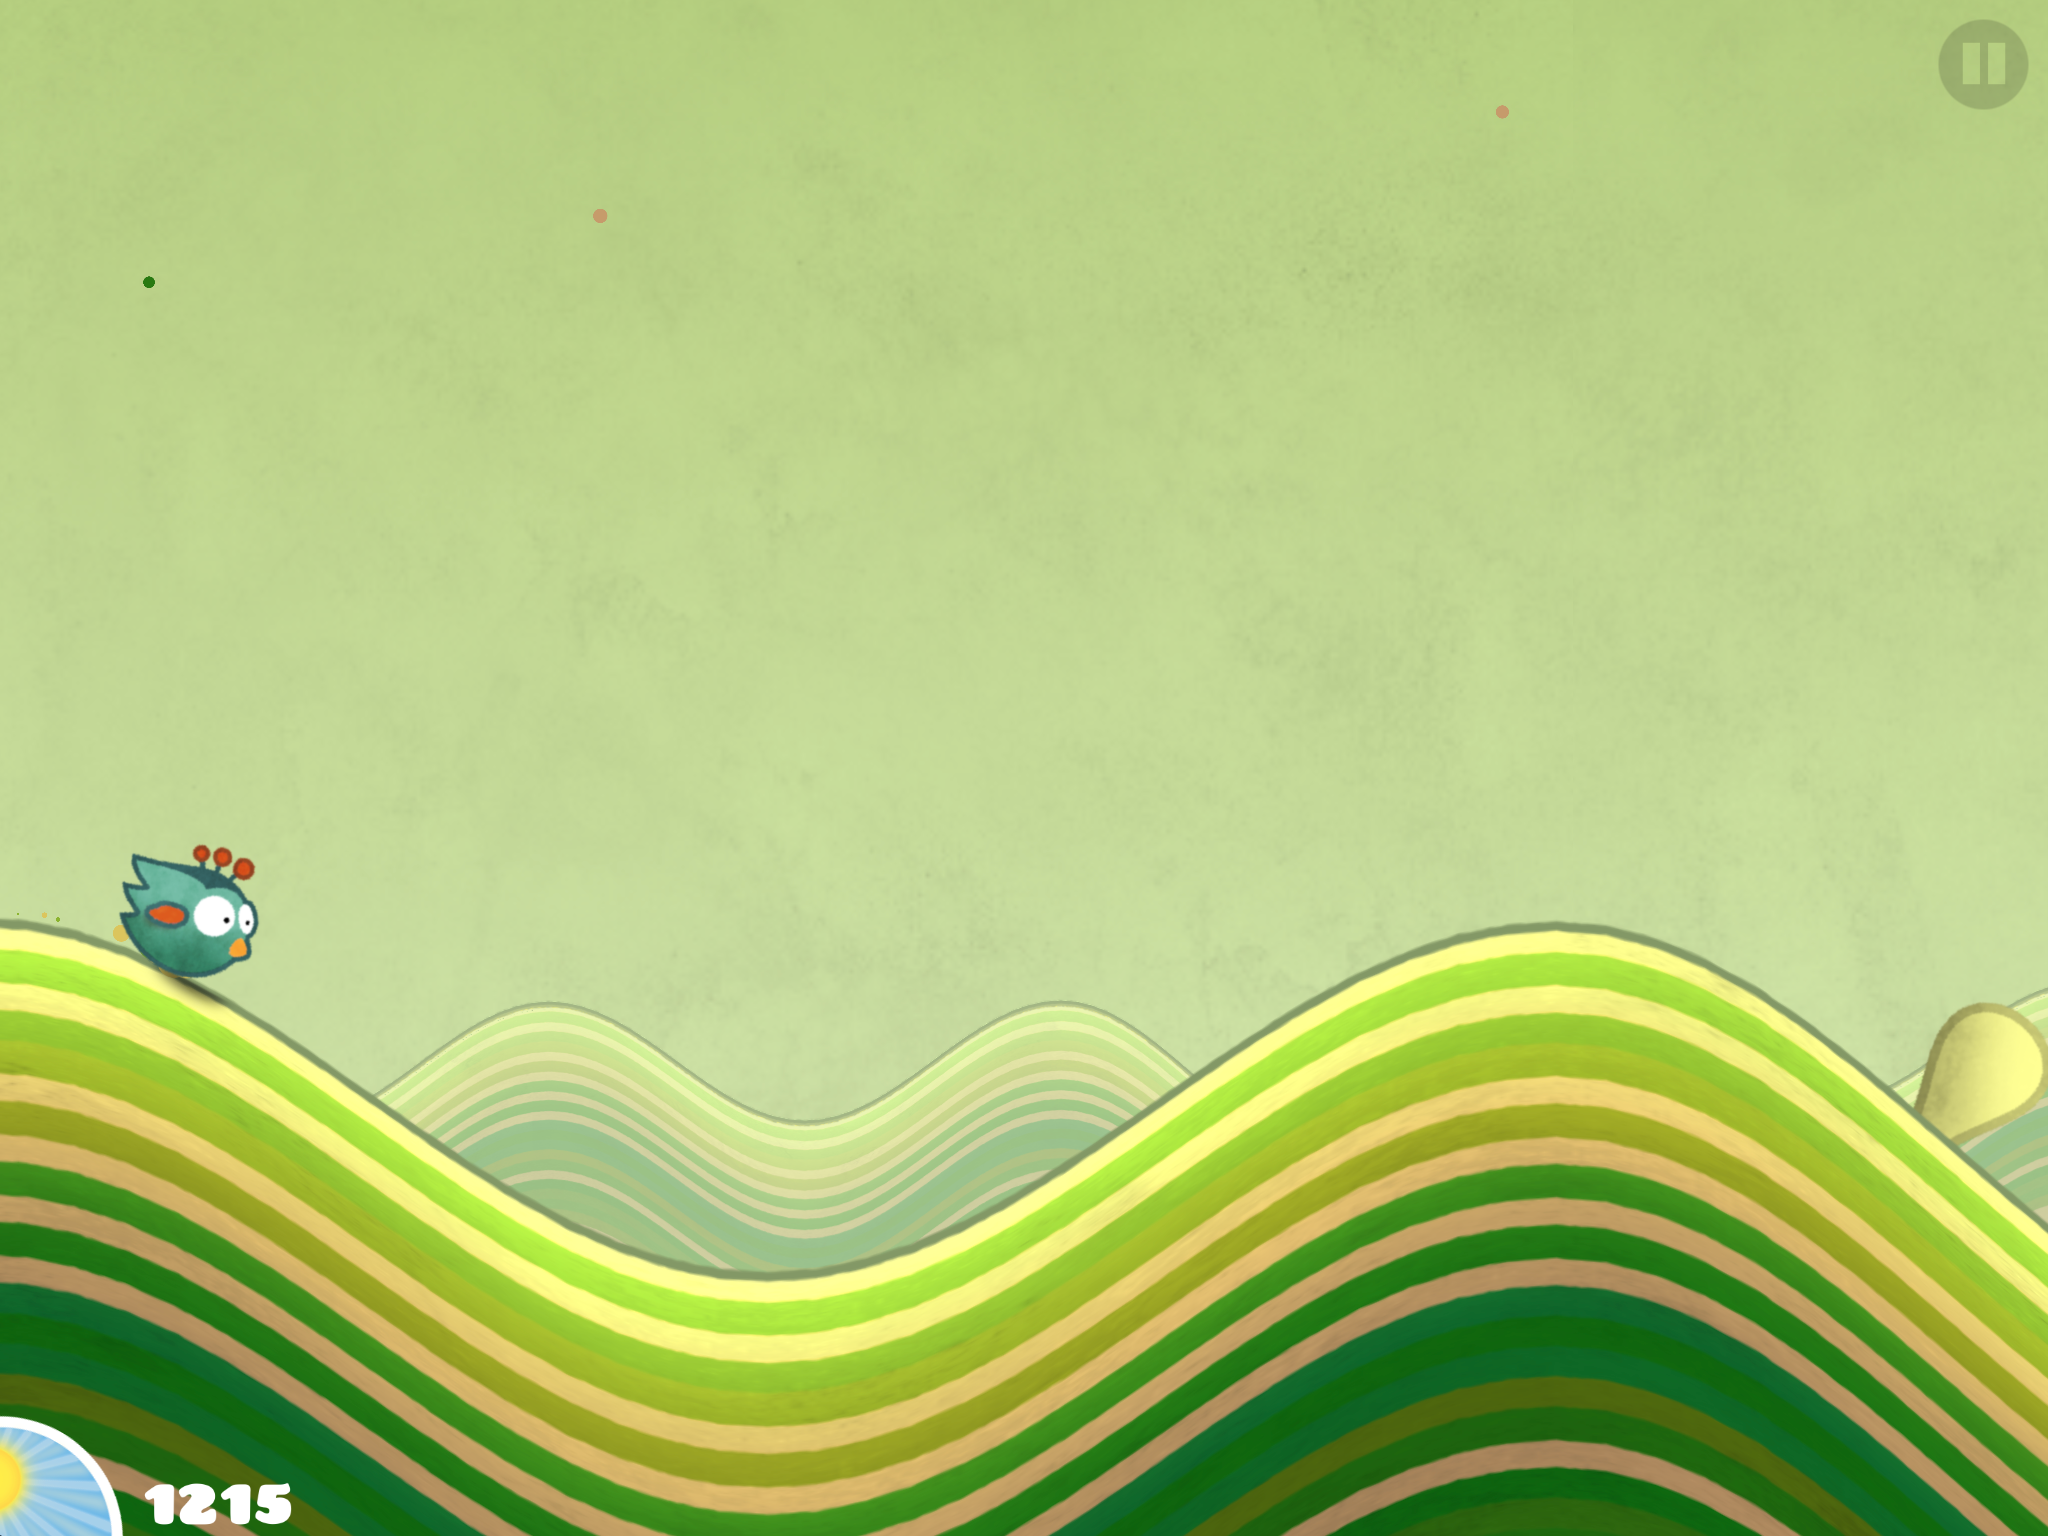
\includegraphics[width=\textwidth,height=0.62\textheight,keepaspectratio]{figures/fig01.png}
\end{center}

我从事理论研究与算法开发工作也恰恰像是翻越一座座连绵起伏的山脉。每一次登顶后，都能收获不尽的欣喜（ecstasy）与鼓舞（encouragement）。然而，这种如释重负（relieving）的感觉往往是转瞬即逝（ephemeral）的，因为眼前会立刻浮现出（loom up）更加高大、巍峨的山峰以待我去征服。此时，我不得不让兴奋的头脑冷静下来，重置在刚刚达成目标、收获成功后的“轻浮”心态，重新聚集力量（strength）、耐心（patience）、专注（focus）、细心（meticulosity），仿佛一切又从零开始一样。

“不忘初心”的口号容易让人获得一种虚无的信心与空洞的自豪。但当它对应到具体的实践与真实的生命体验时，就会以上述清零、重置、重启的感觉呈现，这已近乎无助的努力与绝望的抗战。然而，只有身处于这种体验与状态时，我才会觉得一切都是合理的、正确的、正常的（Alles in Ordnung）。因为这才是开发者的真实状态，也是事物从无到有、不断提升的一般规律，更是有志于学者求仁得仁的命运。

\begin{classic}
《论语·述而篇第七 7.15》冉有曰：「夫子为卫君乎？」子贡曰：「诺，吾将问之。」入曰：「伯夷、叔齐何人也？」曰：「古之贤人也。」曰：「怨乎？」曰：「求仁而得仁，又何怨？」出曰：「夫子不为也。」
\end{classic}

\entrydate{2023.06.15}

\chapter{从心所欲不逾矩}

我在学习与研究的过程中越来越频繁地发现，无论是记笔记、数学推导、代码编写，还是撰写报告与文章，都不再是一蹴而就的，而演变为一个多次迭代、逐步完善的过程。与此同时，在这个过程背后必有一个大致的目标——其实，该目标倒也不一定非常清晰明确，因为我往往都是在黑暗中前行，在未知或者一知半解中摸索的——和一些基本思想、设计原则，以及一贯的做事风格与工作态度等非智力的、无法量化的要素作为冥冥之中的引导。这种模式与我在学生时代的压力与忙碌中为了完成作业、应对考试、准备毕业论文的学习与研究方式是完全不同的。它要求我必须扫除内心所有的浮躁与急迫，以一种不得不依照通过长期持续的科学探索直至有所心得、有所发现需遵循的一般规律来做事。其间绝不能有逻辑上的跳跃与模糊不清，亦容不得弯道超车与自吹浮夸，只能以无比坚实的耐心与细心来推进工作。

一开始，我按这样的方式做事可以说是出于无耐，因为只要有丝毫的马虎大意，出错就总是必然的——这一点我从每次修改程序后第一次编译很容易出错这一现象就可以看出。后来，慢慢地变成了一种“逆来顺受”，且直到今天依然如此。最终，我想应该努力达到从心所欲不逾矩的境界。

\begin{classic}
《论语·为政篇第二 2.4》子曰：「吾十有五而志于学，三十而立，四十而不惑，五十而知天命，六十而耳顺，七十而从心所欲，不逾矩。」
\end{classic}

\entrydate{2024.10.01}

\chapter{命运的最好安排}

算法开发与测试是一项需要高度专注、细致、耐心的工作。因此，动手干活前就不能急躁、毛糙，要将目标和步骤都想清楚后再逐个落实。当然，由于需要处理与消化的信息量较大，且随着个人年龄增长可能出现的记忆力衰退问题，大脑就会记不住那么多信息。此时，可利用白板、思维导图、KNote、Xournal++ 等软硬件工具，将步骤与要点列清楚，将想法用最自由与直接的方式予以表达和记录。不要因为怕麻烦或者不愿切换工作环境与条件而不去启用这些工具。它们就相当于我们无限大的稿纸、记忆力的延伸、工作内存的拓展、想象力的激励。没有这些工具的辅助，仅依赖自己的心算、空想和机械式地推演，是无法将信息内化为理解，也解决不了复杂与深奥的问题的。

上述专注、细致、耐心的工作态度恰与我自己中小学逐渐培养起来的学习态度是一致的。回想起来，在以前的学生时代，我将课本、笔记、习题集、考卷反复揣摩、提炼、重构了无数遍。在每一次的考场上，我虽然在考试结束前很早就已完成了答卷和检查，但仍旧能够 \textbf{不厌其烦} 地在稿纸上多次演算、验证，以确保解题步骤、措词行文、最终答案万无一失、完美无缺。这个过程其实是非常枯燥与乏味的，与我如今在算法开发过程中百思不得其解地调试程序极为类似。而以往通过不断磨炼形成的习惯与风格，正好恰如其分地用在了当前数值算法开发这种精细、精密的工作中，使我获益匪浅。

由之前的因，逐渐形成今日的果。能够让多年以前的素质、态度、模式在当前和未来持续发挥关键性的作用，这便是命运的最好安排！想来，这也是孔子所说的“吾道一以贯之”在科学研究上的具体体现。

\begin{classic}
《论语·里仁篇第四 4.15》子曰：「参乎！吾道一以贯之。」曾子曰：「唯。」子出。门人问曰：「何谓也？」曾子曰：「夫子之道，忠恕而已矣。」

《论语·尧曰篇第二十 20.3》子曰：「不知命，无以为君子也。不知礼，无以立也。不知言，无以知人也。」
\end{classic}

\entrydate{2024.01.30}

\chapter{无友不如己者}

虽然我并不是顶级聪明的人，但是在实践中发现，通过长时间地思考和玩味一个问题，确实能够使自己的认知获得质的提升。这个提升的达成是随机出现的。你可以把这个现象归因为灵感和运气。虽然看似飘忽不定、不可捉摸，但其产生是有必然性的。因此，在长期保持专注的前提下，对于顿悟与灵光一现要抱以十足的信心。这是对于勤能补拙这个道理在实践上的验证，而不仅仅是在理性与情感上的形式认可。所以说，王阳明“知行合一”的说法是绝对正确的，只有通过笃行才能够获得对人生、做事等各方面道理的真正理解。

耐心、细致、扎实地工作，不要着急。既要自由涂鸦、大胆改动、发散思考，又要耐心、谨慎地推理，不断调用和累积细致入微的知识点。要通过反复的训练、反省、改进，将这两种工作模式很好地融合起来，做到从心所欲不逾矩。虽然开发区域分解算法涉及的细节和步骤非常多，而且他们在脑海里的浮现也是有一定的随机性，越是这种看似的紊乱，越要耐下性子，一点一点地做，一点一点地想和记录，最终一定能够从纷繁芜杂中逐步走出来。

面对这种复杂的开发工作，也越来越深刻地体会到工具的重要性。譬如机械加工，高精度的零件只有借助精密的机器、精湛的技艺、合理的加工流程才能做出来。同样的，无论是理论推导、软件设计、算法开发，还是记笔记与信息管理，工具的功能是否足够强大，你对它是否投入了足够的时间以便操作熟练并且持续扩展其功能、提高效率，在很大程度上决定了你能够做成事情的复杂度、精密度和质量。所以，任何时候都不要投机取巧，都不要为了图快而采用退而求其次的方案。所以，将正则表达式、软件项目构建与调试工具、二进制文件的操作命令等基本工具用对、用熟、用好，才能完整地实现自己的设计思想。否则，就只能是处处妥协，处处打折扣，浮沙筑台，最终根本构建不起大的项目。

当下碎片化信息多以短视频形式传播。长篇表达如会议演讲、系统化信息讲授如大学课程也多以视频形式发布。然而，话虽说得好，道理讲得通透，经过了前期设计与后期制作，表达形式也变得生动光鲜，但大多容易陷入巧言令色、论笃行浅的境地。对此，我们要予以明辩：究竟主讲者是真君子、真学者，还是仅仅表现得人模人样，只有言语技巧或者文字功夫。一个评判的标准是，不要看这个人说了什么、领导或组织了什么，而要看这个人亲力亲为做了什么，实践过程是否贯彻了其所讲的思想与原则，收获的成果是否也体现了同样的品质精神。

\begin{classic}
《论语·先进篇第十一 11.21》 子曰：「论笃是与，君子者乎？色庄者乎？」
\end{classic}

因此，我们根本不必知道那些不如自己或跟自己差不多水平的人所做的工作以及采用的态度、方式。要和这个世界上最优秀的、亲力亲为的人对比、参照，以他们为榜样，如 Linus Torvalds，Richard Stallman。想要有真正的创新，想要做出能够打动人心的工作，首先就不能对现实妥协，要敏锐且不留情面地发现其中的问题，不断改进。若只是被动地适应周遭的环境，成为与中低水平同类内卷过程中的赢家，最终看似收获颇丰，但那只不过是病态的毒瘤，越多反而越糟。千万不要以为大的、多的就是好的。真正的优雅和顶级的品质与数量和规模无关。

\entrydate{2024.08.23}

\chapter{如何面对“无底洞任务”}

我们在生活中总会遇到一些工作量大到几乎是无穷或者难以估计的任务，如数学学习与研究这类既重要又紧急的工作。它们堪称消耗个人时间和精力的无底洞。而如何将其与生活中的其他事务平衡与协调起来，就成为一个颇为困扰的问题。毕竟，个人学识的长进与修养的提升是无法仅凭藉在单一或极少数几个领域中的专注就能够达成的。这是因为不同领域在思想方法和“悟道”的层次上都是相通的。例如，通过音乐、体育的训练总结出的有效方法、宝贵经验，甚至仅仅是一些流动的心理感受，就可以触类旁通、移花接木般地从中收获对纯粹理性工作的启发。此外，生活中亦还有其他非常重要的事情需要精心打理，如家庭、亲情、友情的经营与维护。然而，“无底洞任务”的存在势必会在时间、精力、心理上对其他任务产生强大的挤压作用，令人极难作出决策与取舍。

对此，我觉得如果能够把握以下三个原则，将会有助于上述困境的解决。

\begin{itemize}
\item 要构建并固化属于个人的学识发展框架。这相当于站在完整人生的战略高度，在整体架构和门类上对个人的学习、研究、工作、爱好的范畴予以界定。而“无底洞任务”无疑就是这个框架的基石或核心。这也就是儒家思想中的“止于至善”、“君子务本，本立而道生”。立于这个坚如磐石的基础上，一个人才会对“无底洞任务”的规划与执行产生信仰般的持久动力。否则，无论外在环境或者他人的观点意见有任何惊涛骇浪或细小波澜般的变动，你的心态和行动都会受到影响和干扰，此即“小人之德草，草上之风必偃”。
\item “罗马不是一天建成的”。即便是焚膏继晷、不饮不食，也不可能在短时间内搞定“无底洞任务”。所以，还是放弃这种不切实际的念想吧！相反，要将其当作长期的追求。不过，需要留意的是，万万不可把长期的追求抽象地扩展为“毕生”的追求。那样一来，就没有了紧迫感，无法形成自我压力。稍有不慎，就变成了踩着西瓜皮行走，得过且过了。因此，需要制定带有截止日期的中长期计划。关于计划的作用可以参考罗辑思维第236期《计划的用处》。其中提到了计划并不是为了死板和教条地照章办事，而是给自己创造出一个可以基于理性思考的判断、评估和决策的机会。同时，计划亦是在团队中达成共识、形成凝聚力的必要因素。至于现实中会出现什么样的变化，则可以根据具体情况予以更改。
\item 将“无底洞任务”拆解为可以执行的步骤。只有做到对于细节任务的明晰与把控，才不至于在宏观问题上产生迷茫甚至动摇。若你觉得“无底洞任务”令人畏惧，深不可测，那就证明你对于如何开展和实施它们思考得不够多、不够细，以至于拿不出一个成文的任务清单。而一个经过理性思考后得出的任务清单即便不甚合理，也总比什么都没有强。更何况，任务分解的合理性也并不是一个可以先验地予以回答的问题。相反地，只有通过具体的执行逐渐获取更多的信息，并时时反思、修正，才可以逐渐地逼近真值。可以看出，“敏捷开发”的思想方法也在此得到了应用。在任务分解的过程中需要秉持的心态是：“磨刀不误砍柴工”，宁可慢，不宜快。虽然从最初的分析、思考再到最终的成形需要花费很多时间，但是这样的投入能够保障人生航向的正确或者是自以为正确，从而获得强大的自信与自我说服力，因而是极其值得的。
\end{itemize}

总之，如果你的生活中存在“无底洞任务”，虽然表面上看似可怕，但也未尝不是一件好事：因为这至少证明了在你的生命中还存在值得长期坚持的元素，它们的价值和意义远远超出了每天朝九晚五的工作和柴米油盐的生活。然而，为了把“无底洞任务”和自己的生活协调好，就需要信仰般地确立属于自己的学识架构，在宏观上为其制定出带有截止日期的中长期计划，在微观上拆解出可以照章办事的任务列表。同时需要注意的是，计划的存在绝不意味着教条与死板，而是意味着理性思考和对不断变化环境的自适应。

\begin{classic}
《论语·学而篇第一 1.2》 有子曰：「其为人也孝弟，而好犯上者，鲜矣；不好犯上，而好作乱者，未之有也。君子务本，本立而道生。孝弟也者，其为仁之本与！」

《论语·颜渊篇第十二 12.19》 季康子问政于孔子曰：「如杀无道，以就有道，何如？」孔子对曰：「子为政，焉用杀？子欲善，而民善矣！君子之德风，小人之德草，草上之风必偃。」

《论语·子路篇第十三 13.17》 子夏为莒父宰问政。子曰：「无欲速，无见小利。欲速则不达，见小利则大事不成。」
\end{classic}

\entrydate{2017.11.26}

\chapter{数学与长笛}

数学理论的大厦乍一看上去令人瞠目结舌：其规模的宏大伟岸，外延的似无边际，内涵的深不可测，抽象分类的层出不穷，逻辑联结的精密繁杂，以及千变万化的诸多变换，令人深感自身渺小，不由心生敬畏甚至恐惧。然而，若将其拆解为一个个细小但彼此相连的定义、定理，我们就还是可以如同蚂蚁啃骨头一般，把它们逐渐理解、消化乃至最终掌握的。

与数学类似，长笛演奏同样是一门博大精深的学问，而且还包含了很多难以言表、只能先经老师点拨再靠自己体悟的技能、艺术。尽管如此，也还是可以在练习的过程中将其拆解为不同的方面，如基本功、练习曲、表演曲、乐理。其中，基本功又可以分解为长音、颤音、双吐音、强弱变换、基于音阶的快速指法等。而练习曲和表演曲则可划分为很小的乐句乃至每一个小节，然后精雕细琢、精益求精地去练习。这包括对于指法的感受和熟悉，呼吸与情绪的把控，强弱、快慢和节奏的处理，音色与表现力的微调等等。乐理知识则是一门独立的学问，需要以研究的心态来吸收、揣摩。

由以上可以看出，数学学习和长笛练习是相通的。她们无一不是要经过仔细考虑、反复斟酌、不断强化练习和“如临深渊”般的精准控制。毕竟，要想臻于完美，就需要在修炼和磨练的过程中克服畏难情绪，拥有无与伦比的耐心，付出大量的苦心和苦功。

\begin{classic}
《论语 子罕 9.15》子曰：“吾自卫反鲁，然后乐正，雅颂各得其所。”

《诗经 小雅 小旻》战战兢兢，如临深渊，如履薄冰。

《论语·泰伯篇第八 8.3》 曾子有疾，召门弟子曰：「启予足！启予手！诗云：『战战兢兢，如临深渊，如履薄冰。』而今而后，吾知免夫！小子！」

《论语·学而篇第一 1.15》 子贡曰：「贫而无谄，富而无骄，何如？」子曰：「可也，未若贫而乐，富而好礼者也。」子贡曰：「诗云：『如切如磋，如琢如磨』，其斯之谓与？」子曰：「赐也，始可与言诗已矣，告诸往而知来者。」

《论语·八佾篇第三 3.23》 子语鲁大师乐，曰：「乐其可知也：始作，翕如也；从之，纯如也，皦如也，绎如也，以成。」
\end{classic}

\entrydate{2017.10.26}

\chapter{学习与研究自由}

自学数学最好能配有一本与个人拥有的理论基础和知识体系、对学科背景和发展历史的了解程度、习惯的逻辑推演和表述方式相契合，且推导过程细致入微、鲜有逻辑跳跃，同时又能上升到方法论层次而授人以渔的优秀教科书或专著。单就内容组织与数学推导的细致程度来说，当以德国人的著作更胜一筹（Teutonic thoroughness）。正所谓凡事怕认真二字，而“细致”便是“认真”的一个重要而具体的体现。

若想在我们的研究历程中与这类著作邂逅并产生交集与共鸣，首先需要自身的刻苦努力。毕竟，只有通过广泛阅读与一定深度的学习，才能对涉及同一领域、同一研究问题的不同著作有所切身感受和对比，由此才能作出选择。网上的书评与书单只代表了他人的感受与意见，因而仅能作为我们文献调研的参考与起点，而绝不能替代我们自身的实践、体验与评判。其次，能够遇到适合自己的书籍也需要某种难以捉摸和把控的缘分。不过在当今信息资源丰富、搜索工具强大便利的条件下，能够找到属于自己并引领我们进入更宏伟理论殿堂的书也变得相对容易些了。

上述调研、阅读、评判的过程，恰是促进我们实现 \textbf{学习与研究自由} 的重要一步。而这个自由远胜过财富自由。毕竟，变富虽能让一个人用财富杠杆轻松撬动“现实”成果，但也容易使其计较过多、乐不思蜀，从而成为在“求真”层面上自我提升的障碍，并终究难以重返宁静、深思冥想、付出苦功、下学上达。

\begin{classic}
《论语·宪问篇第十四 14.35》 子曰：「莫我知也夫！」子贡曰：「何为其莫知子也？」子曰：「不怨天，不尤人，下学而上达。知我者，其天乎！」

《论语·学而篇第一 1.15》 子贡曰：「贫而无谄，富而无骄，何如？」子曰：「可也，未若贫而乐，富而好礼者也。」子贡曰：「诗云：『如切如磋，如琢如磨』，其斯之谓与？」子曰：「赐也，始可与言诗已矣，告诸往而知来者。」
\end{classic}

\entrydate{2022.07.03}

\chapter{三人行，必有我师焉}

现在回想起来，自己曾在大学从本科到博士后度过了整整十一年的荏苒时光，而屈指算来人生也就不过八到十个十年而已。原以为自己的人设就是在学校终老一生、与学术为伴的，但最后也从中跳出来到了外企工作，至今竟也整整七年了。虽说学校是学生们得以专注学习、潜心研究的象牙塔，是慎思博学的风水宝地，但一个人到了工作中、社会上，只要凡事处处留心，待人虚怀若谷，也仍有不少甚至是学校都难以或无法提供的学问与心法。本文便将我工作数年期间从学长、同事那里学到的思想方法与相关的个人心得体会整理罗列出来，旨在通过回顾与重温来加深印象，从而既有助于自修，也提醒自己不忘感恩，此外若还能对更多的人有所启发与裨益，则更是值得欣慰了。

\begin{itemize}
\item 搜索与阅读专著和文献时，需要带着明确目标去查阅真正对解决问题有用的材料。要有细节但又不能拘泥于细节。要能够分清不同任务的轻重缓急，明确什么是自己最擅长的，什么又是自己需要去发展的。这应该就是做科研的艺术！由此，才可以确定应该在哪些事上做得更底层一些，而在哪些事情上又需要大胆地站在前人的肩膀上，利用他们已有的成果。
\item 眼高手低是做技术者的大忌，尤其是自以为智商过人的时候。即便是对于已经掌握较好的技术，也不能因骄傲和自满而停滞不前，应该持续学习、不断提升，达到行云流水的境界。
\item 无论是纯粹理论的推导还是工程技术方案的实现，都像是俄罗斯套娃一样层层相套、相扣。只有不厌其烦，逐层地打开这些黑盒子，尽可能展开更多的细节，才能够暴露更多潜在的问题。也只有如此，才能够获得大量数据用以澄清问题，并将其逐一解决，从而最终保证整个技术实现的完全精确与可靠。
\item 止于至善的精神不仅仅适用于长期的、终极的人生，也完全适用于项目工作的开展。至善，就像是油画中的所有细节那样，是不知经过多少次细枝末节的修改、增删而一层一层地积累起来的。想要止于至善，就必须培养起足够的乃至惊人的耐心与毅力。不怕慢，不怕细，不怕反复，更不怕屡次的失败与推倒重来！
\item 面对不直接参予技术实施的项目负责人以及对技术只知皮毛概念的高层管理者，要想阐释什么是正确的、证明什么才是真理的最好方法不是用数学和物理理论，而是实验数据和技术演示。因为到了职场中、社会上，已经鲜有人有能力和耐心去跟你一起做逻辑推演了。
\item 要想让项目提议获得管理层的认可，并在其实际支持下从幼苗成长为大树，需要编制与展示完整的用户故事，而不是灵光一现的理论方法、前沿技术，即便该理论与技术是项目的核心与精髓。毕竟，对于管理层与最终用户来说，直接创造价值的是产品不是技术。从另一方面讲，被人认可的只是产品的实用价值而无人关心和欣赏背后的设计，这也是科技工作者的悲哀。正所谓，“欲将心事付瑶琴，知音少，弦断有谁听？”。
\item 对于技术可行性一定要有明确的表态，尤其是能否做成的表态。否则，会让别人做出错误的决策，以至于本来还有其他挽救的方案但却没有采用。
\item 进入职场的时间长了，人就容易疲，容易自满与浮躁。此时，要将自我清零，像小学生面对老师一样，怀着一颗无比耐心与踏实的心。
\item {\kaishu 《大学》中说到的“正心诚意”，不仅指对待自己的本职工作，在给同事提供力所能及的协助时也应同样如此。这便是“尽己”与“不辱使命”。}
\end{itemize}

\begin{classic}
《论语·述而篇第七7.22》 子曰：「三人行，必有我师焉：择其善者而从之，其不善者而改之。」
\end{classic}

\entrydate{2018.10.27}

\chapter{文献阅读方法改进}

在学术文章与专著的阅读方面，我发现自己稍不留神便常常走入如下两个极端：

\begin{itemize}
\item 过尤不及：过于认真地阅读以至进度极其缓慢。虽然也吸收了相当多的细节内容，但却对原本的学习目标贡献寥寥。这种情况便是事倍功半。（《论语·先进篇第十一11.16》 子贡问：「师与商也孰贤？」子曰：「师也过，商也不及。」曰：「然则师愈与？」子曰：「过犹不及。」）
\item 走马观花：一味追求效率和进度，以跳跃和不求甚解的模式浏览原文。结果看了一圈下来，不晓得主旨，抓不住要领，白白浪费了时间和精力。这时，所谓的效率其实已经“堕落”成浮躁，实质性的进度则为零。（《论语·子路篇第十三13.17》 子夏为莒父宰问政。子曰：「无欲速，无见小利。欲速则不达，见小利则大事不成。」）
\end{itemize}

由此可以看出，在认真细致与高效粗略之间，我还拿捏不好分寸。需要进一步通过提高阅读量、记录和整理出的笔记量（关于笔记量，在《The Man Who Knew Infinity》一书中讲到拉马努金（Ramanujan）每月都要写两千多页（He'd need four reams of it a month.）的数学推导和演算草稿。与在如此专注和勤奋的状态下产出的工作量相比，我还有相当大的差距。），以及复习的频率，以期得到改进。具体的整改措施罗列如下：

\begin{itemize}
\item 在开始阅读前，明确自己的阅读目标（target）、期望的收获（deliverable）和预计投入的阅读时间（resource）。在训练初期，由于对阅读技巧的把控尚未做到游刃有余，需将这三方面内容逐条清晰且尽可能量化地列在清单中。然后，便可以该清单作为阅读过程中的即时提醒和阅读完成后的考核标准。注：这里所谓的即时提醒，起到的是“君子无终食之间违仁”的效果。（《论语·里仁篇第四 \quad 4.5》子曰：「富与贵，是人之所欲也，不以其道得之，不处也。贫与贱，是人之恶也，不以其道得之，不去也。君子去仁，恶乎成名。君子无终食之间违仁，造次必于是，颠沛必于是。」）
\item 在需要认真细读的地方，应以期望的收获作为指引，把每一个环节都想得如水晶般透彻，并工整地做好笔记。笔记的整洁与否，以及是否具有形式上的结构化、内容上的条理性和最终体系的完整性，能够反映出一个人的心态是平静还是躁动，思路是清晰还是紊乱，思想是深刻还是浮浅。因此，不可不引起高度重视。
\item 在需要高效略读的地方，要围绕自己的阅读目标，紧紧抓住文章或书籍的主旨思想、重要方法、技术环节、主要结论等几个关键要素，从而展开快速的阅读活动。不应一味徒快，以至于花费了时间与精力，但脑海仍旧空空如也。
\end{itemize}

\begin{classic}
《论语·先进篇第十一 11.16》 子贡问：「师与商也孰贤？」子曰：「师也过，商也不及。」曰：「然则师愈与？」子曰：「过犹不及。」

《论语·子路篇第十三 13.17》 子夏为莒父宰问政。子曰：「无欲速，无见小利。欲速则不达，见小利则大事不成。」

《论语·里仁篇第四 4.5》 子曰：「富与贵，是人之所欲也，不以其道得之，不处也。贫与贱，是人之恶也，不以其道得之，不去也。君子去仁，恶乎成名。君子无终食之间违仁，造次必于是，颠沛必于是。」
\end{classic}

\entrydate{2018.10.09}

\chapter{避免对工具的痴迷}

工具作为拓展人类智力与能力的利器，其自身所具备的功能、性能、可扩展性的重要意义毋庸置疑。一个人也应当持续不断地通过刻意练习来提升使用工具的能力，达到熟能生巧、能够自然流畅地表达设计思想与技术理念的效果。但与此同时，亦不要对某种技术或者软件工具怀有太多的感情与痴迷，更不要卷入诸如网上Vimer与Emacser之间的论战与纷争。这主要是出于下面的考虑。

一个工具的流行程度会随着时代的变迁与技术的演进而不断变化，甚至完全被淘汰。举例来说，曾经红极一时的Perl语言如今逐渐淡出人们的视野，而昔日因性能太慢而被大家鄙视吐槽的Python反倒成了当下大红大紫的名星。因此，优秀的科技工作者应该关注隐身于工具与技术背后那些真正稳定甚至是永恒的要素：设计思想（包括数据与算法的抽象、软件的组织架构等）以及需要解决的具体问题（“解决问题”、“改善生活”是人类得以延续和发展的持续动力）。然后，在此基础上更进一步，通过数学【理论】与泛型编程【实践】的高度抽象来解决一大类问题而非单个案例。相反地，不能仅仅因为已经在一个技术上投入了大量学习与实践的时间并拥有了相当多经验与技能的积累，便始终持有一份情怀与坚持不放。这样一来，身上背负的“历史”包袱只会越来越重，最终则被时代无情地抛弃。总之，大多数的技术需要深厚的积累方能形成强大的生产力与推动力，但却不能固守。开发者仅将它们当作称手的工具解决当下的问题，不需要的时候扔掉即可，与时俱进。

换个角度来看，最终用户关心的则是由工具创造出的产品而绝非工具本身。除了开发者自己对于工具有着一份执念与情怀外，用户是丝毫不会关心工具本身有多么强大和先进的。开发者能够与用户建立起的唯一接口就是产品能够达到的性能、实现的效益和形成的体验。因此，理性的开发者应当更多地关注用户的需求与体验，通过整合现有的知识与工具勾画出完整的“用户故事”，精益求精地实现与之相应的解决方案。这也是《论语》所说的“吾日三省吾身，为人谋而不忠乎？”。

\begin{classic}
《论语·学而篇第一 1.4》 曾子曰：「吾日三省吾身，为人谋而不忠乎？与朋友交而不信乎？传不习乎？」
\end{classic}

\entrydate{2020.06.13}

\chapter{“学之不讲”是吾忧也}

\begin{classic}
《论语·子罕篇第九 9.29》子曰：「知者不惑，仁者不忧，勇者不惧。」

《论语·述而篇第七 7.3》子曰：「德之不修，学之不讲，闻义不能徒，不善不能改，是吾忧也。」
\end{classic}

“学之不讲，是吾忧也”，这句话恰如其分地描述了我现在的心情：面对积累的越来越多的知识，我对它们并非全都有过具体、反复的操练，所以根基并不扎实，前学后忘便很难避免。在做事、实践的过程中，我总会感到“书到用时方恨少”。但与此同时，又不能陷入复习、练习的无限循环中，而始终不能从中跳出来做事、实践。单独来看学习、复习、练习、实践，每一项似乎都还可以应对（当然，否能够做得好就另当别论了）。但将这四者放在一起，且考虑随时间积累的倍增因素，就会发现时间根本不够用，人生的紧迫感也就由此而生。

这也就是为什么虽然孔子曾说过“仁者不忧”，但具体到做学问乃至修德、行善的时候，面对人生“不舍昼夜”的紧迫感，忧虑就不可避免了。然而，只是忧虑是不行的，还要将其化解，将压力转变为动力，再以放松的身心投入到做学问中，这样才能获得最好的效果。在这一点上，孔子的做法则是直接或者间接地（通过文学作品）走入与感悟大自然，即 living in communion with nature。例如，

\begin{classic}
《论语·先进篇第十一 11.26》「莫春者，春服既成；冠者五六人，童子六七人，浴乎沂，风乎舞雩，咏而归。」夫子喟然叹曰：「吾与点也！」

《论语·雍也篇第六 6.23》子曰：「知者乐水，仁者乐山。知者动，仁者静。知者乐，仁者寿。」

《论语·阳货篇第十七 17.9》子曰：「小子！何莫学夫诗？诗，可以兴，可以观，可以群，可以怨。迩之事父，远之事君，多识于鸟兽草木之名。」

《论语·子罕篇第九 9.28》子曰：「岁寒，然后知松柏之后雕也。」

《论语·子罕篇第九 9.17》子在川上曰：「逝者如斯夫！不舍昼夜。」

《论语·乡党篇第十 10.27》色斯举矣，翔而后集。曰：「山梁雌雉，时哉时哉！」子路共之，三嗅而作。
\end{classic}

同时，聆听音乐也是对心灵最好的净化与抚慰。

\begin{classic}
《论语·八佾篇第三 3.23》子语鲁大师乐，曰：「乐其可知也：始作，翕如也；从之，纯如也，皦如也，绎如也，以成。」

《论语·述而篇第七 7.14》子在齐闻韶，三月不知肉味，曰：「不图为乐之至于斯也。」

《论语·泰伯篇第八 8.8》子曰：「兴于诗，立于礼，成于乐。」

《论语·子罕篇第九 9.15》子曰：「吾自卫反鲁，然后乐正，雅颂，各得其所。」
\end{classic}

两千多年过去了，以上这些语录依旧能给我们带来心智的启发与实践的指导，想来真的是很神奇。相较于科技发展的日新月异，人性真的是蛮稳定的。

\entrydate{2024.05.02}

% 职场.tex
% Auto-generated from 感悟论语.odt by tools/odt_to_tex.py

\setpartplant{artwork/plum.png}
  {梅}
  {磨而不磷，涅而不缁。}
  {《论语·阳货》}
  {职场}
\part{职场}

\chapter{不存在“35岁陷阱”}

\begin{classic}
《论语·为政篇第二 2.12》子曰：「君子不器。」
\end{classic}

网上经常看到一些互联网企业清退那些大于等于35岁的员工，于是也便有了所谓“35岁陷阱”的说法。然而，一个人从知识体系的逐渐完善与纯熟，到设计思想的持续精进，再到技艺经验的不断锤炼与提升都是一辈子的事情，而且是没有上限的。企业硬生生地以35岁作为划分雇佣与清退的界限，只能说明不论企业表面上声称的如何，在事实上他们一直无情地将员工视为器物和工具；而且因企业本身的功利、短视、平庸，对这些“器物和工具”的利用也只是局限在较低的层次上，因而有意识地完全忽略和埋没了员工作为一个真正的人本来所具有的无限潜力。

对此，打工者不能因为企业的无理清退或是耳闻目睹到了相关的消息便给自己灌输那种“人到了一定年龄，学习、研究、编程就会干不动，记忆力与工作效率也比不过年轻人”的错误的潜意识。正确的态度是始终做自己的主人，持续提升、超越自我、止于至善。

在具体的方法上，则需要观察与评估我们是否已做到了问心无愧的努力。同时，也要反思我们采取的学习方法是否正确得当，否则便会陷入“学而不思则罔，思而不学则殆”的困境。再者，审视一下我们是否具备了良好的态度与性格。这包括无比的耐心与细心，无所畏惧、迎难而上的勇气，不怕麻烦地“敏于事、慎于言”。对此，《三体》一书也提到，真正的基础研究反倒需要不那么聪明（滑头）的人来搞——因为只有这样的人才能做到在科学面前踏实、严谨、谦虚、虔诚，从而保证了逻辑的缜密，也没有任何先入为主的自以为是。

拥有了以上正确的思想与态度，我们还需要注意身心、生理的健康。在学习与工作的过程中，我们需要保持高效但却放松的身体与精神状态，从而在最大程度上延长我们的学术与技术生命。例如，可以适当地将我们书写、打字的速度放慢下来，从而避免因过度用力而产生的肌肉紧张与劳损，也能使我们更好地感受、体会和记住在专注状态中的细微体验。这样会有助于培养我们的肌肉记忆，令技艺更为精湛、纯熟。

总之，企业没有拿员工当作真正的人来对待，员工也便不值得为企业卖命付出。打工者不要被企业设定的种种规则、制度、指标蒙蔽双眼，甚至是陷入怀疑、焦虑、恐慌。相反地，打工者要启发自己的心智，为自身的提升与精进不断努力，最终做自己生命与事业的主人。

\entrydate{2021.01.07}

\chapter{君子无终食之间违仁}

时至今时，仍然时常想起高中化学老师对我的教诲：“学习知识就要像牛儿看到满山的青草一样如饥似渴”。由此，亦回忆起我在高一时于一个周六严热的下午上化学奥赛课，一下子塞进了那么多的知识（第IV与V族元素）。可见，在将自己完全清空、严格按照训练规定去做的时候，能够产生多么巨大的动力。而且，总是可以把内在、外在的各种压力转变为动力。现在距离高中时代已近二十年了，我仍应保持那份初心与动力。原先是个人、家长、学校、老师、社会全方面对我产生的约束作用。现在能够起到监督作用的只能是靠自己。然而，君子贵在慎独、慎微，应从点滴和当下做起。

走上工作岗位后的研究与中学的学习不同的是：以前学生时代所学的都是已有的、纯粹经典的内容。那时的我不光记忆力好，还经过了无数次的反复与巩固，因而可以做到熟稔于心，使用起来得心应手、行云流水。而我现在的状况则是基础知识不甚牢固，新知识太多，记忆力亦变差、前学后忘。不仅如此，由于工作（为他人服务）的需要，无法长期专注于一个领域展开持久深入的研究。对于我当下所做的工作，由于已经进入了前沿性的研究层次，每走一步都看似希望渺茫，步履维艰。但正如论语所说：“君子无终食之间违仁，造次必于是，颠沛必于是。”无论难易，都要保持那种如饥似渴的学习与研究状态。

\begin{classic}
《论语·里仁篇第四 4.5》 子曰：「富与贵，是人之所欲也，不以其道得之，不处也。贫与贱，是人之恶也，不以其道得之，不去也。君子去仁，恶乎成名。君子无终食之间违仁，造次必于是，颠沛必于是。」
\end{classic}

\entrydate{2016.11.28}

\chapter{君子有所不为}

\begin{classic}
《论语·子张篇第十九 19.4》子夏曰：“虽小道，必有可观者焉；致远恐泥，是以君子不为也。”
\end{classic}

说一个人爱好广泛，通常是褒义的。但对于中年人来说，这其中也藏有陷阱。比如，这一句论语就警醒我们不宜在业余爱好上投入过多的精力与时间，以免影响到对人生大事业与终极目标孜孜不倦的追求。

毕竟，人的时间与精力总是有限的，爱好多且还想在其中某个方面获得出色表现，则势必要投入大量资源用于学习和反复训练。对那些想在忙碌的工作之余有更多知识与技术积累的“社畜”来说，本已将其白天8小时内最有效、最宝贵的精力都“奉献”给了雇主，下班后的专注度与耐心程度已是强弩之末。此时若再有广泛的爱好来抢占资源，情况则是雪上加霜：这会无情地减少本该在专业方面永无止境的打磨与修炼，给个人 \textbf{核心竞争力} 与 \textbf{不可替代性} 的塑造带来巨大阻碍。而没有了 \textbf{核心竞争力} 与 \textbf{不可替代性} 这两点，一个人在如今阶级固化的时代就只能沦为被资本宰杀的羔羊，或是减少个人欲望，在躺平中非暴力不合作。

另一方面，对已经步入职场的人，尤其是改弦易辙的可能性越来越少的中年人，虽然并非绝对，但大多其实早已过了培养艺术、体育、文学细胞的黄金时期。虽然成年人因为具有比孩童更健全的理性与理解力而上手更快，且即便能够将全部业余时间用于这些方面的训练，但因为时间总量的相对缺乏和缺少专业、职业的教练，也基本无法与科班出身的职业选手并驾齐驱。也许，最终的确能达到B站优质UP主自娱自乐的程度，赚得粉丝的点赞捧场，但却难以成就大创作、大事业。

幸好，两千多年前的论语在当下依旧有其适用性，能够时时提醒我们：在爱好的培养方面，君子有所不为或者不必陷得太深，中年人应学会做减法与自我收缩。

\entrydate{2022.09.30}

\chapter{选择也没有那么难}

如傅佩荣教授所说，一个人只能要么是君子，要么是小人，不存在君子与小人的迭加态。同样地，对于人生中可能面临的的种种抉择，如果根据自己为了止于至善而预先定立的原则，以二分法来看待和处理问题，那么思路便会明晰，选择也就没有那么难了。例如，究竟是选择严谨认真而是马虎浮躁？是选择正直善良还是虚伪欺骗？是选择承担更大的风险不作恶还是为了急功近利而不择手段？是愿意倾囊建百年教堂，还是盖三五十年便破败的商品房来牟利？是想要通过格物致知以明理，还是一辈子浑浑噩噩？……

由此想来，人生中许多麻烦、困惑，以及在浮华下隐匿的不安、畏惧、汗颜、悔恨都是因为走了中间路线、一再妥协（乃至没有底线）而导致的。

\begin{classic}
《论语·卫灵公篇第十五 15.2》 在陈绝粮。从者病，莫能兴。子路愠见曰：「君子亦有穷乎？」子曰：「君子固穷，小人穷斯滥矣。」

《论语·宪问篇第十四 14.23》 子曰：「君子上达，小人下达。」
\end{classic}

\entrydate{2017.02.17}

\chapter{见微知著}

如曾子所言，“战战兢兢，如临深渊，如履薄冰”。人生就是这么一个“提心吊胆”、历经艰险的过程。对于日常生活中的一言一行，都应持有无比谨慎、专注和认真的态度，需要无时无刻不控制、约束、调整自己随时可能放纵、失控的性情与行为。大到人生方向的选择，待人接物，不辱使命地完成职责，小到每日的洒扫起居、书写的一笔一划，都要予以留意，专注去做，用心体会与反省。真正的执行力也正是来源于这样严格的自我监督。

当我们谈及职业的长远发展、人生的宏大志向，往往容易感到茫然自失，难以把控。而这些构成人生历程，塑造性情和灵魂要素的点滴言行恰恰是伸手可及的。善始善终地将它们做好、做到位，便是一种修行。傅佩荣教授在《向庄子问道》系列讲座中提到：一个人若做到了完全的专注，在他的身上便会体现出神性。因此，即便一个人地位卑微、生活平淡，但岂可浑浑噩噩，应付差事般地度过？气质与品格，当于细微处塑造和体现。

\begin{classic}
《论语·泰伯篇第八 8.3》 曾子有疾，召门弟子曰：「启予足！启予手！诗云：『战战兢兢，如临深渊，如履薄冰。』而今而后，吾知免夫！小子！」
\end{classic}

\entrydate{2016.10.15}

% 习惯.tex
% Auto-generated from 感悟论语.odt by tools/odt_to_tex.py

\setpartplant{artwork/peach.png}
  {桃夭 · 《诗·周南》}
  {性相近也，习相远也。}
  {《论语·阳货》}
  {习惯}
\part{习惯}

\chapter{行为决定习惯}

甘地说过，“信念决定思想，思想决定语言，语言决定行为，行为决定习惯，习惯决定性格，性格决定命运”。整个链条的表述连贯流畅，似乎只需有一个“信念”作为起点，随后便可顺其自然地养成“习惯”、塑造“性格”、收获成功的或至少是有意义的“命运”。但事实上，“信念”的确立与“思想”的形成往往需要机缘，并非通过艰辛的苦求而一定会有所得。相比之下，“语言”容易被组织成文，以形成对自我有益的心理暗示，但其功效也仅限于此。接下来的“行为”则是最为困难的一环。因为决定一个人最终能够到达何种层次与境界的关键不在于他的想法有多么理性、系统、深刻，而取决于他在每一天精神状态最佳、大约8小时的工作时间里究竟能以什么样的品质做着什么样的事，这件事能否如实而完美地体现他最初的信念，以及他能够将这样的工作状态日复一日地延续多久。以这样的笃行作为根基，之后的“习惯”与“性格”便会水到渠成。而最终的“命运”则非人的意志与努力所能决定，能够“知天命、顺天命”便好。

基于这样的想法，我们也就不难理解为何儒家重视行动与实践且将其作为好学的标准了。例如，

\begin{classic}
《论语·学而篇第一 1.6》 子曰：「弟子入则孝，出则弟，谨而信，泛爱众，而亲仁。行有余力，则以学文。」

《论语·公冶长篇第五 5.14》 子路有闻，未之能行，唯恐有闻。

《论语·雍也篇第六 6.3》 哀公问：「弟子孰为好学？」孔子对曰：「有颜回者好学，不迁怒，不贰过。不幸短命死矣，今也则亡，未闻好学者也。」

《论语·子路篇第十三 13.1》 子路问「政」。子曰：「先之，劳之。」请益。曰：「无倦。」
\end{classic}

\entrydate{2022.03.14}

\chapter{好习惯的养成}

早起可以说是人人皆知的好习惯。试想在清晨时分，第一缕阳光透过树丛映照于窗棂，轻快的鸟鸣引领着世界从静谧中缓缓走出，在这样清静、安详的气氛中静心冥想，或是在灵感的激励下奋笔疾书，真的是修炼与提升自我的大好时机。可虽然益处显而易见，但人人却又知实践早起之难。由此可见，想要有个如此简单的好习惯还真不是一件容易的事。

如果想要养成好习惯，去除已有的坏习惯，就得让自己从那种舒服的环境中跳出来。只有觉得不舒服、不习惯、紧张而有压力，才会让自己变得越来越出色和游刃有余。好习惯的养成，一定要用清醒的头脑去审视自己每一天的计划与实际行动。即便是百忙于琐事之中，也要善于抓住蕴含于其中的诸多时间片断，以便时时调整自己的心态、精神状态和实时目标。这时不妨审视一下自己的心态是否宁静？精神状态是否积极？目标是否足够明确而不至无所适从或者因陷于细节的泥淖而因小失大？如此日积月累，才会逐渐形成习惯乃至产生人生境界的质变。

对于成人而言，其养成新的好习惯的过程与孩童不同。小孩子有大人为他们提出的明确要求和时时监督，且没有生活中种种琐事的牵纠而使其分心。因此，他们无需太多的自控力，只需照章做事，即可逐渐将习惯养成。而成人则要面临或抵抗多方面的干扰与影响，难得有大片的闲暇时间可以专注于自己的内心从而展开深入的反省与思考，亦不再有来自“权威”的监督与警告，多年的积习也让人更容易囿于舒适圈内而不思改变与进取。因此，成人只要稍不留意或懈怠，便会放松对自己的管控，不形成新的坏习惯就已经不错了，好习惯的养成更是无从谈起。

由此看来，只有永不倦怠，对思想和行为时刻保持警醒地审视，才能从混乱中跳出来，逐渐养成更多的好习惯。这正如曾子所言，“战战兢兢，如临深渊，如履薄冰”。希望在众多好习惯的推动下，我们的人生变得更加丰富，具有积极的意义！

\begin{classic}
《论语·泰伯篇第八 8.3》 曾子有疾，召门弟子曰：「启予足！启予手！诗云：『战战兢兢，如临深渊，如履薄冰。』而今而后，吾知免夫！小子！」
\end{classic}

\entrydate{2017.04.11}

\chapter{循序渐进养成好习惯}

好的生活和学习习惯的养成，处事原则的固化于心，以及恰当的待人接物方式的练就，都不是一蹴而就的，也绝对不是将所有的经验、规律、原则都理性地想清楚并条理清晰地整理出来形成标准和规范后就能够立刻体现于行动的。它们需要伴随着个人意志力与执行力缓慢、稳步的提升而逐渐增加砝码。如同学习不宜贪多，若将期望的好习惯一下子实践得过多，当因个人暂且较差的执行力和较低的完成率而不能看到与之对应的立竿见影的效果时，反而会打击信心，容易因灰心丧气而一曝十寒甚至半途而废。这也就是《论语·公冶长篇第五 5.14》所说的：

\begin{classic}
子路有闻，未之能行，唯恐有闻。
\end{classic}

所以正确的方法是从点滴小事做起，从简单的任务做起，而且不能贪多。当看到自己能够很好地完成既定目标时，情绪得到鼓舞，精神得到激励，然后再逐渐地增加每日需要完成的习惯性任务的种类、数量和强度，由此便形成了良性循环，不断提升自我，臻于完美。

\begin{classic}
《论语·公冶长篇第五 5.14》 子路有闻，未之能行，唯恐有闻。
\end{classic}

\entrydate{2018.08.31}

\chapter{养成坚持写日记的习惯}

自2018年1月22日起，我与部门的两位同事立下了“好习惯坚持三个月”的承诺。于是，我的日记写得比去年更加频繁了，基本上每天都能够码出一些文字来。可以说到目前为止，写日记成为我每天早起洗漱后的第一件事，业已固化为一个生活习惯了——这确是令人欣慰的。

虽然我既不是什么名人，没有什么惊天动地的事情值得去写；亦与作家相去甚远，锤炼不出什么优美隽永的文字，但即便如此，写日记的习惯所能带来的好处仍是不言而喻的。比如，日记是对生活中主要事件、活动、心理、思想的忠实记录。在将来回首往事的时候，它能够栩栩如生地展现和还原出曾经的心路历程。若以此作为材料和根据，就有利于明辨事理和考量思想、态度、行为上的得失，从而有益于“如切如磋、如琢如磨”般地自我提升和改进。这也正是曾子所说的“吾日三省吾身——为人谋而不忠乎？与朋友交而不信乎？传不习乎？” 。再者，写日记其实也是一个熟能生巧的过程。通过这样的自我训练，理性思维与结构化提炼、组织素材的能力会得到不断巩固和强化，对文字的驾驭也会逐渐得心应手。这些能力的塑造不仅仅有助于个人的有效学习，更是将输入型学习升华为输出型学习从而对他人产生积极影响的有力武器。

日记除了能够对自己的人生产生助推作用外，若将其整理出来与大家分享，也说不定会给他人带来意料之外的启发和帮助。即便这些文字本身并不务实地传播知识和技能，也不急功近利地贩卖管理学、成功学之类的心灵鸡汤，可能就是那么几行自然而朴实的讲述和描绘，就能够令读者觉得“原来也有相似的人在这里呀”。这就像是我曾经在豆瓣上读到“跑跑小羊”写的那篇《你不曾真的离去，你永远在我心里……》中的一句话：

\begin{classic}
不经意的遇见，触动了心灵，产生出久远的共鸣和激励，自己在纯粹理性世界中的求索也不再觉得孤单。
\end{classic}

再退一步讲，就算日记中的文字和写日记这个活动本身没有实质性的意义，但通过每天的笔耕不辍，仍可以于无形之中养成重视承诺并努力践行的习惯，从而有效地提高了意志力与执行力。以如此“更好的自我”再去训练和养成个人生活中其他方面的好习惯，不也是一件颇有收获和成就感的事吗？

\begin{classic}
《论语·学而篇第一 1.15》 子贡曰：「贫而无谄，富而无骄，何如？」子曰：「可也，未若贫而乐，富而好礼者也。」子贡曰：「诗云：『如切如磋，如琢如磨』，其斯之谓与？」子曰：「赐也，始可与言诗已矣，告诸往而知来者。」

《论语·学而篇第一 1.4》 曾子曰：「吾日三省吾身，为人谋而不忠乎？与朋友交而不信乎？传不习乎？」
\end{classic}

\entrydate{2018.06.27}

\chapter{五维度反省}

今日清晨读到傅佩荣微信公众号的文章《每天睡前十分钟培养一种习惯》。其中提到：

\begin{classic}
每天10分钟做什么？自我反省。今天发生了什么事？从这些事情，我得到的教训是什么？每天10分钟，养成这种习惯。一个月之后，你看自己就已经开始透明化了。
\end{classic}

以我自己的实践相对照，目前在手写笔记本上能够大致每天用钢笔写的“回顾与小结”便属于这样的反省。其内容于“家庭”、“做事”、“学习”、“开发”、“习惯”共五个维度展开。其中，“家庭”关乎孝悌与关爱\footnote{《论语·学而篇第一 1.2》 有子曰：「其为人也孝弟，而好犯上者，鲜矣；不好犯上，而好作乱者，未之有也。君子务本，本立而道生。孝弟也者，其为仁之本与！」}，是对内的。“做事”是对外的，要反省为他人做事时是否坚守原则、问心无愧、尽心尽责\footnote{《论语·学而篇第一 1.4》 曾子曰：「吾日三省吾身，为人谋而不忠乎？与朋友交而不信乎？传不习乎？」}。“学习”则是为了自我修炼，在追求君子的永无止境的道路上不断提升\footnote{《论语·子张篇第十九 19.6》 子夏曰：「博学而笃志，切问而近思，仁在其中矣。」}。“开发”即为我的数值算法软件开发工作，这是践行“格物致知”、“博学近思”的具体方式，并在“君子上达”精神的引领下争取做出一番功业\footnote{《论语·宪问篇第十四 14.23》 子曰：「君子上达，小人下达。」}。“习惯”既帮助我在最大程度上维持稳定、健康、长久的工作状态，也在日积月累中逐渐培养出个人品质与风格。

在纸面上完成上述五个维度的反省工作，往往10分钟还不够。相信将这个方法一直保持下去，学问可以逐渐变得深厚、笃实，研究风格与工作态度变得愈加纯粹，在算法开发上兼顾整体架构与代码细节，形成与理论框架的完美呼应。

\entrydate{2022.07.16}

\chapter{写纸质日记的益处}

用纸笔写日记的方式为我们提供了一个没有空间与时间限制、可以自由抒写心思感悟的天地。日记既可以工整美观、精致考究，亦可以字迹潦草、恣意洒脱。有时，文字像意识流般地娓娓道来；有时，页面里充满的则是零落而无意义的涂鸦。

身处充斥着碎片化信息的世界，面对人事纷扰令心灵难有片刻安宁的情境，我们之所以仍要坚持写日记，就是因为我们总是不可避免地在人生的某个阶段会对今后的走向感到些许迷茫，会对当下所投入的事业产生一丝怀疑，对于能否收获期待的果实与成功亦没有十足的信心。有所思、有所感，便会有倾吐心思的欲望。

然而，指望通过与好友的交流来获得某种慰藉与启示并非总能成功。毕竟，人与人之间心灵的契合需要某种难以捉摸的机缘，朋友间保持发人深省的沟通也需要彼此共同有志于学和不断的自我提升。对于这一点，孔夫子早就说过：“可与共学，未可与适道；可与适道，未可与立；可与立，未可与权。”所以，此时若将所有的迷茫、怀疑、气馁诉诸纸笔，则会有助于思维的明澈、精神的提振、注意力的汇聚与信心的恢复。通过在文字中的自我反省，最终实现精神与心理上的提升。而这种提升往往能够有效地隔离来自外界的干扰，帮助我们形成独立的思想与意志。

此外，《乾卦·文言》中提到“修辞立其诚”。从中便可看出，修饰言辞是促进我们锤炼出纯正与真诚品格的重要手段。而写日记正好提供了充分的训练机会，让我们能够用精确、严谨、优雅、美好的语言阐明我们至善的心意、坚定的决心与远大的志向。由此，我们的行动也才会变得愈加笃实。而这一点恰如圣雄甘地所说：

\begin{classic}
Always aim at complete harmony of thought and word and deed. Always aim at purifying your thoughts and everything will be well.
\end{classic}

\entrydate{2020.10.05}

\chapter{背单词一年总结}

我从本科毕业后，由于既没有了英语考级的压力，也不得不将大部分时间用于科研，所以直到博士毕业的这段时间内，就没有专门在英语学习上投入精力。同时也一直觉得，自己整天都在读英文原版的数学、物理、计算机书籍，怎么着应该算是捎带着学了外语吧！之后从学校毕业又走上工作岗位，我也仍旧觉得作为一名普通的科技工作者，只要准确掌握了完整的英语语法并具有足够的专业词汇量，应付学习和工作绝对是绰绰有余了。这样一来，十四年的时光里，我的英语水平除了熟练度有所改善、词汇量略有零星的增加外，便一直没有实质性的进步。这正可谓是“画地自限”了。

本以为自己就这样不思进取、“自暴自弃”下去，幸好去年跟爱人一起系统地复习了英语语法，便借此机缘重新激活了坚持学习英语的热情与毅力（虽有佳肴 ，弗食 ，不知其旨也 ；虽有至道 ，弗学 ，不知其善也 。是故学然后知不足 ，教然后知困 。知不足 ，然后能自反也 ；知困 ，然后能自强也 。故曰 ：教学相长也 。——《礼记·学记第十八》）。自2017年11月13日起，我开始在欧路词典中背单词，到今天正好整整一年。一开始只是背学习和研究中查过的生词。后来，自2018年1月29日始，进一步学习Merriam Webster应用中的“每日一词”。这里出现的单词往往非常生僻，还会将词源（拉丁语、法语等）和演变的来龙去脉讲得一清二楚。所以，初学的时候极不适应。从2018年5月13日始，摘录词典中的例句和书中精辟、优美的句子，目的是为生词的学习提供一个语境，既便于记忆，也能学到地道、专业、生动、恰如其分的表达方法。

由此收获的改进与体会总结如下：

\begin{itemize}
\item 熟能生巧：通过每天的练习，英语单词发音的连贯性和准确度得到了提高。
\item 迎难而上：对于阅读或学习过程中一下子出现大量生词的情况不再抵触和恐惧，能够不厌其烦地逐个查清楚。
\item 温故知新：掌握了许多已学单词的另一重含义，印证了“温故而知新”的道理。
\item 学而时习：充分利用欧路词典提供的卡片学习和批量重学功能，定期调出已经学过的单词重新学习。只有通过不断地清零和反复学习，才能抵抗持续的遗忘。
\item 细致笃实：发现一个规律就是基本上所有单词都具有不止一种词性。例如，一个词可以同时做名词和动词用，或者名词和形容词用。由此深刻地体会到，对于我们自以为熟悉的单词所做的望文生义十有八九都是靠不住的或者是有所偏差的。要想真正掌握英语单词，就必须摒弃学生时代为了应试而采用的根据上下文“猜测”的方法——做阅读理解必用的招数——那着实是投机取巧、浮躁功利的坏毛病。真正的学习要求我们绝不能放过阅读过程中遇到的每一个生词，必须老老实实地查词典，且应像是学习数学概念一样，明确它们的词性、含义、程度、适用范围。
\item 专业准确：口语虽然听起来地道，且极易流行，但是也更容易被时间淘汰。相比之下，书面语也许是因为被一帮学究们薪火相传，所以词义更为准确、到位，留存得也更为稳定、持久。这样看来，学习一定量的专业甚至是生僻词汇是非常必要的。
\end{itemize}

\begin{classic}
《论语·雍也篇第六 6.12》 冉求曰：「非不说子之道，力不足也。」子曰：「力不足者，中道而废。今女画。」

《论语·为政篇第二 2.11》 子曰：「温故而知新，可以为师矣。」

《论语·学而篇第一 1.1》 子曰：「学而时习之，不亦说乎？有朋自远方来，不亦乐乎？人不知而不愠，不亦君子乎？」
\end{classic}

\entrydate{2018.11.12}

\chapter{远离手机、找回灵魂}

智能手机及其应用导致分心的问题想必每个人都或多或少地有所意识和感触。不过，本文在开篇便要强调的观点是：即便在空闲或是休息的时候使用手机，同样会影响到正常的学习与工作。

这是因为当我们面对手机时，大脑始终被无关紧要的碎片化信息干扰，从而无法得到片刻的休息与安宁，仿佛有一群挥之不去的蚊蝇萦绕在身边，令人心烦意乱。在这样的环境与心境下，又怎么可能进行严谨、缜密、深入的理性思考？更何况，对于一般人而言——其实也不只是一般人了，许多大师级的人物也如此——像是体育竞技赛前运动员的热身，进入理性思考的状态往往需要一个没有外界干扰、安静舒缓、自由闲适的情思过程，比如，午后的散步、清晨的冥想。在经历这个过程之后，才有可能形成思想的火花，并酝酿成科学与艺术的灵感。《论语·八佾3.23》有云：

\begin{classic}
子语鲁大师乐，曰：“乐其可知也：始作，翕如也；从之，纯如也，皦如也，绎如也，以成。”
\end{classic}

由此可以看出，理性思考如同一阙乐章绝不只是最终得到的那个结论，而是一个完整的过程，甚至可能还相当的漫长。试想，若在我们思考的乐章中浑入来自各种媒体的噪音，哪怕极为短暂，乐则不能成，思亦无所得。所以可以准确地说，多种社交、音频与视频媒体所破坏的并不是思考本身，而是形成思考的过程。想来这也就是对于当下许多人来说，慢阅读、深刻思考、理性分析变得尤为困难的原因之一吧！在还没有思考之前，他们就已经被干扰了，使得真正的思考根本无法开始。对此不可不慎之又慎！

以上所说的是各种媒体对于思考过程的影响。那么对于媒体本身所传达的信息，我们是否又深入地理解与消化了呢？也未必。因为大多数时候，我们对于那些被转发多次的好文——无论是时间管理、自我提升，还是文艺鉴赏、科技知识——也并不是全神贯注阅读的，更谈不上做笔记、写心得了。而至于根据自身情况将其付诸实践，持久坚持以至于行成良好习惯，则是鲜有所闻。相比之下，回想我们在手机和社交应用出现之前是如何面对媒体和信息的：

仅就我自己来说，十几前年我听广播的时候，基本上不做什么其他无关的事情，就是专心致志地聆听。所以直至今日，仍旧清晰记得从电影《简爱》录音剪辑中所听出的人物的音容笑貌，对白中透出的淡淡忧伤与浓浓爱意；心中也还依然存留着一汪澄澈而《宁静的湖泊》——而那是电台播放并解说的英国作曲家柯兹的作品。许久以前的读书，也一定是正襟危坐，带着一种神圣感在世界名著中徜徉，其间不会被外界干扰或打断。而那个时候聆听音乐，除了必备的音乐知识尚不足备外，真可以算得上是“欣赏”了。往往是一盘磁带翻来复去地听了不知多少遍，分分秒秒都是全身心地投入。正因为如此，古典音乐中经典、华丽、优雅的音符能够多年以来一直驻留在自己的心里——这就像是电影《肖申克的救赎》里的主人公安迪，在他的脑海与心中一直吟唱的那段咏叹调（《费加罗的婚礼》苏珊娜与伯爵夫人的合唱）。

鉴于过往，想必我们可以有所省悟和收获了。至少在力所能及的情况下，尽量远离手机，以避免无论做什么事情还未进入全神贯注的状态时，便被手机夺走了灵魂。如果这种情形得不到改观，一切的行为不过是在走过场而不走心，最终难有所得。

\entrydate{2017.02.13}

% 家庭.tex
% Auto-generated from 感悟论语.odt by tools/odt_to_tex.py

\setpartplant{artwork/xingcai.png}
  {荇菜 · 《诗·周南·关雎》}
  {父母在，不远游，游必有方。}
  {《论语·里仁》}
  {家庭}
\part{家庭}

\chapter{色难}

“色难”要求我们在从内心和行动上对于父母实践孝的内容外，还应始终保持足够的耐心与和颜悦色的态度。它看似极其简单，实则很难做到。

通常，我们的逐渐成熟与父母的逐渐衰老是一刻不停地持续发生的并行过程——也正因为如此，才会有“子曰：‘父母之年，不可不知也，一则以喜，一则以惧。’（《论语 里仁篇第四 4.21》）”。所以，通常当我们自己与时俱进的时候，父母则不可避免地有所落伍于时代。与此同时，父母长期以来积累形成的习惯和观点也都在一天天地不断固化——事实上，我们中的大多数也经历着同样的过程，只不过相对于父母有所延迟罢了。这样一来，我们在观点看法、做事方式、生活习惯等诸多方面就难免会与父母之间有不一致的地方，甚至还有争执，尽管大都也只是就事论事的。

再者，即便是我们基于科学理性的思考和调查而给父母提出的良好、合理化建议，在父母那里能够得到认可、接受或实践却变得很困难。比如，良好的饮食、起居和锻炼习惯，健康豁达的心态等。哪怕我们能够在一开始就耐下心来给父母苦口婆心地讲道理或做科普，也很有可能因为父母的接受能力和思想与心态的开放程度而不见成效。

这个时候为了做到不给父母脸色看，就需要想方设法用父母能够理解和接受的方式去讲解、交流和沟通。这包括在技术方面可以使用先进的可视化手段，在语言上则不妨试试具体和形象的比喻或类比。可以想到，循循善诱、传道解惑的老师所应具备的能力和修养，正是我们需要借鉴和采纳的。

\begin{classic}
《论语 为政篇第二 2.8》子夏问孝。子曰：“色难。有事，弟子服其劳，有酒食，先生馔，曾是以为孝乎？”
\end{classic}

\entrydate{2018.02.22}

\chapter{养志胜于养口体}

昨日收到母亲买的土法工艺制成的豆瓣酱一罐。罐体制作精良，打开后里面的酱也非常香。以前我自己买过李锦记等牌子，但都没有这次的好。

由此想到，父母虽已退休多年，体力与精力也比不上年轻的时候。但他们想要为儿女分担家庭生活中的琐事、在力所能及的事情上想要出力搭把手的心思始终未变。更何况，我目前居于外地，而他们仍在老家，相隔千里，他们能够时时刻刻为我做事情的机会就更少了。因此，要发现、抓住、创造机会，让他们能够为我平日的学习、工作、生活出一分力。这样一来，父母便会觉得他们自己还能为子女做很多事、帮很多忙、解决很多问题，自然地在心态上就会始终保持年轻。

同理，每次我假期回家后返程时，父母总会让我带上很多家里自制的食品、家乡的特产。相较于年少时的不更事，现在的我总是欣然接受，不会嫌行李太重而拒绝。这其中的思想源于《孟子·离娄上》：

\begin{classic}
曾子养曾晳，必有酒肉。将撤，必请所与。问有余，必曰“有”。曾晳死，曾元养曾子，必有酒肉。将撤，不请所与。问有余，曰“亡矣”。将以复进也。此所谓养口体者也。若曾子，则可谓养志也。
\end{classic}

所以，对于父母应养其志，而不只是口体。

相反地，我们不能认为上述做法会给父母添麻烦。实际上，人与人之间缘分和感情的维系，就是靠着一系列“麻烦”的互动而得以巩固、坚实，以至弥足珍贵。

\entrydate{2023.07.31}

\chapter{为什么要与父母讨论自己的科研工作}

为什么要与父母讨论自己的科研工作，尽管他们其实并不懂我的专业？这其实是儒家思想所要求的：不能只养父母的口体，还要养心志。

\begin{classic}
《孟子·离娄上》：曾子养曾皙，必有酒肉。将彻，必请所与。问有余，必曰：‘有。’曾皙死，曾元养曾子，必有酒肉。将彻，不请所与。问有余，曰：‘亡矣。’——将以复进也。此所谓养口体者也。若曾子，则可谓养志也。事亲若曾子者，可也。”
\end{classic}

父母生于上世纪50年代，受文革影响并未念太多书并接受完整、良好的中小学教育。以前我上小学的时候，他们指导我做功课的情形依旧历历在目。如今我通过向他们讲述我的科研工作与算法开发项目的进展，听取他们的宏观性与原则性的建议，就能让他们重温指导我学习的记忆、拥有参与到我自己事业中的感觉，并也能分享我取得每一点点进步时的喜悦与成就感。这样一来，他们便会觉得依然能够发挥作用、产生价值，从而保持年轻的心态。

\entrydate{2025.05.08}

\chapter{不知老之将至云尔}

去年五一回家期间给父母用上了树莓派，并将之前已淘汰的台式机中的 500 GB 硬盘拆了下来接在上面，作为数据仓库。虽然该硬盘只有 5000 rpm 的转速，且缓存仅有 16 MB ，所以数据传输速率欠佳，但这对于父母日常浏览照片、查看歌谱倒也基本够用了。然后，通过树莓派上的 Samba 文件服务器，让他们可以从笔记本电脑和 iPad 远程访问这些数据。

今年春节回家，我给父母配置好并教会了 Copilot 的使用。争取每年都能介绍和引入一门新技术，与时俱进。正所谓“发愤忘食，乐以忘忧，不知老之将至云尔”。

\begin{classic}
《论语·述而篇第七 7.19》叶公问孔子于子路，子路不对。子曰：「女奚不曰，其为人也，发愤忘食，乐以忘忧，不知老之将至云尔。」
\end{classic}

同时，论语中还有

\begin{classic}
《论语·里仁篇第四 4.21》子曰：「父母之年，不可不知也：一则以喜，一则以惧。」
\end{classic}

以及

\begin{classic}
《论语·颜渊篇第十二 12.4》司马牛问君子。子曰：「君子不忧不惧。」曰：「不忧不惧，斯谓之君子矣乎？」子曰：「内省不疚，夫何忧何惧？」
\end{classic}

所以，正是通过帮助父母与时俱进，让他们“忘老”，永葆年青，才能做到君子不惧。

\entrydate{2024.02.18}

% 生活与社会.tex
% Auto-generated from 感悟论语.odt by tools/odt_to_tex.py

\setpartplant{artwork/mugua.png}
  {木瓜 · 《诗·卫风·木瓜》}
  {有朋自远方来，不亦乐乎？}
  {《论语·学而》}
  {生活与社会}
\part{生活与社会}

\chapter{乱与忙}

我曾去瑞士与德国工作交换，虽然时间并不长，但却体验到了在一个安静、舒缓的环境中真正宁静而踏实地学习与研究的感觉。但回到国内后，倘若没有清醒的头脑和抵抗外界干扰的意志力，这种宁静淡泊的心态便无法萌生。然而，这并不是因为我这个人已经改变了，而仅是由于当人处在一个浮躁、纷扰的社会人文环境中，便脱离了能够滋养上述心态与生命状态的土壤，人性的弱点也更容易且多地暴露出来。

此时，提升与修炼自身固然更为重要且根本，但对于大环境的审视、反思、批判亦不可缺。毕竟，就像“年轻人就该多吃苦，吃苦才是福报”的谬论一样，在这样的大环境中磨炼一个人的性情实属残酷而无耐，是根本没有必要且原初就可以避免的。更何况，大多数人在跟环境的对抗与挣扎中获得的并非生命的提升（君子上达），而是被无情地消耗掉了宝贵的时间与精力并趋于平庸，或者在放弃与绝望中沉沦、堕落。

我想，应将造成如此局面的原因归于少数人对多数人的有意识、有目的的刻意控制。这种控制包括“乱”与“忙”两点。

\begin{itemize}
\item 乱：通过娱乐媒体、碎片化的信息或所谓知识，扰乱人的心态。同时，在“摸着石头过河”式创新与改革的进程中，不断推出朝令夕改的政策，以至于很容易使人为了适应制度并想方设法投机而惶惶不可终日。
\item 忙：通过画大饼、绘蓝图、喊口号、炒作概念、构建评价与奖励机制，使人的身体忙碌而无空暇。
\end{itemize}

因为心态无法宁静，思考便无从致远，“匹夫不可夺志”般的人生目标也就无法树立。因为忙碌，则不能在锚定个人方向后持之以恒、日积月累，从而形不成对少数人的竞争力。少数人反倒能够在乱中混水摸鱼，利用大数多人不假思索的忙碌，积累起更多的财富，更进一步地巩固其地位，并实现其自身的理想——虽然，因为往往富未必好礼、甚至为富不仁，这样的理想本身也不过是功利的、世俗的。

正因为上述潜在且无处不在的控制，令人在当下的环境中很难像在瑞士或德国那样获得真正意义上心态的放松与心情的宁静。自然地，没有了严密的思考、理性的推导、深入的研究，想要在学术上摒弃伪创新与伪首次提出，并真正有所突破就变得非常困难了。

\begin{classic}
《论语·宪问篇第十四 14.23》 子曰：「君子上达，小人下达。」

《论语·子罕篇第九 9.26》 子曰：「三军可夺帅也，匹夫不可夺志也。」

《论语·学而篇第一 1.15》 子贡曰：「贫而无谄，富而无骄，何如？」子曰：「可也，未若贫而乐，富而好礼者也。」子贡曰：「诗云：『如切如磋，如琢如磨』，其斯之谓与？」子曰：「赐也，始可与言诗已矣，告诸往而知来者。」

《论语·里仁篇第四 4.2》 子曰：「不仁者，不可以久处约，不可以长处乐。仁者安仁，知者利仁。」

《论语·里仁篇第四 4.6》 子曰：「我未见好仁者，恶不仁者。好仁者，无以尚之；恶不仁者，其为仁矣，不使不仁者加乎其身。有能一日用其力于仁矣乎？我未见力不足者。盖有之矣，我未之见也。」
\end{classic}

\entrydate{2022.09.22}

\chapter{举国体制}

“举国体制”是当下一个相当热门的讲法。例如，以举国之力发展芯片行业、造大飞机、搞大规模科研项目。似乎只要大就是好、就是了不起、就会令世人感到由衷的惊叹与敬佩。这种精神与品味倒是与电影《普罗米修斯》（Prometheus）中“工程师”（Engineers）的巨物崇拜颇为类似，是一种相对原始的、感性的冲动。

\begin{center}
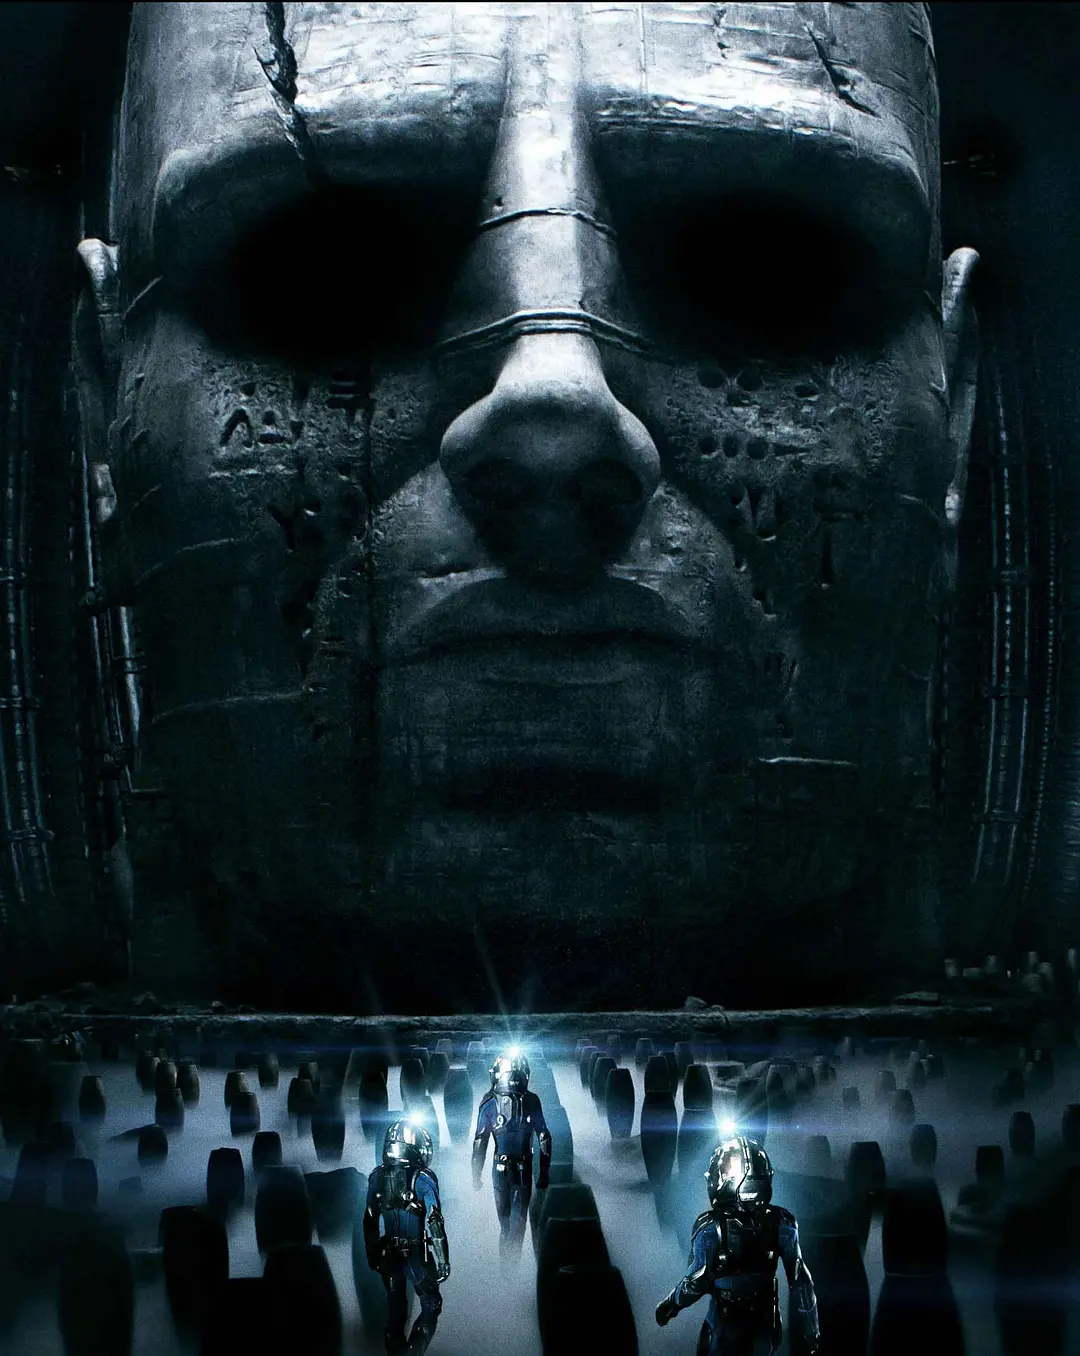
\includegraphics[width=\textwidth,height=0.62\textheight,keepaspectratio]{figures/fig02.png}
{\captiontext 电影《普罗米修斯》（Prometheus）中，当穿着宇航服、头戴头盔的探险队员们走入一座阴暗、神秘的巨大神殿时，看到了一座巨大的石雕人脸，这是“工程师”文明的遗迹。\par}
\end{center}

基于 \textbf{现成} 的科学知识、技术、工具并加以运用，“举国体制”虽然非常适合修筑长城与金字塔这样的 \textbf{大工程} ，但却无法孕育毕达哥拉斯、苏格拉底、牛顿、康德、高斯这类引领人类不断提升的伟大哲人与科学家，也不适合基础性、真创新性的学科，因此绝非万能药（panacea）。这是由于举国体制自身的工程性、实用性、功利性、运动性使其无法应对来自纯粹理性的普遍性与必然性的降维打击。

具体到个人，举国体制无法替代以真善美作为哲思与科研的终极目标而产生出的强大而持久的自驱力，以及在此目标指引下持续积累、反复练习、不断打磨出的小而美、小而精的优雅品质。在热火朝天的大干、快干中，个人的精力与潜力很容易被浪费、消耗，在激情中也难以维持宁静的心态并将理性与智慧发挥到极致。

另一方面，我们理性的运作与对于真理、真知的追求有其自身的规律与节奏，不可能永远与所谓的举国体制合拍，也不应当一直主动迎合。我们在自己研究方向上的科学探索、达成理解与完善技艺是一生一世的大事业，而举国体制所能支撑的某个方向与行业的热点大项目充其量也就不过十年。过度地适应与迎合，就会使自己陷入一会儿顺风顺水符合国家大趋势，一会儿又被体制与评价机制淘汰出局的量子迭加态。人生短暂，该拿什么作为我们人生与事业的核心来一以贯之，是每个人需要深刻思考与具体实践的大问题。

更进一步讲，总有一些根本的、绝对的、极度困难的学术与技术问题，就算没有国家的补贴、政策的支持、资本的助推、他人的认可，我们也一定要亲自去研究、摸索一番，乃至要把所有的死胡同都走过几遍之后，才能最终杀出一条血路。而这就是科研的第一推动力，也是“克己复礼”、“匹夫不可夺志”、“我欲仁，斯仁至矣”儒家精神的体现。引用阿德勒的话：“必须有人开始。即使别人不合作，那也与你无关。我的意见就是这样。应该由你开始，不用去考虑别人是否合作。”

\begin{classic}
《论语·卫灵公篇第十五 15.3》 子曰：「赐也，女以予为多学而识之者与？」对曰：「然，非与？」曰：「非也！予一以贯之。」

《论语·颜渊篇第十二 12.1》 颜渊问仁。子曰：「克己复礼，为仁。一日克己复礼，天下归仁焉。为仁由己，而由仁乎哉？」颜渊曰：「请问其目？」子曰：「非礼勿视，非礼勿听，非礼勿言，非礼勿动。」颜渊曰：「回虽不敏，请事斯语矣！」

《论语·子罕篇第九 9.26》 子曰：「三军可夺帅也，匹夫不可夺志也。」

《论语·述而篇第七 7.30》 子曰：「仁远乎哉？我欲仁，斯仁至矣。」
\end{classic}

\entrydate{2022.10.08}

\chapter{有教无类}

\begin{classic}
《论语·卫灵公篇第十五 15.39》 子曰：「有教无类。」

《论语·述而篇第七 7.22》子曰：「三人行，必有我师焉：择其善者而从之，其不善者而改之。」
\end{classic}

看到姜萍这样的人脱颖而出，且无论最终的比赛结果怎样、事件的真伪有无戏剧性反转，对于独立从事数学算法研究与开发、很多时候孤立无援的我来说，已着实是非常振奋人心了。

无论是出于平庸人内心的嫉妒，还是出于好奇心追求所谓的真相，质疑者虽无可厚非，但就像只为了获胜而辩论的辩手无法从争论中获得深层次的理解、共鸣与启迪，他们也无法从此人此事获得鼓舞与激励，从而有助于自我提升。孔子说的“攻乎异端，斯害也已”正是这个道理。当一个人内心对谁也不服气，对任何比他（无论是表面上还是实质上）优秀的人的第一反应都是抱以怀疑，这难道不是自大的表现么？人应当有对他人的卓越心悦诚服，并借机改进自己行动与习惯的意愿、能力和行动力。

鉴别姜萍有没有真才实学非常简单，只要有一个教授“屈尊”和姜萍面谈一次就水落石出了。但目前尚未看到有谁这么做。想来这已不是有没有伯乐的问题，而是连基本的任人唯贤、任人唯才都做不到。

事实上，姜萍发展的好坏与否毕竟与官员、教授的私利无关，甚至还可能对现有的高考制度、教育与学术体系产生解构的作用——因为当大众发现真才实学、学术自由、真正的创新与突破可以无需借助赢利性和世俗化的教育体系来外求，而终究只能靠个人求索来实现的时候，一直以来垄断学术资源与话语权的教育体系的权威性与光环便会削弱了。这样看来，没有哪个学校或专家愿意站出来打破惯例或做“出格”的事情也便很自然了。更何况，想要那个决定多少代人一生命运的机械的高考制度具有灵活性，本来也不是件容易的事。其前提是人心尚未堕落，且仍怀有理想与纯真，体制自身没有那么多腐败。以这个标准来看，中国还不具备这个条件。

无论是从微观的个人能否心怀敬佩的角度出发，还是从宏观体制是否清明、灵活的角度出发，反思大约一百年前英国皇家学会的数学家哈代发现、帮助拉马努金并与之合作结出硕果的感人事迹，才会发现要想践行与实现“伯乐”之难。同时，由“伯乐”这一典故也可略见我们的一大症结，即讲话与写作中的用词、造句都很漂亮，引据经典（非理论、理性的经典）亦看似博学，但是否真正能够做到以及做到了什么程度，则距离真善美的极至，或者退一步讲，距离人类历史已达到的高度相去甚远。但不管怎样，在现实与理想中，我们都需要有哈代与拉马努金。

\entrydate{2024.06.18}

\chapter{新年随想与寄语}

新年伊始往往是人们系统化回首过去和展望未来的好时机。就像不知是谁在这个新旧交替之际设置了一个颇具特殊意义的时间节点，正好适合品尝收获的甜美果实，并将行囊重新填满以信心和希望。

然而，“子在川上曰：逝者如斯夫”！时间本是如同河流，它相对于人短暂的一生来说，没有终始，更无预先划定的阶段与界限。虽然，因为每天的日出日落一直以来影响着人的作息，以“天”为单位的“日叁省吾身”是自然而合理的；然而所谓的“年”，便不过是地球绕太阳公转的周期。若以之作为人类生活的中、长期节律，在古代人类被庄稼“驯养”的农业社会倒还有一定的合理性，但到了如今工业化与信息化的经济时代，则只能是纯粹人为的设定，以至于既不具有时空绝对意义，也不具有个人生活与社会活动的现实意义了。

其实，两千多年前的孔夫子似乎也并无有关新年寄语或随想的只言片语。除了上文提到的把河流比作时间外，只闻他说过“君子无终食之间违仁”。对于谨小慎微的曾子，则是“如履薄冰”般地“日叁省吾身”。这样看来，我们的回顾、反省、规划、展望应当立体化地在短期、中期、长期多个维度上时时进行。每一分、每一秒以及做出的每一个选择均是极为重要的。与此同时，人的生命历程恰如一次无比漫长的星际旅行。立下的目标应当是一生的，从事的事业也是一生的。在这一生的求索历程中，每个人的人生有其自己的内在韵律和本征模式。而那些有待探索和发现的里程碑，也绝不会受到“年”的限制。

总之，新年之际的规划与展望其实已不再有什么特殊的意义，也更不应该成为一年中仅有的一次系统化自我整理的契机。由此送上我的2018新年寄语：

跳出时空的维度去了解你自己吧！发现你内在的人生韵律和本征模式！从现在开始，努力定位到属于你自己的那颗遥远的明星，开启一次精彩、历险且永不回头的星际航行！

\begin{classic}
《论语·子罕篇第九 9.17》 子在川上曰：「逝者如斯夫！不舍昼夜。」

《论语·里仁篇第四 4.5》 子曰：「富与贵，是人之所欲也，不以其道得之，不处也。贫与贱，是人之恶也，不以其道得之，不去也。君子去仁，恶乎成名。君子无终食之间违仁，造次必于是，颠沛必于是。」

《论语·泰伯篇第八 8.3》 曾子有疾，召门弟子曰：「启予足！启予手！诗云：『战战兢兢，如临深渊，如履薄冰。』而今而后，吾知免夫！小子！」

《论语·学而篇第一 1.4》 曾子曰：「吾日三省吾身，为人谋而不忠乎？与朋友交而不信乎？传不习乎？」
\end{classic}

\entrydate{2018.01.01}

\chapter{有朋自远方来}

《The Man Who Knew Infinity》书中提到Littlewood与Hardy的交往：

\begin{classic}
Littlewood had recently moved into rooms on D Staircase of Nevile’s Court. Pausing in the arched doorway at the staircase’s base, he could sight through the portico to the arches across the court framed within it. It was an arresting view—perhaps one reason he remained there for sixty-five years, until his death in 1977. From Hardy’s rooms, it was just nineteen steps down the winding stone staircase, then forty paces through the gate into Nevile’s Court and around to D Staircase. Yet normally the two men communicated by mail or college messenger and did not, in any case, routinely run off to confer with one another in person. And so, that winter evening in 1913, to let Littlewood know he wished to meet with him after Hall, Hardy sent word by messenger.
\end{classic}

二人的办公室虽然仅仅相距十九级台阶再加四十步，他们之间的交流却仍大多通过信件与信使，而不经常面谈。然而，这丝毫不妨碍他们之间的密切合作与深刻思想的碰撞交流。想来这就是我们常说但却鲜见的“君子之交”吧！而其中蕴含的精神与孔子和蘧伯玉的交往有着异曲同工之妙。

\begin{classic}
《论语·宪问篇第十四 14.25》 蘧伯玉使人于孔子，孔子与之坐而问焉。曰：「夫子何为？」对曰：「夫子欲寡其过而未能也。」使者出。子曰：「使乎！使乎！」
\end{classic}

可以看出，君子专注于“务本”，执著于对真善美的追求。因为“无终食之间违仁”，须臾不能离道，所以实再是没有功夫用来宴乐、交际。 这样一来，有限却深入的交流便显得弥足珍贵，偶尔的造访则更是成为铭记于心的乐事。然而，这样的朋友能否寻得，既须以自身的好学与修行为基础，也要看缘分。如有，则实属上天眷顾；没有，则仍需独自砥砺前行。

\begin{classic}
《论语·学而篇第一 1.2》 有子曰：「其为人也孝弟，而好犯上者，鲜矣；不好犯上，而好作乱者，未之有也。君子务本，本立而道生。 孝弟也者，其为仁之本与！」

《论语·里仁篇第四 4.5》 子曰：「富与贵，是人之所欲也，不以其道得之，不处也。贫与贱，是人之恶也，不以其道得之，不去也。君子去仁，恶乎成名。君子无终食之间违仁，造次必于是，颠沛必于是。」

《论语·季氏篇第十六 16.5》 孔子曰：「益者三乐，损者三乐。乐节礼乐，乐道人之善，乐多贤友，益矣。乐骄乐，乐佚游，乐宴乐，损矣。」

《论语·卫灵公篇第十五 15.17》 子曰：「群居终日，言不及义，好行小慧，难矣哉！」

《论语·学而篇第一 1.1》 子曰：「学而时习之，不亦说乎？有朋自远方来，不亦乐乎？人不知而不愠，不亦君子乎？」

《论语·子罕篇第九 9.30》 子曰：「可与共学，未可与适道；可与适道，未可与立；可与立，未可与权。」
\end{classic}

\entrydate{2022.03.14}

\chapter{道不同，不相为谋}

子曰：「道不同，不相为谋。」两个人即便在做同一个方向的研究，从事同一个领域的事业，因为各自有不同的终极目标、价值判准、做事风格、处世之道，想要达成一致根本不大可能，能寻得大体上的理解与认同就已实属不易了。人的一生虽然漫长，但十有八九遇到的也就是这么个情况。应对此局面的最佳态度倒也同样出自论语，即“刚毅木讷”。

所谓“木讷”，是出于两个人完全处在不同的频道上，难以相互理解并达成理想的一致，所以过多的讲述与解释也无非是浪费时间，甚至自取其辱。而之所以要做到“刚毅”，则是我们在不奢求有志同道合者的情况下，仍旧能够守得住原则，耐得住寂寞，既不会人云亦云，更不会借热门炒作。唯一要做的就是勤勉学习，敏于做事，闻道日肥。这难道不正是达成目标最高效的途径么？

\begin{classic}
《论语·宪问篇第十四 14.29》 子贡方人。子曰：「赐也，贤乎哉？夫我则不暇！」

《论语·卫灵公篇第十五 15.40》 子曰：「道不同，不相为谋。」

《论语·子罕篇第九 9.30》 子曰：「可与共学，未可与适道；可与适道，未可与立；可与立；未可与权。」
\end{classic}

\entrydate{2023.01.08}

\chapter{致友人的一封信}

以下截选自我曾写给友人的一封信。希望能在那些（尤其是走出学校后）一直坚持学术精神、热爱与追求技术的朋友心中产生一些共鸣。

很高兴看到你的心境得到改观，更平静地看待以前的人与事。人生总有些许无耐，每个人生均属不易——所以才需更加宽容！你若看过《永恒的爱》（Immortal Beloved）这部演艺贝多芬情感经历的电影，你会觉得我们要幸运得多。

根据你的描述，你目前的工作职位虽然号称是研究型，但每天实质上做的基本为重复性工作，而且还要在较短的周期内应对和解决诸多客户的问题。如此一来，工作不紧张才怪，不无聊才怪！其实，这也就是你的部门经理对你职位的定位，以及公司高层对你们部门工作性质的定位吧！再想想看，我们自己的出发点和立场何时与领导者的意愿真正是一致呢？他们考虑的是如何向上级交出成果，要快、要多，甚至可以因此忽略质量，无视技术；而我们自己则是希望所做的事情有技术价值和学术意义，并且能够怀有兴趣与热情去做自己渴望的研究工作，从而实现个人的发展以及对公司和社会的价值。可以看出，我们不过是一个被公司调用的棋子，有相当的时间可能不是为了技术本身而是为了一个无理头的决定或者是他人的颜面工作，谁又会考虑你个人的技术发展呢？所以，自己的路子还是要自己选择，自己来走，且应不断地调整。除非你真的到了很高的境界变得有话语权和影响力，这种调整的过程不会停止。

《大学》有云：

\begin{classic}
大学之道，在明明德，在亲民，在止于至善。知止而后有定，定而后能静，静而后能安，安而后能虑，虑而后能得。物有本末，事有终始，知所先后，则近道矣。
\end{classic}

《大学》章句为古之学者初学入门必读。由上面所摘首句即可看出，学者第一要务为明确自己的终极追求，即至善之地。若于为学伊始即立下此志，整个人生便会有所定向，才能做到心静如水，而宁静方能致远。对于我们来说，从走入科研大门的那一天开始，恐怕这样的立志就是颇为模糊的，甚于是缺失的。于是，在后续的研究与工作中，因为不明确自己“一定要做什么”以及“一定不能做什么”（后者尤为重要，它决定了你的底线），以至于从表面上看来我们做了一大堆项目，但却失去了对技术的专注与专业度，学术的素质与品味亦毫不见长 。长此以往，你就会发现离自己的初衷与梦想越来越远，可眼下的能力却又不足以说服他人支持你做想往的事情。这种理想与现实，理想与个人实力间的落差会让人陷入痛苦的泥淖。

想要从这样的泥淖中解脱确不是一件易事。毕竟，一个人在他现有的档次甚至是降级以做得风声水起乃至获得丰厚的利益是相对容易的。而要想让已成为社会人、成为为他人服务工具的自己再进阶一个层次则要付出百倍的努力。但无论怎样，你需要首先做到：始终不忘思忖自己的至善之地究竟在何处？其实，答案也许并不难得出：当你每每对于现状不满、失望，以至于情绪低落、琢磨着该怎么改变的时候，恰恰是上天向你暗示何处是属于你的至善之地的时候。只不过，由于我们已经习惯于目前的生活与工作环境，习惯于每天上下班的节奏与沿途的景致，以至于不愿意或者害怕有所改变——这就是积习的力量，也是懒惰的力量。其实，精神上的痛苦还不足以告诉我们自己真正想做的事吗？至少，这还不足以告诉我们哪些是自己不愿做的事吗？

有了终极目标，心即可归于安定与宁静。此时，即便是工作与生活还在变动，仍令人不满意，但心已不会随之纷乱。开始时，只能利用业余时间不断积累， 待时机成熟，则可全身心投入。统计一下：如果每天都能在一个方向上坚持积累2\textasciitilde{}3小时，经过8年即可达到10000小时。据网上的说法，此时就可以成为该领域的专家了。况且，由于我们对于原本想往的领域并非一窍不通，实际达成目标的时间可能还要更短。我想，这一点对于你也是适用的吧！

\entrydate{2016.12.04}

\chapter{断电小记}

前天晚上屋里突然断电。最先以为是入户电表跳闸——因为前一阵出现过同样的问题——然而，查看后才发现是屋内厨房地插的总闸跳掉了。于是，第二天跟物业预约了电工师傅上门检修。晚上六点半多，来了一位二十多岁的小伙子，我便开始和他一起在没有空调与风扇的闷热环境下忙到了八点半左右。其间，我们将厨房里所有的电源插座都拆开排查了一遍。他还穿过草丛，跳到小院里，寻找是否有从屋里引出到外面的插座。可结果，除了发现电气布线是一团糟外，根本没有可以快速解决的办法。看到小伙子浑身被汗水浸透，我的心里颇为过意不去。虽然问题并未得到解决，也没有更换任何部件，我仍旧给他微信转了维修费，从而稍感安慰。待小伙子走后，我顾不上吃饭，立即着手重新布置多个插排。到晚上十点钟，便将卫生间的电引出到了厨房，从而生活电器得以恢复使用U+3002至此，心里才觉得踏实，吃了点面包和水果当作夜宵。

可见，生活中总会遇到不如意的事。对此，应当以乐观的态度积极面对，将其看作是对自身的考验与磨炼。从而让自己像是沙漠中的红柳，总能够从困难与逆境中汲取有益的养分。同时，维修小伙子不怕脏、不怕苦的敬业精神也值得我虚心学习，并将这种精神迁移到数学研究上。

\begin{classic}
《论语·子罕篇第九 9.14》 子欲居九夷。或曰：「陋，如之何？」子曰：「君子居之，何陋之有！」

《史记·孔子世家第十七》 孔子曰：“回，诗云“匪兕匪虎，率彼旷野”。吾道非邪？吾何为於此？”
\end{classic}

\entrydate{2019.07.20}

\chapter{攻乎异端，斯害也已}

从网上看到一则消息，某人因为撰写了一篇药酒具有毒性的文章，而被派出所缉拿后关押了数月，后获得保释。若只是以此消息作为情景剧的素材而不追究事实真相，通过做一些虚拟假设来看看能否从中推导出为我们受用的结论，那么倒不妨将该事件设想为此人凭藉科学知识向奸商发起质疑和抨击，结果反倒因为商警勾结而含冤入狱。

基于这样的情景假设，我们便可以学到一点：最好通过做正确、积极、高尚的功业来吸引、影响和引导人，从而自然地令低劣产品难有市场生存空间，使污秽、恶劣的行径无藏匿之处；而不宜以举报、接发为己任，做针锋相对的事情，以至于在双方消耗的过程中虽然对恶势力也形成了一定的打击，但是良性的事业也没有因此得到培育和发展的机会。这种看似没有硝烟的斗争其实也是儒家智慧的体现，因为孔子有云：

\begin{classic}
《论语·为政篇第二 2.16》 子曰：「攻乎异端，斯害也己。」
\end{classic}

试想，孔子在春秋礼崩乐坏的时期，也并没有四处抨击当政者，更没有操戈厮杀于战场，而是用宣传礼乐教化的方式，培养了一大批人，在时间与地域的广大尺度上产生了深远的影响。世间的恶势力仅凭一个人、一群人、甚至一代人是无法肃清的，至多是拔除一些毒草，但仍无法撼动根基，更难以给人心、人性带来潜移默化的影响。所以更好的方式就是靠个人的积累、修炼、实践来起到“己欲立而立人”般的示范作用。之所以人心尚存很多恶，原因之一便是在这个“烂透了”的世界上，要做成一件从初衷开始，并从头至尾没有欺骗和原罪的正确的事业着实是“too damn hard”。人们因鲜见到有品味的成功案例与“以其道得之”的富贵，以至于失去信心，放弃甚至毁坏了人性向善的本质。

既然事已至此，我们就应当做出笃实而正确且完全合乎义的事业来向世界展示什么是真、善、美；要以此告诉世人我们每个人原本完全可以不必扭曲、憋屈、丧失自我地过活，也完全可以且应当享受和欣赏到货真价实、有质量、有品味、有美感的事物。即便终其一生也未能完成这样的事业，相信也会有志同道合者的接力。如此形成良性循环，善莫大焉。

\entrydate{2018.09.28}

\chapter{疫情之下《论语》带给我们的启示（一）}

新冠疫情的肆虐令 2020 年成为整个人类历史上极其不平凡的一年。直至今日，我们仍难以准确预期人类彻底战胜疫情的那一天。在这段艰难的岁月里，我们依然可以从《论语》中汲取着营养，将其渗透到生活的点滴之中。在《论语·公冶长》一篇中，孔子将他的志向总结为“老者安之，朋友信之，少者怀之”。曾子也说过“慎终追远，民德归厚矣”。这就教导我们对每一个具体的生命无分男女老幼，均应无比敬重和珍视。

\begin{classic}
《论语·公冶长篇第五 5.26》 颜渊、季路侍。子曰：“盍各言尔志？”子路曰：“愿车马、衣轻裘，与朋友共，敝之而无憾。”颜渊曰：“愿无伐善，无施劳。”子路曰：“愿闻子之志。”子曰：“老者安之，朋友信之，少者怀之。”

《论语·学而篇第一 1.9》 曾子曰：“慎终追远，民德归厚矣。”
\end{classic}

从《论语》中我们还可以看到，孔子所慎重的三件事中，“疾病”便占了其中一端。

\begin{classic}
《论语·述而篇第七 7.13》 子之所慎：齐，战，疾。
\end{classic}

这是因为，生命的安全与身体的健康是一个人得以持续行仁，在成为君子、止于至善的道路上坚持学习、慎思笃行、不断提升，并为国家与社会贡献价值的大前提。所以，我们必须予以高度的重视。这个时候，要了解、相信科学，以科学事实为依据，不要妄信和转发网上不靠谱的防疫或治病偏方。对此，《论语·乡党篇第十 10.16》也记载到，

\begin{classic}
康子馈药，拜而受之，曰：“丘未达，不敢尝。”
\end{classic}

孔子说过“危邦不入，乱邦不居”。所以，当下我们要尽一切可能避免去高危地区，尤其是社会动荡与政治混乱的国外。最好的做法就是待在自己当前生活与工作的地方，甚至是深居简出，自行居家隔离。这既是关照个人的健康，也是为他人和整个社会的生命安全负责。当然，在固守一地的日子里，生活未免有些单调。然而，只有“不仁者，不可以久处约”。只要我们以“行仁”作为精神核心，约束我们的言语、限制出行范围，反倒能够利用这段时间做一些深入、长远的思考，开展系统、专注的学习，好好修炼思想、端正态度、完善知识、提升技能。

\begin{classic}
《论语·泰伯篇第八 8.13》 子曰：“笃信好学，守死善道。危邦不入，乱邦不居，天下有道则见，无道则隐。邦有道，贫且贱焉，耻也，邦无道，富且贵焉，耻也。”

《论语·里仁篇第四 4.2》 子曰：“不仁者，不可以久处约，不可以长处乐。仁者安仁，知者利仁。”
\end{classic}

若我们与父母在不同的地方居住生活，则要尽量让彼此的距离不要相隔太远，从而无论疫情有何突发的状况，都能够相对方便地彼此相互照应、扶持。如果我们实在没有办法做到“不远游”，则应与父母保持比平时更加频繁的联系，随时报平安，让父母放心。

\begin{classic}
《论语·里仁篇第四 4.19》 子曰：“父母在，不远游，游必有方。”
\end{classic}

疫情之下，经济萧条、就业形势亦不乐观，这很容易让我们产生强烈的危机感和对未来职业发展的迷茫。这里，《论语》对我们的教导则是“人无远虑、必有近忧”。所以，我们应当具备长远的眼光，围绕核心技术、基础理论持续发力、做足准备，最终一定能从危机中发现社会发展的必然趋势、找到蕴藏于其中能够自我实现、服务国家的机会。

\begin{classic}
《论语·卫灵公篇第十五 15.12》 子曰：“人无远虑，必有近忧。”
\end{classic}

总之，只要我们在这段特殊的时期里好好珍惜时光、把握当下、修心修行，相信等到最终人类走出疫情阴霾的时候，我们应当从内到外、从思想到言语再到行动都会是焕然一新，获得的将是一个更好的自己。届时，经济也度过了它的低迷期，面对迫切需要基础与核心技术的国家、需要高端人才与工匠精神的市场，相信我们一定会大有所为。

\begin{classic}
《论语·子罕篇第九 9.13》 子贡曰：“有美玉于斯，韫而藏诸？求善贾而沽诸？”子曰：“沽之哉！沽之哉！我待贾者也！”
\end{classic}

\entrydate{2021.01.16}

\chapter{疫情之下《论语》带给我们的启示（二）}

肇始于2019年底的新冠疫情至今尚未过去。身在上海，我于2021年1月16日写“疫情之下《论语》带给我们的启示”这篇日记时，如同“隔岸观火”，只是在各种媒体上耳濡目染到与之相关的各种信息，生活上也不过是多了些洗手、戴口罩等个人防护方面的“繁琐”。而如今，新冠竟以燎原之势在上海肆虐，在实质上深刻影响与改变着每个人的生活、情绪、认知与思想。时过境迁，当我再翻看《论语》，发现依然能够找到一些语录，或许可以给处于封控下的我们带来思考、理解、接受、淡然。

\begin{classic}
《论语·为政篇第二 2.13》 子贡问君子。子曰：「先行其言，而后从之。」
\end{classic}

无论我们处于什么级别、做什么样的事情，都要谨言、慎行。先投入充足的工夫，把事情做到位，保证内在的质量与品味，而不只是徒有虚表。之后，再考虑是否公之于众。即便有自我宣传的必要，也要有所克制与保留——需知，谦逊乃做人的根基，亦应成为团队或者组织的风气。更何况，在面对类似当下的特殊情况时，形势瞬息万变，因一时的侥幸成功而马虎大意，往往会酿成大祸。

\begin{classic}
《论语·卫灵公篇第十五 15.17》 子曰：「群居终日，言不及义，好行小慧，难矣哉！」
\end{classic}

封控期间，整日居家，正是学习、修炼的好时候。此时，若在关注各种媒体讯息方面投入过多时间，则对己、对社会均无益处。不如趁这段时间好好提升自我，待疫情过后，将所学的知识与技能回馈社会。

\begin{classic}
《论语·为政篇第二 2.16》 子曰：「攻乎异端，斯害也己。」
\end{classic}

疫情期间，各种消息满天飞，真假难辨。即便信息确凿，有所谓的科学数据作支撑，发布者也往往是通过有意无意地捕捉片面真实来引导读者或观众忽略现实的复杂性而形成偏颇、谬误的整体性结论。若我们一直以来都是专心于学习、科研、开发、创作，其实也根本无暇顾及这些信息与观点的碎片，更没有必要和那些有悖于自己的感性观点或片面理性观点的人展开论战。这种口头上的一时酣畅淋漓往往毫无意义。

\begin{classic}
《论语·雍也篇第六 6.11》 子曰：「贤哉，回也！一箪食，一瓢饮，在陋巷，人不堪其忧，回也不改其乐。贤哉，回也！」
\end{classic}

将心思放在学习与德行的培养上，而不要在意吃喝是否种类丰富、做工精美。封控期间本来就物资调配困难，克制与收缩自己的欲望，不给他人增添麻烦。

\entrydate{2022.04.21}

% 论语学习与解读.tex
% Auto-generated from 感悟论语.odt by tools/odt_to_tex.py

\setpartplant{artwork/tangdi.png}
  {唐棣之华 · 《论语·子罕》}
  {未之思也，夫何远之有？}
  {《论语·子罕》}
  {论语学习与解读}
\part{论语学习与解读}

\chapter{论语入门读书顺序}

1. 傅佩荣《论语300讲》

2. 杨伯峻《论语译注》

3. 钱穆《论语新解》

4. 李泽厚《论语今读》

5. 朱熹《四书章句集注》论语部分

6. 傅佩荣《孔子辞典》

其中，傅佩荣《孔子辞典》与杨伯峻《论语译注》作为辞典随时查询。

\entrydate{2017.02.19}

\chapter{由《论语300讲》所感}

听过与读过傅佩荣教授在《论语300讲》中的解读后，我对《论语》有了更为真切的体会：不只是在自我管理与为人处事方面获益匪浅，更是促成了对人生方向的探索并使其逐渐明晰，以及对此方向锲而不舍的坚守与追寻。从孔子与其弟子的对话可以看出，古时读书人在求学伊始的第一要务是立志，是以修身、做人为本，而后才是求知——君子务本，本立而道生。由于他们能够不论在何时何地所作的抉择都是围绕着这个志向，因而较之今天的年轻人也就少有人生、事业与感情上的困惑。这种“择善固执”无需顾及外在环境与客观条件的优劣——饭疏食饮水，曲肱而枕，乐亦在其中矣；一箪食，一瓢饮，在陋巷，回也不改其乐，亦不会受制于时势命运——君子无终食之间违仁，造次必于是，颠沛必于是。而且，能够以毕生的付出和牺牲坚持走在通往至善与成为君子的道路上，直至最终“止于至善”。或者退一步说，即便这样的终极目标因天命而无法实现，然而正因为“朝闻道，夕可死矣”，所以纵然在刚刚意识到人生正途何在的时候便被上天剥夺了实现的机会，也同样是为时不晚、幸运且不留遗憾的。

以上便是傅佩荣在《论语300讲》中反复予以解读和强调的主旨思想：“人性向善，择善固执，止于至善”。这是值得我们每个中国人用心体会、慎思笃行和贯彻一生的精神内核。

\begin{classic}
《论语·学而篇第一 1.2》 有子曰：「其为人也孝弟，而好犯上者，鲜矣；不好犯上，而好作乱者，未之有也。君子务本，本立而道生。孝弟也者，其为仁之本与！」

《论语·卫灵公篇第十五 15.2》 在陈绝粮。从者病，莫能兴。子路愠见曰：「君子亦有穷乎？」子曰：「君子固穷，小人穷斯滥矣。」

《论语·述而篇第七 7.16》 子曰：「饭疏食，饮水，曲肱而枕之，乐亦在其中矣。不义而富且贵，于我如浮云。」

《论语·雍也篇第六 6.11》 子曰：「贤哉，回也！一箪食，一瓢饮，在陋巷，人不堪其忧，回也不改其乐。贤哉，回也！」

《论语·里仁篇第四 4.5》 子曰：「富与贵，是人之所欲也，不以其道得之，不处也。贫与贱，是人之恶也，不以其道得之，不去也。君子去仁，恶乎成名。君子无终食之间违仁，造次必于是，颠沛必于是。」

《论语·里仁篇第四 4.8》 子曰：「朝闻道，夕死可矣！」
\end{classic}

\entrydate{2018.02.06}

\chapter{《论语》的解读}

\begin{classic}
《论语·学而篇第一 1.1》 子曰：「学而时习之，不亦说乎？有朋自远方来，不亦乐乎？人不知而不愠，不亦君子乎？」
\end{classic}

以上《论语 学而》第一章大家已是耳熟能详了。记得这一章连同“学而不思则罔，思而不学则殆”等曾经被选入我初中一年级的语文课本。虽然这一章看似浅显易懂，但是否能够理解到位乃至切实践行，就不好说了。仅以“学而时习”中的“时”字为例，一般人望文生义，会将其理解为“时常”，也就像是中小学生的定期复习那样，要想学得好，就要不断反复。这样的理解对于以其四分之一至三分之一人生投入应试教育的广大学生无疑有着“重大”的教益，因此也颇得老师与家长的认可。

相比之下，大师的解读便没有那么功利了。例如，钱穆在《论语新解》中对“时”字给出了三种解释：

\begin{itemize}
\item 指年岁。例如“古人六岁始学识字，七八岁教以日常简单礼节，十岁教书写计算，十三岁教诗歌舞蹈”。
\item 指季节。古人春夏学诗乐弦歌，秋冬学书礼射猎。
\item 指一日中的晨夕。
\end{itemize}

可以看出，钱穆的解释采用的是“时”字的字面意思，即“时间”，只不过尺度不同罢了。看过这样的解释，便会对古人学习的内容、流程、习惯有所了解，相当于掌握了时代背景。

而傅佩荣教授在其《论语三百讲》中则将“时”解释为“恰当的时候”。意即对学所学的礼仪、射猎等知识和技术、技能，需要在合适的时候加以练习。这是因为，孔子所传授的内容并非可以独立于现实的纯粹理论和逻辑推理，而是需要在生活中加以实践和反省的人生学问与哲学，例如人生志向的确立、原则的坚守、孝敬的践行。它们都是依赖于环境与客观条件的，甚至取决于一定的机缘。

由以上可以看出，对于《论语》的学习与理解，普通人与大师有所不同，大师与大师之间也不尽相同，正所谓仁者见仁、智者见智。对此，我认为不必拘泥和固执于所谓的权威、原意、真意，而应以能够对书中的词汇、内容加以发挥、引申，从而触发个人感悟并由感悟落实到积极行动为好。若从负面的例子来看，经过几千年的演变，如今人们头脑中的儒家思想早已不是原本的样子，尤其是掺入了许多僵化、教条甚至是腐朽的观念，其影响还流传得相当广。但事实上，这些错误、片面的理解根本不是孔子最初的思想。这样看来，《论语》在事实上已经成为了囊括不同理解的统一形式。为此，为什么不能用提炼数学理论的方式来看待、处理《论语》？即，将其当作由抽象性符号构建的框架，用以容纳来自不同视角的解读、阐释。同时，要求这些阐释必须具有积极与正面的意义，深刻而丰富内涵，既可以从宏观把握、又可以指导细处的实践。由此，《论语》将成为不断完善、深化的思想体系，无论对于个人的修身、立志，还是对于优秀民族性格的构建，都是大有裨益的。

\entrydate{2017.07.08}

\chapter{《论语·学而1.1》解读}

《论语》的编排以“学而”作为首篇，以“学而时习”开宗明义，可以看出儒家对于“学习”的重视。其中，“时”是指“在适当的时候”（杨伯峻《论语译注》 P1）或“时常”、“时时”（朱熹《四书章句集注》 P47，谢氏曰：「无时而不习」）。傅佩荣(《论语300讲》上册 P1）则进一步强调学习要把握时机，在适当的时候去实践。当然，这里的学习不仅指科学知识，还应拓展到生活、社会、待人、做事等诸多方面，涉及生命、人生的大学问、大智慧。它们彼此相辅相成，是贯穿一个人毕生追求君子之道、推己及人、止于至善的基石。

具体说来：

\begin{itemize}
\item 在学习与研究方面，要做好详细的计划，这样才能做到有规律的时常复习、练习，而不是浅尝辄止、一曝十寒。同时，要注意不能避重就轻，光挑那些相对容易的科目，例如，偏向实用而忽略理论；或是见异思迁，只选那些愉悦感观的材料，例如诗词歌赋而非思辩哲学。随着年龄的增长，我们积累的知识与技能越来越多，再向其中系统性地增添大量新内容也会愈加困难。此时要想做到“月无忘其所能”，就必须增加复习的次数与频率。
\item 在行仁与孝敬方面，需要把握恰当的时机。在每一次与家人的沟通交流中，在待人接物中，在职业发展与人生选择中，珍惜现实提供的机会，回顾并应用从论语中学到的原则。
\item 在个人修行方面，要在恰当的时候，例如遇到倦怠、松懈、怯懦、灰心等个人性格弱点出现的情况时，跳出自己的舒适圈，与坏习惯做斗争。
\end{itemize}

由此推想开来：能将学习本身定位为人生的基本要素，便不会将其当作追名逐利的敲门砖。如果一个人发自内心地重视学习，其必然会坚持真理，不盲信、不盲从，拥有超越评价体系（游戏规则）的独立思考，做事亦会有原则和底线。将学习放在首位，才可以始终怀有童心、初心，以开放的胸怀了解、接纳新事物，才能做到苟日新、日日新。以学习作为终极目标，才能真正做到慎思笃行，始终走在择善固执、止于至善的道路上。能成就这样的自我，便是做到了孔子所说的“君子不器”。而且同样地，亦不会把他人当作工具。所谓“己欲立而立人，己欲达而达人”、“君子成人之美”是也。而这些均与学习是密不可分的。

有了书本上和实践中笃实的学习乃至形成深厚的积淀，志同道合的朋友相聚时，才会“以文会友，以友辅仁”。彼此交流的是关于永恒真理的理解与感悟。而那些酒桌上常见的热烈与殷勤，日常相处的如胶似漆，充其量只能算是小人的“同而不和”罢了。（注：《论语》中的小人不含贬义，只是用来形容一个人的言行、心智仍像是孩童，就像是武志红提出的“巨婴”概念）人生往往难觅投缘的好友，更难觅“爱真理胜过吾师”的知己。这样看来，“有朋自远方来”的情境岂不是一大快乐？

“学而”的最后一部分，“人不知而不愠，不亦君子乎”，讲的是宠辱不惊的人生境界。知音难觅，而误解司空见惯。能够形成这样的豁达，有赖于不断的学习和实践来给自己提供足够的智慧和修养。不仅如此，孔子亦说过“不患人之不己知，患己之不能也”，由是观之，“人不知而不愠”恰恰又是鞭策自我更进一步虚心与深入学习的动力。

\begin{classic}
《论语·学而篇第一 1.1》 子曰：「学而时习之，不亦说乎？有朋自远方来，不亦乐乎？人不知而不愠，不亦君子乎？」

《论语·为政篇第二 2.12》 子曰：「君子不器。」

《论语·雍也篇第六 6.30》 子贡曰：「如有博施于民，而能济众，何如？可谓仁乎？」子曰：「何事于仁，必也圣乎！尧舜其犹病诸！夫仁者，己欲立而立人，己欲达而达人。能近取譬，可谓仁之方也已。」

《论语·颜渊篇第十二 12.16》 子曰：「君子成人之美，不成人之恶。小人反是。」

《论语·颜渊篇第十二 12.24》 曾子曰：「君子以文会友，以友辅仁。」

《论语·子路篇第十三 13.23》 子曰：「君子和而不同，小人同而不和。」

《论语·学而篇第一 1.16》 子曰：「不患人之不己知，患不知人也。」

《论语·宪问篇第十四 14.30》 子曰：「不患人之不己知，患其不能也。」
\end{classic}

\entrydate{2017.07.08}

\chapter{《关睢》与“兴”的表达手法}

\begin{classic}
“关关雎鸠，在河之洲”，毛传：“兴也。”所谓“兴”，可以说是引起话题，或者说是由景引起情。这景与情的碰合多半是诗人当下的感悟，它可以是即目，也不妨是浮想；前者是实景，后者则是心象。但它仅仅是引起话题，一旦进入话题，便可以放过一边，因此“兴”中并不含直接的比喻，若然，则即为“比”。——《诗经别裁》摘录
\end{classic}

诗经多用兴的手法，而之后古人说话也多引用诗经中的句子来“兴”起自己要表达的意思，从而使表达变得委婉文雅。比如，两国之间外交官的官方对话必要以诗经作为引子，而且还会奏乐——因为诗经原本都是可以唱的。古代人说话不会太直白的这一特点也值得今人借鉴。比如，孔子的学生端木赐想要知道孔子是否想从政，直接问太唐突，他便说木匣中有一美玉，请问是将其卖掉呢，还是自己珍藏呢？端木赐，名子贡，是孔子门下言语科排名第一的学生，口才极好，由此可见一斑。“兴”的表达方式也可见于文人将其志寄寓于植物。如松柏于岁寒中后凋，竹之坚韧正直。

对于《关睢》的理解也应借助“兴”升华到更高的层次与境界。即，将“窈窕淑女”引申为我们的终极理想、至善之地，而借君子“寤寐思服”、“辗转反侧”的“好逑”兴起自己对志向矢志不渝的追求。这样，一首诗便不仅仅是具有美感的艺术，更是对我们人生中的关键因素，如立志、践行、时穷节乃见、不轻易放弃，有着重要的现实推动意义。而前提是需要提升我们自身的领悟能力，使其能够与古人的优秀思想对接。

\entrydate{2017.01.21}

\chapter{回归文字的原义}

对于《论语》、《诗经》等作品所蕴含道理的理解仅停留于字面显然是不行的。但若拘泥于引申后正确、标准的现代含义也仍旧不足。比如，今晨醒来后脑海浮现出了《论语 学而第一 1.15》中的那句“如切如磋，如琢如磨”（源于《诗经 卫风 淇奥》）。由于对这句话已经耳熟能详，甚至都产生免疫力了，所以对于“切磋琢磨”四个字的第一感觉便是我们常用的引申义，即，通过不断打磨和完善自我，以追求君子的完美境界。这样的理解固然不错，但却丧失了文字原本鲜活的形象和生动的意义。因而，就像是只有法律条文的约束但缺乏宗教情怀的感召与启发一样，如此的理解对于指导实践、激励个人立志、促进自我提升的作用反倒不那么显著与深刻了。

周振甫《诗经译注》中对“切磋琢磨”的解释为：“治骨曰切，治象牙曰磋。治玉曰琢，治石曰磨”。若将这几件工作的具体形象呈现出来，就会发现将其用于形容君子择善固执的提升过程与止于至善的终极境界是多么地恰如其分了。可以想象，一位技艺卓越、一丝不苟的工匠，他那经过了深思熟虑后的每一刀切下去都是无比地稳定沉着、精准无误。骨角玉石在他每一次小心翼翼但又娴熟的雕琢与打磨后虽只落下那么一点点亮晶晶的粉屑，但如此经过成百上千次地反复后，外形、质地、纹理上细致入微的变化终于累积出了巧夺天工般的维妙维肖与圆润细腻。很显然，好习惯由个别到完整体系的逐步养成，以及最终君子品性的塑成，都不是一蹴而就的，都是通过这么一点点地精雕细琢，由无数个微小细节积累出来的。每一次的提升与改进虽然微小，但却无比扎实，毫无后顾之忧。这便是任何人想要臻于完美所应遵循的一般过程。任何有悖于此的浮躁、急切、贪心、自以为是，无论能够从中得到多少现实的效果与回报，都是没有意义且难以持久的。

最后，让我们再回顾一下《论语 学而第一 1.15》的原文和杨伯峻的翻译吧！

原文：

\begin{classic}
子贡曰：“诗云：‘如切如磋，如琢如磨’，其斯之谓与？”子曰：“赐也，始可与言诗已矣，告诸往而知来者。”
\end{classic}

翻译：

\begin{classic}
子贡说：“诗经上说：‘要像对待骨、角、象牙、玉石一样，先开料，再糙锉，细刻，然后磨光。’那就是这样的意思吧？”孔子道：“赐呀，现在可以同你讨论诗经了，告诉你一件，你能有所发挥，举一反三了。”

《论语·学而篇第一 1.15》 子贡曰：「贫而无谄，富而无骄，何如？」子曰：「可也，未若贫而乐，富而好礼者也。」子贡曰：「诗云：『如切如磋，如琢如磨』，其斯之谓与？」子曰：「赐也，始可与言诗已矣，告诸往而知来者。」
\end{classic}

\entrydate{2018.07.29}

\chapter{性相近，习相远}

\begin{classic}
《论语·阳货篇第十七 17.2》 子曰：「性相近也，习相远也。」
\end{classic}

性相近，是指人性大都具有欣赏、向往、追求真、善、美的倾向。其中，“真”代表科学与理性，“善”为道德与正义，“美”是艺术性的升华（exaltation）。这三者并非泾渭分明，而是各自均在一定程度上包含其他成分，相辅相成。这种人性的倾向并不一定最终达成事实上的必然，仅代表了人性的 \textbf{初值} 和今后发展的一种可能。因此，由于每个人后天学习、经验、磨炼、成长的路径不同，志向与努力的程度也不同，并由此导致言语、思想、行动、习惯、命运的差异，最终渐行渐远，鲜有殊途同归。这便是《论语·子罕篇第九 9.30》所讲的：

\begin{classic}
子曰：「可与共学，未可与适道；可与适道，未可与立；可与立，未可与权。」
\end{classic}

本章“习相远”中的“习”指人的习惯、习性。同时，我们也还记得，《论语·学而篇第一 1.1》中孔子讲“学而时习”，《论语·学而篇第一 1.4》中曾子讲“传不习乎”，其中的“习”均指练习、实践。若将其与本章的“习相远”对照，则可看出不同的人在后天学习与实践上花费的工夫与修炼的程度往往存在很大差异。这样一来，“三人行必有我师”，我们总能在某方面找到让自己学习、提升的榜样，也会发现让自己引以为戒的反面教材。因此，“习相远”这一客观事实，有助于我们形成“见贤思齐，见不贤而内自省”的动力。

\entrydate{2023.04.19}

\chapter{故作高深}

\begin{classic}
《论语·宪问篇第十四 14.35》子曰：「莫我知也夫！」子贡曰：「何为其莫知子也？」子曰：「不怨天，不尤人，下学而上达。知我者，其天乎！」
\end{classic}

虽然孔夫子与苏格拉底同属人类文明轴心时代的四大圣哲，其与各自弟子对话、探讨的方式却完全不同。前者故弄玄虚、故作高深、曲折逶迤。后者分类定义、逻辑严谨、平等透彻。由此，在探求真理、求知除昧的层面，他们对于人类文明的影响与推动效果迥异。

孔夫子与弟子们的谈话方式给后世直至今日的中国人在为政、治学、实业等诸多领域带来了负面影响。看似高深莫测、自我感觉真诚而良好，但往往实际说的是大话、空话、漂亮话（即邓晓芒老师所说的自欺）。虽然字句对仗工整，但内在逻辑链条实则很短，更无所谓复杂体系的构建；概念没有明确定义，相互重叠且整体上不完备。在教与学的具体实践上，老师的讲解、讲义、教材鲜有深入、透彻、酣畅淋漓者。学生中自由探讨，大胆质疑，求真理而非褒吾师者亦不多。

论语中类似打哑谜的对话还有：

\begin{classic}
《论语·八佾篇第三 3.13》 王孙贾问曰：「与其媚于奥，宁媚于灶，何谓也？」子曰：「不然，获罪于天，无所祷也。」

《论语·述而篇第七 7.15》 冉有曰：「夫子为卫君乎？」子贡曰：「诺，吾将问之。」入曰：「伯夷、叔齐何人也？」曰：「古之贤人也。」曰：「怨乎？」曰：「求仁而得仁，又何怨？」出曰：「夫子不为也。」
\end{classic}

\entrydate{2023.05.07}

\chapter{《论语》中的生动画面}

\begin{classic}
《论语·乡党篇第十 10.27》 色斯举矣，翔而后集。曰：「山梁雌雉，时哉时哉！」子路共之，三嗅而作。
\end{classic}

这一章描绘出了一幅生动的画面：深秋时节，孔子与弟子们在层林尽染的山间漫步。道旁是潺潺的溪流，溪水清冽。一群雌雉在桥边觅食，时而飞起散开，时而降落聚集。在这清冷、萧索的天地之间，孔子的头脑清醒、精神振奋，有感于大自然中的鸟兽生灵，获得了君子“时哉”的启发：君子应把握时机，顺应时机，无可无不可，但一切又应以坚守的原则和远大的终极理想为前提。难怪，孟子后来将孔子称作“圣之时者也”。闻过则喜的子路则在内心暗暗记下了老师的感悟，以示受教的谢意——这正是他的可爱与纯真之处。

\begin{center}
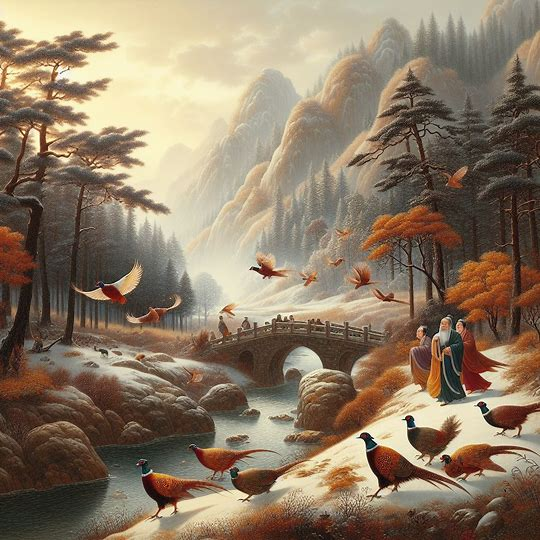
\includegraphics[width=\textwidth,height=0.62\textheight,keepaspectratio]{figures/fig03.png}
\end{center}

\entrydate{2023.09.18}

\chapter{克己复理}

\begin{classic}
《论语·颜渊篇第十二 12.1》颜渊问仁。子曰：「克己复礼，为仁。一日克己复礼，天下归仁焉。为仁由己，而由仁乎哉？」颜渊曰：「请问其目？」子曰：「非礼勿视，非礼勿听，非礼勿言，非礼勿动。」颜渊曰：「回虽不敏，请事斯语矣！」
\end{classic}

将此章中的“克己复礼”改为“克己复理”就对了！

“克己”的意思是“自己能够”，即调动自己的主观能动性，将天赋、潜力、勤奋发挥到极致。英文里对应的表述则是take your initiatives：

\begin{classic}
take your initiatives (initiative [Oxford Advanced Learner] n. the ability to decide and act on your own without waiting for sb to tell you what to do.)。
\end{classic}

“复理”与“复礼”的意思正好相反，是去除人与人之间的等级、贵贱差异——例如在学术领域就是要消除学阀与青年学者、大团队与小团体在项目申请与评审上的潜在不公平性——代之以在理性的指引下，基于具有普遍性与必然性的原则思考、分析、表达、做事。“使我们自己能够去做”而不是“在体制与政策的指引下去做”，从中体现出的就是自由、平等、去中心化、去权威化的精神。“独立之精神、自由之思想”，这是做学问的根本。

“克己”是从我们自身方面着眼，始终努力实践的基本原则。“复理”则是从外在环境与体制来说的，我们个人便很难对其施加影响以改变方向。环境好的时候，顺水行舟，邦有道则谷。环境不好的时候，仍应择善固执，避免成为体制与时代的牺牲品。无论外界如何变化，都应做出一些或者哪怕一点点能够真正发人深省、震撼人心、引领时代与推动人类的成果、产品、佳作。我想只有如此，才能无愧于清华“立德立言，无问西东”的精神。

\entrydate{2024.02.04}

% 附录一.tex
% Auto-generated from 感悟论语.odt by tools/odt_to_tex.py

\setpartplant{artwork/pine.png}
  {松柏}
  {诗三百，一言以蔽之，曰：思无邪。}
  {《论语·为政》}
  {附录}
\part*{附录一：《论语》章句分类}
\addcontentsline{toc}{part}{附录一：《论语》章句分类}

《论语》编排孔子与其弟子语录既非按时间顺序，亦未分门别类。于是，对于初读者来说，一下子接受这么多具有丰富内涵的经典，便难以在一时之间形成易于理解、能与自身经验形成映照的内在逻辑联系与思想体系。而若想有计划地将这些思想的瑰宝逐步实践就会更为零乱无序。这就像用无底桶或网孔很大的渔网捕鱼一样徒劳无功。即便孔子以“仁”来“一以贯之”，但这已是高度浓缩的概括与抽象，对于理解与实践也没有太大的作用。因此，我们需要用自己的逻辑思考去编织一道细密的网，从《论语》这个富含宝藏的大海中“打捞”出主要思想，对其规纳、组织、分类，并落实到自己的实践与生活习惯中。这样，每当我们临事而迷或对生活有所怨愤时，《论语》中相应的篇章便会自然在脑海中浮现，从而给我们以精神力量去坚守自己的原则。

以下是我对《论语》中重要且有切身感触的篇章所进行的分类整理。这个分类当是持续更新与不断完善的。即，随着自己理解的深入，体会的丰富，实践的笃实，知与行不断地交互、促进，其亦将会更加地合理与完整；每一类中的章句也会逐步地扩充直至完善；对于每一章句的注释与体会记录亦会不断地充实。同时，需要说明的是，由于《论语》的内涵通常涉及多个层面，同一章句可能会出现于多个分类中。

\chapter{志向与人生追求}

傅佩荣教授所总结的“人性向善、择善固执、止于至善”的三步曲。对此，不得不提及《大学》的首句：

大学之道 ，在明明德，在亲民，在止于至善。知止而后有定，定而后能静，静而后能安，安而后能虑，虑而后能得。物有本末，事有终始。知所先后，则近道矣。古之欲明明德于天下者，先治其国；欲治其国者，先齐其家；欲齐其家者，先修其身；欲修其身者，先正其心；欲正其心者，先诚其意；欲诚其意者，先致其知；致知在格物。物格而后知至，知至而后意诚，意诚而后心正，心正而后身修，身修而后家齐，家齐而后国治，国治而后天下平。自天子以至于庶人，壹是皆以修身为本。其本乱而末治者否矣。其所厚者薄，而其所薄者厚，未之有也。

（里仁第四 4.8）子曰：“朝闻道，夕可死矣。”

（子罕第九 9.26）子曰：“三军可夺帅也，匹夫不可夺志也。”

\chapter{逆境中的坚守}

（学而第一 1.14）子曰：“君子食无求饱，居无求安，敏于事而慎于言，就有道而正焉，可谓好学也已。”

（卫灵公第十五 15.2）在陈绝粮，从者病，莫能兴。子路愠见曰：“君子亦有穷乎？”子曰：“君子固穷，小人穷斯滥矣。”

（史记·孔子世家）孔子知弟子有愠心，乃召子路而问曰：“诗云“匪兕匪虎，率彼旷野”。吾道非邪？吾何为於此？”子路曰：“意者吾未仁邪？人之不我信也。意者吾未知邪？人之不我行也。”孔子曰：“有是乎！由，譬使仁者而必信，安有伯夷、叔齐？使知者而必行，安有王子比干？”子路出，子贡入见。孔子曰：“赐，诗云“匪兕匪虎，率彼旷野”。吾道非邪？吾何为於此？”子贡曰：“夫子之道至大也，故天下莫能容夫子。夫子盖少贬焉？”孔子曰：“赐，良农能稼而不能为穑，良工能巧而不能为顺。君子能脩其道，纲而纪之，统而理之，而不能为容。今尔不脩尔道而求为容。赐，而志不远矣！”

子贡出，颜回入见。孔子曰：“回，诗云“匪兕匪虎，率彼旷野”。吾道非邪？吾何为於此？”颜回曰：“夫子之道至大，故天下莫能容。虽然，夫子推而行之，不容何病，不容然後见君子！夫道之不脩也，是吾丑也。夫道既已大脩而不用，是有国者之丑也。不容何病，不容然後见君子！”孔子欣然而笑曰：“有是哉颜氏之子！使尔多财，吾为尔宰。”

（述而第七 7.16）子曰：“饭疏食饮水，曲肱而枕之，乐亦在其中矣。不义而富且贵，于我如浮云。”

（雍也第六 6.11）子曰：“贤哉，回也！一箪食，一瓢饮，在陋巷，人不堪其忧，回也不改其乐。贤哉，回也！”

（里仁第四 4.5）子曰：“富与贵，是人之所欲也；不以其道得之，不处也。贫与贱，是人之所恶也；不以其道得之，不去也。君子去仁，恶乎成名？君子无终食之间违仁，造次必于是，颠沛必于是。”

（阳货第十七 17.7）子曰：“不曰坚乎，磨而不磷；不曰白乎，涅而不缁。”

\chapter{学与教}

（学而第一 1.1）子曰：“学而时习之，不亦说乎？有朋自远方来，不亦乐乎？人不知，而不愠，不亦君子乎？”

（为政第二 2.11）子曰：“温故而知新，可以为师矣。”

（为政第二 2.15）子曰：“学而不思则罔，思而不学则殆。”

（为政第二 2.16）子曰：“攻乎异端，斯害也已。”

（为政第二 2.17）子曰：“由！诲女知之乎！知之为知之，不知为不知，是知也。”

（公冶长第五 5.15）子贡问曰：“孔文子何以谓之‘文’也？”子曰：“敏而好学，不耻下问，是以谓之‘文’也。”

（述而第七 7.8）子曰：“不愤不启，不悱不发。举一隅不以三隅反，则不复也。”

（卫灵公第十五 15.31）子曰：“吾尝终日不食，终夜不寝，以思，无益，不如学也。”

（卫灵公第十五 15.39）子曰：“有教无类。”

（季氏第十六 16.9）孔子曰：“生而知之者，上也；学而知之者，次也；困而学之，又其次也；困而不学，民斯为下矣。”

（阳货第十七 17.8）子曰：“由也！女闻六言六蔽矣乎？”对曰：“未也。”“居！吾语女。好仁不好学，其蔽也愚；好知不好学，其蔽也荡；好信不好学，其蔽也贼；好直不好学，其蔽也绞；好勇不好学，其蔽也乱；好刚不好学，其蔽也狂。”

（阳货第十七 17.9）子曰：“小子何莫学夫诗？诗，可以兴，可以观，可以群，可以怨。迩之事父，远之事君；多识于鸟兽草木之名。”

\chapter{做事与说话}

（学而第一 1.14）子曰：“君子食无求饱，居无求安，敏于事而慎于言，就有道而正焉，可谓好学也已。”

（为政第二 2.18）子张学干禄。子曰：“多闻阙疑，慎言其余，则寡尤；多见阙殆，慎行其余，则寡悔。言寡尤，行寡悔，禄在其中矣。”

子贡为言语科第二，以下摘录其语录：

（学而第一 1.15）子贡曰：“贫而无谄，富而无骄，何如？”子曰：“可也；未若贫而乐，富而好礼者也。”子贡曰：“诗云：‘如切如磋，如琢如磨。’其斯之谓与？”子曰：“赐也，始可与言诗已矣，告诸往而知来者。”

（述而第七 7.15）冉有曰：“夫子为卫君乎？”子贡曰：“诺；吾将问之。”入，曰：“伯夷、叔齐何人也？”曰：“古之贤人也。”曰：“怨乎？”曰：“求仁而得仁，又何怨？”出，曰：“夫子不为也。”

（子罕第九 9.13）子贡曰：“有美玉于斯，韫椟而藏诸？求善贾而沽诸？”子曰：“沽之哉！沽之哉！我待贾者也。”

（乡党第十 10.1）孔子于乡党，恂恂如也，似不能言者。其在宗庙朝廷，便便言，唯谨尔。

（乡党第十 10.2）朝，与下大夫言，侃侃如也；与上大夫言，訚訚如也。君在，踧踖如也，与与如也。

（子张第十九 19.21）子贡曰：“君子之过也，如日月之食焉：过也，人皆见之；更也，人皆仰之。”

（子张第十九 19.23）叔孙武叔语大夫于朝曰：“子贡贤于仲尼。”子服景伯以告子贡。子贡曰：“譬之宫墙，赐之墙也及肩，窥见室家之好。夫子之墙数仞，不得其门而入，不见宗庙之美，百官之富。得其门者或寡矣。夫子之云，不亦宜乎！”

（子张第十九 19.24）叔孙武叔毁仲尼。子贡曰：“无以为也！仲尼不可毁也。他人之贤者，丘陵也，犹可逾也；仲尼，日月也，无得而逾焉。人虽欲自绝，其何伤于日月乎？多见其不知量也。”

颜渊为德行科第一，以下摘录其语录：

（子罕第九 9.11）颜渊喟然叹曰：“仰之弥高，钻之弥坚。瞻之在前，忽焉在后。夫子循循然善诱人，博我以文，约我以礼，欲罢不能。既竭吾才，如有所立卓尔。虽欲从之，末由也已。”

诗经的引用能让言语更加文雅与委婉，摘录相关章句如下：

（八佾第三 3.8）子夏问曰：“‘巧笑倩兮，美目盼兮，素以为绚兮。’何谓也？”子曰：“绘事后素。”曰：“礼后乎？”子曰：“起予者商也！始可与言诗已矣。”

（泰伯第八 8.3）曾子有疾，召门弟子曰：“启予足！启予手！诗云：‘战战兢兢，如临深渊，如履薄冰。’而今而后，吾知免夫！小子！”

\chapter{修养与品质}

（学而第一 1.8）子曰：“君子不重，则不威；学则不固。主忠信。无友不如己者。过，则勿惮改。”

（学而第一 1.16）子曰：“不患人之不己知，患不知人也。”

（里仁第四 4.14）子曰：“不患无位，患所以立。不患莫己知，求为可知也。”

（里仁第四 4.17）子曰：“见贤思齐焉，见不贤而内自省也。”

（宪问第十四 14.30）子曰：“不患人之不己知，患其不能也。”

（雍也第六 6.18）子曰：“质胜文则野，文胜质则史。文质彬彬，然后君子。”

（子罕第九 9.28）子曰：“岁寒，然后知松柏之后凋也。”

（为政第二 2.24）子曰：“非其鬼而祭之，谄也。见义不为，无勇也。”

（季氏第十六 16.13）不学诗，无以言。不学礼，无以立。

（尧曰第二十 20.3）孔子曰：“不知命，无以为君子也；不知礼，无以立也；不知言，无以知人也。”

（雍也第六 6.3）哀公问：“第子孰为好学？”孔子对曰：“有颜回者好学，不迁怒，不贰过。不幸短命死矣，今也则亡，未闻好学者也。”

（子罕第九 9.29）子曰：“知者不惑，仁者不忧，勇者不惧。”

（子路第十三 13.21）子曰：“不得中行而与之，必也狂狷乎！狂者进取，狷者有所不为也。”

（子路第十三 13.27）子曰：“刚、毅、木、讷，近仁。”

（卫灵公第十五 15.24）子贡问曰：“有一言而可以终身行之者乎？”子曰：“其恕乎！己所不欲，勿施于人。”

\chapter{君子与小人之别}

（为政第二 2.14）子曰：“君子周而不比，小人比而不周。”

（里仁第四 4.16）子曰：“君子喻于义，小人喻于利。”

（述而第七 7.37）子曰：“君子坦荡荡，小人长戚戚。”

（颜渊第十二 12.16）子曰：“君子成人之美，不成人之恶。小人反是。”

（颜渊第十二 12.16）季康子问政于孔子曰：“如杀无道，以就有道，何如？”孔子对曰：“子为政，焉用杀？子欲善而民善矣。君子之德风，小人之德草。草上之风，必偃。”

（子路第十三 13.20）子贡问曰：“何如斯可谓之士矣？”子曰：“行己有耻，使于四方，不辱使命，可谓士矣。”曰：“敢问其次。”曰：“宗族称孝焉，乡党称弟焉。”曰：“敢问其次。”曰：“言必信，行必果，硁硁然，小人哉！抑亦可以为次矣。”

（子路第十三 13.23）子曰：“君子和而不同，小人同而不和。”

（子路第十三 13.25）子曰：“君子易事而难说也。说之不以道，不说也；及其使人也，器之。小人难事而易说也。说之虽不以道，说也；及其使人也，求备焉。”

（子路第十三 13.26）子曰：“君子泰而不骄，小人骄而不泰。”

（宪问第十四 14.6）子曰：“君子而不仁者有矣夫，未有小人而仁者也。”

（宪问第十四 14.23）子曰：“君子上达，小人下达。”

（卫灵公第十五 15.2）在陈绝粮，从者病，莫能兴。子路愠见曰：“君子亦有穷乎？”子曰：“君子固穷，小人穷斯滥矣。”

（卫灵公第十五 15.21）子曰：“君子求诸己，小人求诸人。”

（卫灵公第十五 15.34）子曰：“君子不可小知而可大受也，小人不可大受而可小知也。”

（季氏第十六 16.8）孔子曰：“君子有三畏：畏天命，畏大人，畏圣人之言。小人不知天命而不畏也，狎大人，侮圣人之言。”

\chapter{生活与人生态度}

（先进第十11 11.25）子路、曾皙、冉有、公西华侍坐。子曰：“以吾一日之长乎尔，毋吾以也。居则曰：‘不吾知也！’如或知尔，则何以哉？”子路率尔而对曰：“千乘之国，摄乎大国之间，加之以师旅，因之以饥馑；由也为之，比及三年，可使有勇，且知方也。”夫子哂之。“求！尔何如？”对曰：“方六七十，如五六十，求也为之，比及三年，可使足民。如其礼乐，以俟君子。”“赤！尔何如？”对曰：“非曰能之，愿学焉。宗庙之事，如会同，端章甫，愿为小相焉。”“点！尔何如？”鼓瑟希，铿尔，舍瑟而作，对曰：“异乎三子者之撰。”子曰：“何伤乎？亦各言其志也。”曰：“莫春者，春服既成，冠者五六人，童子六七人，浴乎沂，风乎舞雩，咏而归。”夫子喟然叹曰：“吾与点也！”三子者出，曾皙后。曾皙曰：“夫三子者之言何如？”子曰：“亦各言其志也已矣。”曰：“夫子何哂由也？”曰：“为国以礼，其言不让，是故哂之。”“唯求则非邦也与？”“安见方六七十如五六十非邦也者？”“唯赤则非邦也与？”“宗庙会同，非诸候而何？赤也为之小，孰能为之大？”

\chapter{交友与待人接物}

（学而第一 1.8）子曰：“君子不重，则不威；学则不固。主忠信。无友不如己者。过，则勿惮改。”

（卫灵公第十五 15.40）子曰：“道不同，不相为谋。”

（季氏第十六 16.4）孔子曰：“益者三友，损者三友。友直，友谅，友多闻，益矣。友便辟，友善柔，友便佞，损矣。”

（颜渊第十二 12.23）子贡问友。子曰：“忠告而善道之，不可则止，毋自辱焉。”

（子罕第九 9.30）子曰：“可与共学，未可与适道；可与适道，未可与立；可与立，未可与权。”

（尧曰第二十 20.3）孔子曰：“不知命，无以为君子也；不知礼，无以立也；不知言，无以知人也。”

\chapter{把握时机、相时而动}

（卫灵公第十五 15.27）子曰：“巧言乱德，小不忍，则乱大谋。”

（乡党第十 10.16）色斯举矣，翔而后集。曰：“山梁雌雉，时哉时哉！”子路共之，三嗅而作。

（子路第十三 13.20）子贡问曰：“何如斯可谓之士矣？”子曰：“行己有耻，使于四方，不辱使命，可谓士矣。”曰：“敢问其次。”曰：“宗族称孝焉，乡党称弟焉。”曰：“敢问其次。”曰：“言必信，行必果，硁硁然，小人哉！抑亦可以为次矣。”

（孟子 万章下）“孔子之去齐，接淅而行；去鲁，曰：‘迟迟吾行也，去父母国之道也。’可以速而速，可以久而久，可以处而处，可以仕而仕，孔子也。”

（孟子 离娄上）孟子曰：“大人者，言不必信，行不必果，惟义所在。”

\chapter{生活习惯}

（乡党第十 10.6）食不厌精，脍不厌细。食饐而餲，鱼馁而肉败，不食。色恶，不食。臭恶，不食。失饪，不食。不时，不食。割不正，不食。不得其酱，不食。肉虽多，不使胜食气。唯酒无量，不及乱。沽酒市脯，不食。不撤姜食，不多食。祭于公，不宿肉。祭肉不出三日。出三日，不食之矣。食不语，寝不言。虽疏食菜羹，瓜祭，必齐如也。席不正，不坐。

（乡党第十 10.8）问人于他邦，再拜而送之。康子馈药，拜而受之。曰：“丘未达，不敢尝。”

（乡党第十 10.12）席不正，不坐。

（乡党第十 10.15）升车，必正立，执绥。车中，不内顾，不疾言，不亲指。

（乡党第十 10.16）康子馈药，拜而受之。曰：“丘未达，不敢尝。”

（乡党第十 10.24）寝不尸，居不客。

（乡党第十 10.26）升车，必正立，执绥。车中，不内顾，不疾言，不亲指。

% 附录二.tex
% Auto-generated from 感悟论语.odt by tools/odt_to_tex.py

\setpartplant{artwork/bamboo.png}
  {绿竹}
  {三人行，必有我师焉。}
  {《论语·述而》}
  {附录}
\part*{附录二：孔门弟子}
\addcontentsline{toc}{part}{附录二：孔门弟子}

\chapter{德行科}

\section{颜渊}

\discipleportrait{figures/fig04.png}{颜回（公元前521年—公元前490年），曹姓，颜氏，名回，字子渊，鲁国人，居陋巷（今山东省曲阜市旧城内的陋巷街，颜庙所在之地）尊称复圣颜子，春秋末期鲁国思想家，儒客大家，孔门七十二贤之首。}

\begin{itemize}
\item {\kaishu 《论语·为政篇第二 2.9》 子曰：「吾与回言终日，不违如愚。退而省其私，亦足以发，回也不愚。」}
\item {\kaishu 《论语·公冶长篇第五 5.9》 子谓子贡曰：「女与回也，孰愈？」对曰：「赐也，何敢望回？回也，闻一以知十，赐也闻一知二。」子曰：「弗如也，吾与女，弗如也。」}
\item {\kaishu 《论语·公冶长篇第五 5.26》 颜渊、季路侍。子曰：「盍各言尔志？」子路曰：「愿车马、衣轻裘，与朋友共，敝之而无憾。」颜渊曰：「愿无伐善，无施劳。」子路曰：「愿闻子之志。」子曰：「老者安之，朋友信之，少者怀之。」}
\item {\kaishu 《论语·雍也篇第六 6.3》 哀公问：「弟子孰为好学？」孔子对曰：「有颜回者好学，不迁怒，不贰过。不幸短命死矣，今也则亡，未闻好学者也。」}
\item {\kaishu 《论语·雍也篇第六 6.7》 子曰：「回也，其心三月不违仁，其余则日月至焉而已矣。」}
\item {\kaishu 《论语·雍也篇第六 6.11》 子曰：「贤哉，回也！一箪食，一瓢饮，在陋巷，人不堪其忧，回也不改其乐。贤哉，回也！」}
\item {\kaishu 《论语·述而篇第七 7.11》 子谓颜渊曰：「用之则行，舍之则藏，惟我与尔有是夫。」子路曰：「子行三军，则谁与？」子曰：「暴虎冯河，死而不悔者，吾不与也。必也临事而惧，好谋而成者也。」}
\item {\kaishu 《论语·子罕篇第九 9.11》 颜渊喟然叹曰：「仰之弥高，钻之弥坚，瞻之在前，忽焉在后！夫子循循然善诱人，博我以文，约我以礼。欲罢不能，既竭吾才，如有所立，卓尔。虽欲从之，末由也已！」}
\item {\kaishu 《论语·子罕篇第九 9.20》 子曰：「语之而不惰者，其回也与？」}
\item {\kaishu 《论语·子罕篇第九 9.21》 子谓颜渊曰：「惜乎！吾见其进也，吾未见其止也！」}
\item {\kaishu 《论语·先进篇第十一 11.3》 德行：颜渊、闵子骞、冉伯牛、仲弓；言语：宰我、子贡；政事：冉有、季路；文学：子游、子夏。}
\item {\kaishu 《论语·先进篇第十一 11.4》 子曰：「回也，非助我者也！于吾言，无所不说。」}
\item {\kaishu 《论语·先进篇第十一 11.7》 季康子问：「弟子孰为好学？」孔子对曰：「有颜回者好学，不幸短命死矣！今也则亡。」}
\item {\kaishu 《论语·先进篇第十一 11.8》 颜渊死，颜路请子之车以为之 。子曰：「才不才，亦各言其子也。鲤也死，有棺而无 ；吾不徒行，以为之 ，以吾从大夫之后，不可徒行也。」}
\item {\kaishu 《论语·先进篇第十一 11.9》 颜渊死，子曰：「噫！天丧予！天丧予！」}
\item {\kaishu 《论语·先进篇第十一 11.10》 颜渊死，子哭之恸。从者曰：「子恸矣！」曰：「有恸乎！非夫人之为恸而谁为！」}
\item {\kaishu 《论语·先进篇第十一 11.11》 颜渊死，门人欲厚葬之，子曰：「不可。」门人厚葬之。子曰：「回也，视予犹父也，予不得视犹子也。非我也，夫二三子也。」}
\item {\kaishu 《论语·先进篇第十一 11.19》 子曰：「回也其庶乎！屡空，赐不受命，而货殖焉；亿则屡中。」}
\item {\kaishu 《论语·先进篇第十一 11.23》 子畏于匡，颜渊后。子曰：「吾以女为死矣！」曰：「子在，回何敢死！」}
\item {\kaishu 《论语·颜渊篇第十二 12.1》 颜渊问仁。子曰：「克己复礼，为仁。一日克己复礼，天下归仁焉。为仁由己，而由仁乎哉？」颜渊曰：「请问其目？」子曰：「非礼勿视，非礼勿听，非礼勿言，非礼勿动。」颜渊曰：「回虽不敏，请事斯语矣！」}
\item {\kaishu 《论语·卫灵公篇第十五 15.11》 颜渊问为邦。子曰：「行夏之时，乘殷之辂，服周之冕。乐则韶舞，放郑声，远佞人。郑声淫，佞人殆。」}
\end{itemize}

\section{闵子骞}

\discipleportrait{figures/fig05.png}{闵子（公元前536年—公元前487年），名损，字子骞。春秋时期鲁国人，孔丘（孔子）弟子，孔门七十二贤之一，孔门十哲之一。以孝闻名。}

\begin{itemize}
\item {\kaishu 《论语·雍也篇第六 6.9》 季氏使闵子骞为费宰。闵子骞曰：「善为我辞焉！如有复我者，则吾必在汶上矣。」}
\item {\kaishu 《论语·先进篇第十一 11.3》 德行：颜渊、闵子骞、冉伯牛、仲弓；言语：宰我、子贡；政事：冉有、季路；文学：子游、子夏。}
\item {\kaishu 《论语·先进篇第十一 11.5》 子曰：「孝哉闵子骞，人不间于其父母昆弟之言。」}
\item {\kaishu 《论语·先进篇第十一 11.14》 鲁人为长府。闵子骞曰：「仍旧贯，如之何？何必改作！」子曰：「夫人不言，言必有中。」}
\item {\kaishu 《论语·先进篇第十一 11.13》 闵子侍侧，訚訚如也；子路，行行如也；冉有、子贡，侃侃如也。子乐。若由也，不得其死然。}
\end{itemize}

\section{冉耕}

\discipleportrait{figures/fig06.png}{冉耕（约前544年—？），姬姓，冉氏，名耕，字伯牛，鲁国郓城（今山东省菏泽市定陶区冉堌镇）人，周文王第十子冉季载的嫡裔。春秋末期学者。}

\begin{itemize}
\item {\kaishu 《论语·雍也篇第六 6.10》 伯牛有疾，子问之，自牖执其手，曰：「亡之，命矣夫！斯人也，而有斯疾也！斯人也，而有斯疾也！」}
\item {\kaishu 《论语·先进篇第十一 11.3》 德行：颜渊、闵子骞、冉伯牛、仲弓；言语：宰我、子贡；政事：冉有、季路；文学：子游、子夏。}
\end{itemize}

\section{冉雍}

\discipleportrait{figures/fig07.png}{冉雍（前531年—？），字仲弓，春秋末期鲁国（今山东定陶）人，孔子弟子。少昊之裔，周文王之子曹叔振铎数传至冉离，世居“菏泽之阳”，人称“犁牛氏”，受儒教祭祀。}

\begin{itemize}
\item {\kaishu 《论语·公冶长篇第五 5.5》 或曰：「雍也仁而不佞。」子曰：「焉用佞？御人以口给，屡憎于人。不知其仁，焉用佞？」}
\item {\kaishu 《论语·雍也篇第六 6.1》 子曰：「雍也可使南面。」}
\item {\kaishu 《论语·雍也篇第六 6.2》 仲弓问子桑伯子。子曰：「可也简。」仲弓曰：「居敬而行简，以临其民，不亦可乎？居简而行简，无乃大简乎？」子曰：「雍之言然。」}
\item {\kaishu 《论语·雍也篇第六 6.6》 子谓仲弓，曰：「犁牛之子骍且角，虽欲勿用，山川其舍诸？」}
\item {\kaishu 《论语·先进篇第十一 11.3》 德行：颜渊、闵子骞、冉伯牛、仲弓；言语：宰我、子贡；政事：冉有、季路；文学：子游、子夏。}
\item {\kaishu 《论语·颜渊篇第十二 12.2》 仲弓问仁。子曰：「出门如见大宾，使民如承大祭。己所不欲，勿施于人。在邦无怨，在家无怨。」仲弓曰：「雍虽不敏，请事斯语。」}
\item {\kaishu 《论语·子路篇第十三 13.2》 仲弓为季氏宰，问「政」。子曰：「先有司，赦小过，举贤才。」曰：「焉知贤才而举之？」曰：「举尔所知，尔所不知，人其舍诸！」}
\end{itemize}

\chapter{言语科}

\section{宰我}

\discipleportrait{figures/fig08.png}{宰予（前522年—前458年），姬姓，宰氏，名予，字子我，春秋末期鲁国人，思想家、儒客先贤。孔子著名弟子，“孔门十哲”之一，“孔门十三贤”之一。}

\begin{itemize}
\item {\kaishu 《论语·八佾篇第三 3.21》 哀公问社于宰我。宰我对曰：「夏后氏以松，殷人以柏，周人以栗，曰，使民战栗。」子闻之，曰：「成事不说，遂事不谏，既往不咎。」}
\item {\kaishu 《论语·公冶长篇第五 5.10》 宰予昼寝。子曰：「朽木不可雕也，粪土之墙不可圬也。于予与何诛？」子曰：「始吾于人也，听其言而信其行；今吾于人也，听其言而观其行。于予与改是。」}
\item {\kaishu 《论语·雍也篇第六 6.26》 宰我问曰：「仁者，虽告之曰，『井有仁焉。』其从之也？」子曰：「何为其然也？君子可逝也，不可陷也；可欺也，不可罔也。」}
\item {\kaishu 《论语·先进篇第十一 11.3》 德行：颜渊、闵子骞、冉伯牛、仲弓；言语：宰我、子贡；政事：冉有、季路；文学：子游、子夏。}
\item {\kaishu 《论语·阳货篇第十七 17.21》 宰我问：「三年之丧，期已久矣！君子三年不为礼，礼必坏；三年不为乐，乐必崩。旧谷既没，新谷既升；钻燧改火，期可已矣。」子曰：「食夫稻，衣夫锦，于女安乎？」曰：「安！」「女安则为之。夫君子之居丧，食旨不甘，闻乐不乐，居处不安，故不为也。今女安，则为之。」宰我出。子曰：「予之不仁也！子生三年，然后免于父母之怀。夫三年之丧，天下之通丧也；予也，有三年之爱于其父母乎？」}
\end{itemize}

\section{子贡}

\discipleportrait{figures/fig09.png}{端木赐（公元前520年－公元前456年），复姓端木，字子贡。儒商鼻祖，春秋末年卫国黎（今河南省鹤壁市浚县）人。孔子的得意门生，儒客杰出代表，孔门十哲之一，善于雄辩，且有干济才，办事通达，曾任鲁国、卫国的丞相。还善于经商，是孔子弟子中的首富。}

\begin{itemize}
\item {\kaishu 《论语·学而篇第一 1.10》 子禽问于子贡曰：「夫子至于是邦也，必闻其政，求之与？抑与之与？子贡曰：「夫子温良恭俭让以得之，夫子之求之也，其诸异乎人之求之与？」}
\item {\kaishu 《论语·学而篇第一 1.15》 子贡曰：「贫而无谄，富而无骄，何如？」子曰：「可也，未若贫而乐，富而好礼者也。」子贡曰：「诗云：『如切如磋，如琢如磨』，其斯之谓与？」子曰：「赐也，始可与言诗已矣，告诸往而知来者。」}
\item {\kaishu 《论语·为政篇第二 2.13》 子贡问君子。子曰：「先行其言，而后从之。」}
\item {\kaishu 《论语·八佾篇第三 3.17》 子贡欲去告朔之饩羊。子曰：「赐也！尔爱其羊，我爱其礼。」}
\item {\kaishu 《论语·公冶长篇第五 5.4》 子贡问曰：「赐也何如？」子曰：「女器也。」曰：「何器也？」曰：「瑚琏也。」}
\item {\kaishu 《论语·公冶长篇第五 5.9》 子谓子贡曰：「女与回也，孰愈？」对曰：「赐也，何敢望回？回也，闻一以知十，赐也闻一知二。」子曰：「弗如也，吾与女，弗如也。」}
\item {\kaishu 《论语·公冶长篇第五 5.12》 子贡曰：「我不欲人之加诸我也，吾亦欲无加诸人。」子曰：「赐也，非尔所及也。」}
\item {\kaishu 《论语·公冶长篇第五 5.13》 子贡曰：「夫子之文章，可得而闻也；夫子之言性与天道，不可得而闻也。」}
\item {\kaishu 《论语·公冶长篇第五 5.15》 子贡问曰：「孔文子何以谓之文也？」子曰：「敏而好学，不耻下问，是以谓之文也。」}
\item {\kaishu 《论语·雍也篇第六 6.8》 季康子问：「仲由可使从政也与？」子曰：「由也果，于从政乎何有？」曰：「赐也可使从政也与？」曰：「赐也达，于从政乎何有？」曰：「求也可使从政也与？」曰：「求也艺，于从政乎何有？」}
\item {\kaishu 《论语·雍也篇第六 6.30》 子贡曰：「如有博施于民，而能济众，何如？可谓仁乎？」子曰：「何事于仁，必也圣乎！尧舜其犹病诸！夫仁者，己欲立而立人，己欲达而达人。能近取譬，可谓仁之方也已。」}
\item {\kaishu 《论语·述而篇第七 7.15》 冉有曰：「夫子为卫君乎？」子贡曰：「诺，吾将问之。」入曰：「伯夷、叔齐何人也？」曰：「古之贤人也。」曰：「怨乎？」曰：「求仁而得仁，又何怨？」出曰：「夫子不为也。」}
\item {\kaishu 《论语·子罕篇第九 9.6》 大宰问于子贡曰：「夫子圣者与！何其多能也？」子贡曰：「固天纵之将圣，又多能也。」子闻之曰：「大宰知我乎？吾少也贱，故多能鄙事。君子多乎哉？不多也！」}
\item {\kaishu 《论语·子罕篇第九 9.13》 子贡曰：「有美玉于斯，韫而藏诸？求善贾而沽诸？」子曰：「沽之哉！沽之哉！我待贾者也！」}
\item {\kaishu 《论语·先进篇第十一 11.3》 德行：颜渊、闵子骞、冉伯牛、仲弓；言语：宰我、子贡；政事：冉有、季路；文学：子游、子夏。}
\item {\kaishu 《论语·先进篇第十一 11.13》 闵子侍侧，訚訚如也；子路，行行如也；冉有、子贡，侃侃如也。子乐。若由也，不得其死然。}
\item {\kaishu 《论语·先进篇第十一 11.16》 子贡问：「师与商也孰贤？」子曰：「师也过，商也不及。」曰：「然则师愈与？」子曰：「过犹不及。」}
\item {\kaishu 《论语·先进篇第十一 11.19》 子曰：「回也其庶乎！屡空，赐不受命，而货殖焉；亿则屡中。」}
\item {\kaishu 《论语·颜渊篇第十二 12.7》 子贡问「政」。子曰：「足食，足兵，民信之矣。」子贡曰：「必不得已而去，于斯三者何先？」曰：「去兵。」子贡曰：「必不得已而去，于斯二者何先？」曰：「去食。自古皆有死，民无信不立。」}
\item {\kaishu 《论语·颜渊篇第十二 12.8》 棘子成曰：「君子质而已矣，何以文为？」子贡曰：「惜乎，夫子之说君子也，驷不及舌！文犹质也，质犹文也；虎豹之鞹，犹犬羊之鞹。」}
\item {\kaishu 《论语·颜渊篇第十二 12.23》 子贡问「友」。子曰：「忠告而善道之，不可则止，毋自辱焉。」}
\item {\kaishu 《论语·子路篇第十三 13.20》 子贡问曰：「何如斯可谓之士矣？」子曰：「行己有耻，使于四方，不辱君命，可谓士矣。」曰：「敢问其次？」曰：「宗族称孝焉，乡党称弟焉。」曰：「敢问其次？」曰：「言必信，行必果；硁硁然，小人哉！抑亦可以为次矣。」曰：「今之从政者何如？」子曰：「噫！斗筲之人，何足算也！」}
\item {\kaishu 《论语·子路篇第十三 13.24》 子贡问曰：「乡人皆好之，何如？」子曰：「未可也。」「乡人皆恶之，何如？」子曰：「未可也。不如乡人之善者好之，其不善者恶之。」}
\item {\kaishu 《论语·宪问篇第十四 14.17》 子贡曰：「管仲非仁者与？桓公杀公子纠，不能死，又相之。」子曰：「管仲相桓公，霸诸侯，一匡天下，民到于今受其赐。微管仲，吾其被发左衽矣！岂若匹夫匹妇之为谅也，自经于沟渎，而莫之知也！」}
\item {\kaishu 《论语·宪问篇第十四 14.28》 子曰：「君子道者三，我无能焉：仁者不忧，知者不惑，勇者不惧。」子贡曰：「夫子自道也！」}
\item {\kaishu 《论语·宪问篇第十四 14.29》 子贡方人。子曰：「赐也，贤乎哉？夫我则不暇！」}
\item {\kaishu 《论语·宪问篇第十四 14.35》 子曰：「莫我知也夫！」子贡曰：「何为其莫知子也？」子曰：「不怨天，不尤人，下学而上达。知我者，其天乎！」}
\item {\kaishu 《论语·卫灵公篇第十五 15.3》 子曰：「赐也，女以予为多学而识之者与？」对曰：「然，非与？」曰：「非也！予一以贯之。」}
\item {\kaishu 《论语·卫灵公篇第十五 15.10》 子贡问为仁。子曰：「工欲善其事，必先利其器。居是邦也，事其大夫之贤者，友其士之仁者。」}
\item {\kaishu 《论语·卫灵公篇第十五 15.24》 子贡问曰：「有一言而可以终身行之者乎？」子曰：「其怒乎！己所不欲，勿施于人。」}
\item {\kaishu 《论语·阳货篇第十七 17.19》 子曰：「予欲无言！」子贡曰：「子如不言，则小子何述焉？」子曰：「天何言哉！四时行焉，百物生焉，天何言哉？」}
\item {\kaishu 《论语·阳货篇第十七 17.24》 子贡曰：「君子亦有恶乎？」子曰：「有恶。恶称人之恶者，恶居下流而讪上者，恶勇而无礼者，恶果敢而窒者。」曰：「赐也亦有恶乎？」「恶徼以为知者，恶不孙以为勇者，恶讦以为直者。」}
\item {\kaishu 《论语·子张篇第十九 19.20》 子贡曰：「纣之不善，不如是之甚也。是以君子恶居下流，天下之恶皆归焉。」}
\item {\kaishu 《论语·子张篇第十九 19.21》 子贡曰：「君子之过也，如日月之食焉。过也，人皆见之；更也，人皆仰之。」}
\item {\kaishu 《论语·子张篇第十九 19.22》 卫公孙朝问于子贡曰：「仲尼焉学？」子贡曰：「文武之道，未坠于地，在人。贤者识其大者，不贤者识其小者，莫不有文武之道焉。夫子焉不学，而亦何常师之有！」}
\item {\kaishu 《论语·子张篇第十九 19.23》 叔孙武叔语大夫于朝曰：「子贡贤于仲尼。」子服景伯以告子贡。子贡曰：「譬之宫墙。赐之墙也及肩，窥见屋家之好；夫子之墙数仞，不得其门而入，不见宗庙之美，百官之富。得其门者或寡矣！夫子之云，不亦宜乎！」}
\item {\kaishu 《论语·子张篇第十九 19.24》 叔孙武叔毁仲尼。子贡曰：「无以为也！仲尼不可毁也。他人之贤者，丘陵也，犹可逾也。仲尼，日月也，无得而逾焉。人虽欲自绝，其何伤于日月乎？多见其不知自量也！」}
\item {\kaishu 《论语·子张篇第十九 19.25》 陈子禽谓子贡曰：「子为恭也，仲尼岂贤于子乎？」子贡曰：「君子一言以为知，一言以为不知，言不可不慎也！夫子之不可及也，犹天之不可阶而升也。夫子之得邦家者，所谓立之斯立，道之斯行，绥之斯来，动之斯和。其生也荣，其死也哀，如之何其可及也？」}
\end{itemize}

\chapter{政事科}

\section{冉有}

\discipleportrait{figures/fig10.png}{冉求（前522年—？），字子有，通称“冉有”，尊称“冉子”，鲁国人。周文王第十子冉季载的嫡裔。春秋末年著名学者、孔子门徒。孔门七十二贤之一，受儒教祭祀。以政事见称。多才多艺，尤擅长理财，曾担任季氏宰臣。}

\begin{itemize}
\item {\kaishu 《论语·八佾篇第三 3.6》 季氏旅于泰山，子谓冉有曰：「女弗能救与？」对曰：「不能。」子曰：「呜呼！曾谓泰山不如林放乎？」}
\item {\kaishu 《论语·公冶长篇第五 5.8》 孟武伯问：「子路仁乎？」子曰：「不知也。」又问。子曰：「由也，千乘之国，可使治其赋也，不知其仁也。」「求也何如？」子曰：「求也，千室之邑，百乘之家，可使为之宰也，不知其仁也。」「赤也何如？」子曰：「赤也，束带立于朝，可使与宾客言也，不知其仁也。」}
\item {\kaishu 《论语·雍也篇第六 6.8》 季康子问：「仲由可使从政也与？」子曰：「由也果，于从政乎何有？」曰：「赐也可使从政也与？」曰：「赐也达，于从政乎何有？」曰：「求也可使从政也与？」曰：「求也艺，于从政乎何有？」}
\item {\kaishu 《论语·雍也篇第六 6.12》 冉求曰：「非不说子之道，力不足也。」子曰：「力不足者，中道而废。今女画。」}
\item {\kaishu 《论语·述而篇第七 7.15》 冉有曰：「夫子为卫君乎？」子贡曰：「诺，吾将问之。」入曰：「伯夷、叔齐何人也？」曰：「古之贤人也。」曰：「怨乎？」曰：「求仁而得仁，又何怨？」出曰：「夫子不为也。」}
\item {\kaishu 《论语·先进篇第十一 11.3》 德行：颜渊、闵子骞、冉伯牛、仲弓；言语：宰我、子贡；政事：冉有、季路；文学：子游、子夏。}
\item {\kaishu 《论语·先进篇第十一 11.13》 闵子侍侧，訚訚如也；子路，行行如也；冉有、子贡，侃侃如也。子乐。若由也，不得其死然。}
\item {\kaishu 《论语·先进篇第十一 11.17》 季氏富于周公，而求也为之聚敛而附益之。子曰：「非吾徒也，小子鸣鼓而攻之可也！」}
\item {\kaishu 《论语·先进篇第十一 11.22》 子路问：「闻斯行诸？」子曰：「有父兄在，如之何其闻斯行之！」冉有问：「闻斯行诸？」子曰：「闻斯行之！」公西华曰：「由也问『闻斯行诸？』，子曰：『有父兄在』；求也问，『闻斯行诸？』子曰：『闻斯行之』。赤也惑，敢问？」子曰：「求也退，故进之；由也兼人，故退之。」}
\item {\kaishu 《论语·先进篇第十一 11.24》 季子然问：「仲由、冉求，可谓大臣与？」子曰：「吾以子为异之问，曾由与求之问。所谓大臣者，以道事君，不可则止；今由与求也，可谓具臣矣。」曰：「然则从之者与？」子曰：「弑父与君，亦不从也。」}
\item {\kaishu 《论语·先进篇第十一 11.26》 子路、曾皙、冉有、公西华侍坐。子曰：「以吾一日长乎尔，毋吾以也。居则曰：「不吾知也！」如或知尔，则何以哉？」子路率尔而对曰：「千乘之国，摄乎大国之间，加之以师旅，因之以饥馑，由也为之，比及三年，可使有勇，且知方也。」夫子哂之。「求，尔何如？」对曰：「方六七十，如五六十，求也为之，比及三年，可使足民；如其礼乐，以俟君子。」「赤，尔何如？」对曰：「非曰能之，愿学焉！宗庙之事，如会同，端章甫，愿为小相焉。」「点，尔何如？」鼓瑟希，铿尔，舍瑟而作。对曰：「异乎三子者之撰。」子曰：「何伤乎？亦各言其志也。」曰：「莫春者，春服既成；冠者五六人，童子六七人，浴乎沂，风乎舞雩，咏而归。」夫子喟然叹曰：「吾与点也！」三子者出，曾皙后。曾皙曰：「夫三子者之言何如？」子曰：「亦各言其志也已矣！」曰：「夫子何哂由也？」曰：「为国以礼，其言不让，是故哂之。」「唯求则非邦也与？」「安见方六七十，如五六十，而非邦也者。」「唯赤，非邦也与？」「宗庙会同，非诸侯而何？赤也为之小，孰能为之大！」}
\item {\kaishu 《论语·子路篇第十三 13.9》 子适卫，冉有仆。子曰：「庶矣哉！」冉有曰：「既庶矣，又何加焉？」曰：「富之。」曰：「既富矣，又何加焉？」曰：「教之。」}
\item {\kaishu 《论语·宪问篇第十四 14.12》 子路问「成人」。子曰：「若臧武仲之知，公绰之不欲，卞庄子之勇，冉求之艺，文之以礼乐，亦可以为成人矣！」曰：「今之成人者，何必然？见利思义，见危授命，久要不忘平生之言，亦可以为成人矣！」}
\item {\kaishu 《论语·季氏篇第十六 16.1》 季氏将伐颛臾。冉有季路见于孔子曰：「季氏将有事于颛臾。」孔子曰：「求，无乃尔是过与？夫颛臾，昔者先王以为东蒙主，且在邦域之中矣，是社稷之臣也，何以伐为？」冉有曰：「夫子欲之；吾二臣者，皆不欲也。」孔子曰：「求，周任有言曰：『陈力就列，不能者止。』危而不持，颠而不扶，则将焉用彼相矣？且尔言过矣。虎兕出于柙，龟玉毁于椟中，是谁之过与？」冉有曰：「今夫颛臾，固而近于费，今不取，后世必为子孙忧。」孔子曰：「求，君子疾夫舍曰『欲之』，而必为之辞。丘也闻，有国有家者，不患寡而患不均，不患贫而患不安。盖均无贫，和无寡，安无倾。夫如是，故远人不服，则修文德以来之。既来之，则安之。今由与求也，相夫子，远人不服而不能来也，邦分崩离析，而不能守也，而谋动干戈于邦内，吾恐季孙之忧，不在颛臾，而在萧墙之内也！」}
\end{itemize}

\section{仲由}

\discipleportrait{figures/fig11.png}{仲由（前542年——前480年），字子路，又字季路，鲁国卞人。“孔门十哲”之一、“二十四孝”之一，“孔门七十二贤”之一，受儒家祭祀。}

\begin{itemize}
\item {\kaishu 《论语·为政篇第二 2.17》 子曰：「由！诲女知之乎！知之为知之，不知为不知，是知也。」}
\item {\kaishu 《论语·公冶长篇第五 5.7》 子曰：「道不行，乘桴浮于海。从我者，其由与？」子路闻之喜。子曰：「由也好勇过我，无所取材。」}
\item {\kaishu 《论语·公冶长篇第五 5.8》 孟武伯问：「子路仁乎？」子曰：「不知也。」又问。子曰：「由也，千乘之国，可使治其赋也，不知其仁也。」「求也何如？」子曰：「求也，千室之邑，百乘之家，可使为之宰也，不知其仁也。」「赤也何如？」子曰：「赤也，束带立于朝，可使与宾客言也，不知其仁也。」}
\item {\kaishu 《论语·公冶长篇第五 5.14》 子路有闻，未之能行，唯恐有闻。}
\item {\kaishu 《论语·公冶长篇第五 5.26》 颜渊、季路侍。子曰：「盍各言尔志？」子路曰：「愿车马、衣轻裘，与朋友共，敝之而无憾。」颜渊曰：「愿无伐善，无施劳。」子路曰：「愿闻子之志。」子曰：「老者安之，朋友信之，少者怀之。」}
\item {\kaishu 《论语·雍也篇第六 6.8》 季康子问：「仲由可使从政也与？」子曰：「由也果，于从政乎何有？」曰：「赐也可使从政也与？」曰：「赐也达，于从政乎何有？」曰：「求也可使从政也与？」曰：「求也艺，于从政乎何有？」}
\item {\kaishu 《论语·雍也篇第六 6.28》 子见南子，子路不说。夫子矢之曰：「予所否者，天厌之！天厌之！」}
\item {\kaishu 《论语·述而篇第七 7.11》 子谓颜渊曰：「用之则行，舍之则藏，惟我与尔有是夫。」子路曰：「子行三军，则谁与？」子曰：「暴虎冯河，死而不悔者，吾不与也。必也临事而惧，好谋而成者也。」}
\item {\kaishu 《论语·述而篇第七 7.19》 叶公问孔子于子路，子路不对。子曰：「女奚不曰，其为人也，发愤忘食，乐以忘忧，不知老之将至云尔。」}
\item {\kaishu 《论语·述而篇第七 7.35》 子疾病，子路请祷。子曰：「有诸？」子路对曰：「有之。诔曰：『祷尔于上下神祗』」子曰：「丘之祷久矣。」}
\item {\kaishu 《论语·子罕篇第九 9.12》 子疾病，子路使门人为臣，病间曰：「久矣哉，由之行诈也！无臣而为有臣，吾谁欺？欺天乎？且予与其死于臣之手也，无宁死于二三子之手乎？且予纵不得大葬，予死于道路乎？」}
\item {\kaishu 《论语·子罕篇第九 9.27》 子曰：「衣敝缊袍，与衣狐貉者立，而不耻者，其由也与！不忮不求，何用不臧？」子路终身诵之。子曰：「是道也，何足以臧！」}
\item {\kaishu 《论语·乡党篇第十 10.27》 色斯举矣，翔而后集。曰：「山梁雌雉，时哉时哉！」子路共之，三嗅而作。}
\item {\kaishu 《论语·先进篇第十一 11.3》 德行：颜渊、闵子骞、冉伯牛、仲弓；言语：宰我、子贡；政事：冉有、季路；文学：子游、子夏。}
\item {\kaishu 《论语·先进篇第十一 11.12》 季路问事鬼神。子曰：「未能事人，焉能事鬼？」「敢问死？」曰：「未知生，焉知死？」}
\item {\kaishu 《论语·先进篇第十一 11.13》 闵子侍侧，訚訚如也；子路，行行如也；冉有、子贡，侃侃如也。子乐。若由也，不得其死然。}
\item {\kaishu 《论语·先进篇第十一 11.15》 子曰：「由之瑟，奚为于丘之门？」门人不敬子路。子曰：「由也升堂矣！未入于室也！」}
\item {\kaishu 《论语·先进篇第十一 11.18》 柴也愚，参也鲁，师也辟，由也喭。}
\item {\kaishu 《论语·先进篇第十一 11.22》 子路问：「闻斯行诸？」子曰：「有父兄在，如之何其闻斯行之！」冉有问：「闻斯行诸？」子曰：「闻斯行之！」公西华曰：「由也问『闻斯行诸？』，子曰：『有父兄在』；求也问，『闻斯行诸？』子曰：『闻斯行之』。赤也惑，敢问？」子曰：「求也退，故进之；由也兼人，故退之。」}
\item {\kaishu 《论语·先进篇第十一 11.24》 季子然问：「仲由、冉求，可谓大臣与？」子曰：「吾以子为异之问，曾由与求之问。所谓大臣者，以道事君，不可则止；今由与求也，可谓具臣矣。」曰：「然则从之者与？」子曰：「弑父与君，亦不从也。」}
\item {\kaishu 《论语·先进篇第十一 11.25》 子路使子羔为费宰。子曰：「贼夫人之子！」子路曰：「有民人焉，有社稷焉，何必读书，然后为学？」子曰：「是故恶夫佞者。」}
\item {\kaishu 《论语·先进篇第十一 11.26》 子路、曾皙、冉有、公西华侍坐。子曰：「以吾一日长乎尔，毋吾以也。居则曰：「不吾知也！」如或知尔，则何以哉？」子路率尔而对曰：「千乘之国，摄乎大国之间，加之以师旅，因之以饥馑，由也为之，比及三年，可使有勇，且知方也。」夫子哂之。「求，尔何如？」对曰：「方六七十，如五六十，求也为之，比及三年，可使足民；如其礼乐，以俟君子。」「赤，尔何如？」对曰：「非曰能之，愿学焉！宗庙之事，如会同，端章甫，愿为小相焉。」「点，尔何如？」鼓瑟希，铿尔，舍瑟而作。对曰：「异乎三子者之撰。」子曰：「何伤乎？亦各言其志也。」曰：「莫春者，春服既成；冠者五六人，童子六七人，浴乎沂，风乎舞雩，咏而归。」夫子喟然叹曰：「吾与点也！」三子者出，曾皙后。曾皙曰：「夫三子者之言何如？」子曰：「亦各言其志也已矣！」曰：「夫子何哂由也？」曰：「为国以礼，其言不让，是故哂之。」「唯求则非邦也与？」「安见方六七十，如五六十，而非邦也者。」「唯赤，非邦也与？」「宗庙会同，非诸侯而何？赤也为之小，孰能为之大！」}
\item {\kaishu 《论语·颜渊篇第十二 12.12》 子曰：「片言可以折狱者，其由也与！」子路无宿诺。}
\item {\kaishu 《论语·子路篇第十三 13.1》 子路问「政」。子曰：「先之，劳之。」请益。曰：「无倦。」}
\item {\kaishu 《论语·子路篇第十三 13.3》 子路曰：「卫君待子而为政，子将奚先？」子曰：「必也正名乎！」子路曰：「有是哉？子之迂也！奚其正？」子曰：「野哉，由也！君子于其所不知，盖阙如也。名不正，则言不顺；言不顺，则事不成；事不成，则礼乐不兴；礼乐不兴，则刑罚不中；刑罚不中，则民无所措手足。故君子名之必可言也，言之必可行也。君子于其言，无所苟而已矣！」}
\item {\kaishu 《论语·子路篇第十三 13.28》 子路问曰：「何如斯可谓之士矣？」子曰：「切切偲偲，怡怡如也，可谓士矣。朋友切切偲偲，兄弟怡怡。」}
\item {\kaishu 《论语·宪问篇第十四 14.12》 子路问「成人」。子曰：「若臧武仲之知，公绰之不欲，卞庄子之勇，冉求之艺，文之以礼乐，亦可以为成人矣！」曰：「今之成人者，何必然？见利思义，见危授命，久要不忘平生之言，亦可以为成人矣！」}
\item {\kaishu 《论语·宪问篇第十四 14.16》 子路曰：「桓公杀公子纠，召忽死之，管仲不死。」曰：「未仁乎！」子曰：「桓公九合诸侯，不以兵车，管仲之力也。如其仁！如其仁！」}
\item {\kaishu 《论语·宪问篇第十四 14.22》 子路问「事君」。子曰：「勿欺也，而犯之。」}
\item {\kaishu 《论语·宪问篇第十四 14.36》 公伯寮愬子路于季孙，子服景伯以告曰：「夫子固有惑志于公伯寮，吾力犹能肆诸市朝。」子曰：「道之将行也与？命也！道之将废也与？命也！公伯寮其如命何！」}
\item {\kaishu 《论语·宪问篇第十四 14.38》 子路宿于石门。晨门曰：「奚自？」子路曰：「自孔氏。」曰：「是知其不可而为之者与？」}
\item {\kaishu 《论语·宪问篇第十四 14.42》 子路问「君子」。子曰：「修己以敬。」曰：「如斯而已乎？」曰：「修己以安人。」曰：「如斯而已乎？」曰：「修己以安百姓。修己以安百姓，尧舜其犹病诸。」}
\item {\kaishu 《论语·卫灵公篇第十五 15.2》 在陈绝粮。从者病，莫能兴。子路愠见曰：「君子亦有穷乎？」子曰：「君子固穷，小人穷斯滥矣。」}
\item {\kaishu 《论语·卫灵公篇第十五 15.4》 子曰：「由，知德者鲜矣！」}
\item {\kaishu 《论语·季氏篇第十六 16.1》 季氏将伐颛臾。冉有季路见于孔子曰：「季氏将有事于颛臾。」孔子曰：「求，无乃尔是过与？夫颛臾，昔者先王以为东蒙主，且在邦域之中矣，是社稷之臣也，何以伐为？」冉有曰：「夫子欲之；吾二臣者，皆不欲也。」孔子曰：「求，周任有言曰：『陈力就列，不能者止。』危而不持，颠而不扶，则将焉用彼相矣？且尔言过矣。虎兕出于柙，龟玉毁于椟中，是谁之过与？」冉有曰：「今夫颛臾，固而近于费，今不取，后世必为子孙忧。」孔子曰：「求，君子疾夫舍曰『欲之』，而必为之辞。丘也闻，有国有家者，不患寡而患不均，不患贫而患不安。盖均无贫，和无寡，安无倾。夫如是，故远人不服，则修文德以来之。既来之，则安之。今由与求也，相夫子，远人不服而不能来也，邦分崩离析，而不能守也，而谋动干戈于邦内，吾恐季孙之忧，不在颛臾，而在萧墙之内也！」}
\item {\kaishu 《论语·阳货篇第十七 17.5》 公山弗扰以费叛，召，子欲往。子路不说，曰：「末之也已，何必公山氏之之也？」子曰：「夫召我者，而岂徒哉？如有用我者，吾其为东周乎！」}
\item {\kaishu 《论语·阳货篇第十七 17.7》 佛肸召，子欲往。子路曰：「昔者由也闻诸夫子曰：『亲于其身为不善者，君子不入也』。佛肸以中牟畔，子之往也，如之何？」子曰：「然，有是言也。不曰坚乎？磨而不磷；不曰白乎？涅而不缁。吾岂匏瓜也哉？焉能系而不食！」}
\item {\kaishu 《论语·阳货篇第十七 17.8》 子曰：「由也，女闻六言六蔽矣乎？」对曰：「未也。」「居！吾语女。好仁不好学，其蔽也愚；好知不好学，其蔽也荡；好信不好学，其蔽也贼；好直不好学，其蔽也绞；好勇不好学，其蔽也乱；好刚不好学，其蔽也狂。」}
\item {\kaishu 《论语·阳货篇第十七 17.23》 子路曰：「君子尚勇乎？」子曰：「君子义以为上。君子有勇而无义为乱，小人有勇而无义为盗。」}
\item {\kaishu 《论语·微子篇第十八 18.6》 长沮桀溺耦而耕。孔子过之，使子路问津焉。长沮曰：「夫执舆者为谁？」子路曰：「为孔丘。」曰：「是鲁孔丘与？」曰：「是也。」曰：「是知津矣！」问于桀溺，桀溺曰：「子为谁？」曰：「为仲由。」曰：「是鲁孔丘之徒与？」对曰：「然。」曰：「滔滔者，天下皆是也，而谁以易之？且而与其从辟人之士也，岂若从辟世之士哉？」耰而不辍。子路行以告，夫子怃然曰：「鸟兽不可与同群，吾非斯人之徒与而谁与？天下有道，丘不与易也。」}
\item {\kaishu 《论语·微子篇第十八 18.7》 子路从而后，遇丈人，以杖荷蓧，子路问曰：「子见夫子乎？」丈人曰：「四体不勤，五谷不分，孰为夫子！」植其杖而芸。子路拱而立。止子路宿，杀鸡为黍而食之，见其二子焉。明日，子路行以告。子曰：「隐者也。」使子路反见之。至，则行矣。子路曰：「不士无义，长幼之节，不可废也。君臣之义，如之何其废之？欲洁其身，而乱大伦。君子之仕也，行其义也，道之不行，已知之矣！」}
\end{itemize}

\chapter{文学科}

\section{言偃}

\discipleportrait{figures/fig12.png}{言偃（前506年—前443年），字子游，吴郡常孰（今江苏省常熟市虞山镇）人。春秋时期思想家、“孔门七十二贤”中唯一的南方弟子。}

\begin{itemize}
\item {\kaishu 《论语·为政篇第二 2.7》 子游问孝。子曰：「今之孝者，是谓能养。至于犬马，皆能有养；不敬，何以别乎。」}
\item {\kaishu 《论语·里仁篇第四 4.26》 子游曰：「事君数，斯辱矣；朋友数，斯疏矣。」}
\item {\kaishu 《论语·雍也篇第六 6.14》 子游为武城宰。子曰：「女得人焉尔乎？」曰：「有澹台灭明者，行不由径，非公事，未尝至于偃之室也。」}
\item {\kaishu 《论语·先进篇第十一 11.3》 德行：颜渊、闵子骞、冉伯牛、仲弓；言语：宰我、子贡；政事：冉有、季路；文学：子游、子夏。}
\item {\kaishu 《论语·阳货篇第十七 17.4》 子之武城，闻弦歌之声，夫子莞尔而笑曰：「割鸡焉用牛刀？」子游对曰：「昔者，偃也闻诸夫子曰：『君子学道则爱人，小人学道则易使也。』」子曰：「二三子！偃之言是也，前言戏之耳！」}
\item {\kaishu 《论语·子张篇第十九 19.12》 子游曰：「子夏之门人小子，当洒扫，应对，进退，则可矣。抑末也；本之则无，如之何？」子夏闻之曰：「噫！言游过矣！君子之道，孰先传焉？孰后倦焉？譬诸草木，区以别矣。君子之道，焉可诬也？有始有卒者，其惟圣人乎！」}
\item {\kaishu 《论语·子张篇第十九 19.14》 子游曰：「丧致乎哀而止。」}
\item {\kaishu 《论语·子张篇第十九 19.15》 子游曰：「吾友张也，为难能也，然而未仁。」}
\end{itemize}

\section{卜商}

\discipleportrait{figures/fig13.png}{卜商（公元前507年—前400），姒姓，卜（bu）氏，名商，字子夏，南阳郡温邑（今河南温县黄庄镇卜杨门村）人。春秋末期思想家、教育家，名列“孔门七十二贤”和“孔门十哲”之一，尊称卜子。}

\begin{itemize}
\item {\kaishu 《论语·学而篇第一 1.7》 子夏曰：「贤贤易色，事父母能竭其力，事君能致其身，与朋友交言而有信，虽曰未学，吾必谓之学矣。」}
\item {\kaishu 《论语·为政篇第二 2.8》 子夏问孝。子曰：「色难。有事，弟子服其劳；有酒食，先生馔，曾是以为孝乎？」}
\item {\kaishu 《论语·八佾篇第三 3.8》 子夏问曰：「巧笑倩兮，美目盼兮，素以为绚兮。何谓也？」子曰：「绘事后素。」曰：「礼后乎？」子曰：「起予者商也！始可与言诗矣。」}
\item {\kaishu 《论语·雍也篇第六 6.13》 子谓子夏曰：「女为君子儒！无为小人儒！」}
\item {\kaishu 《论语·先进篇第十一 11.3》 德行：颜渊、闵子骞、冉伯牛、仲弓；言语：宰我、子贡；政事：冉有、季路；文学：子游、子夏。}
\item {\kaishu 《论语·先进篇第十一 11.16》 子贡问：「师与商也孰贤？」子曰：「师也过，商也不及。」曰：「然则师愈与？」子曰：「过犹不及。」}
\item {\kaishu 《论语·颜渊篇第十二 12.5》 司马牛忧曰：「人皆有兄弟，我独亡！」子夏曰：「商闻之矣：『死生有命，富贵在天』。君子敬而无失，与人恭而有礼；四海之内，皆兄弟也。君子何患乎无兄弟也？」}
\item {\kaishu 《论语·颜渊篇第十二 12.22》 樊迟问「仁」。子曰：「爱人。」问「知」。子曰：「知人。」樊迟未达。子曰：「举直错诸枉，能使枉者直。」樊迟退，见子夏曰：「乡也，吾见于夫子而问『知』。子曰：『举直错诸枉，能使枉者直。』何谓也？」子夏曰：「富哉言乎！舜有天下，选于众，举皋陶，不仁者远矣；汤有天下，选于众，举伊尹，不仁者远矣。」}
\item {\kaishu 《论语·子路篇第十三 13.17》 子夏为莒父宰问政。子曰：「无欲速，无见小利。欲速则不达，见小利则大事不成。」}
\item {\kaishu 《论语·子张篇第十九 19.3》 子夏之门人，问「交」于子张。子张曰：「子夏云何？」对曰：「子夏曰：『可者与之，其不可者拒之。』」子张曰：「异乎吾所闻：『君子尊贤而容众，嘉善而矜不能。』我之大贤与，于人何所不容。我之不贤与，人将拒我，如之何拒人也！」}
\item {\kaishu 《论语·子张篇第十九 19.4》 子夏曰：「虽小道，必有可观者焉；致远恐泥，是以君子不为也。」}
\item {\kaishu 《论语·子张篇第十九 19.5》 子夏曰：「日知其所亡，月无忘其所能，可谓好学也已矣！」}
\item {\kaishu 《论语·子张篇第十九 19.6》 子夏曰：「博学而笃志，切问而近思，仁在其中矣。」}
\item {\kaishu 《论语·子张篇第十九 19.7》 子夏曰：「百工居肆，以成其事，君子学以致其道。」}
\item {\kaishu 《论语·子张篇第十九 19.8》 子夏曰：「小人之过也必文。」}
\item {\kaishu 《论语·子张篇第十九 19.9》 子夏曰：「君子有三变：望之俨然，即之也温，听其言也厉。」}
\item {\kaishu 《论语·子张篇第十九 19.10》 子夏曰：「君子信而后劳其民，未信则以为厉己也。信而后谏，未信则以为谤己也。」}
\item {\kaishu 《论语·子张篇第十九 19.11》 子夏曰：「大德不逾闲，小德出入可也。」}
\item {\kaishu 《论语·子张篇第十九 19.12》 子游曰：「子夏之门人小子，当洒扫，应对，进退，则可矣。抑末也；本之则无，如之何？」子夏闻之曰：「噫！言游过矣！君子之道，孰先传焉？孰后倦焉？譬诸草木，区以别矣。君子之道，焉可诬也？有始有卒者，其惟圣人乎！」}
\item {\kaishu 《论语·子张篇第十九 19.13》 子夏曰：「仕而优则学，学而优则仕。」}
\end{itemize}

\chapter{其他}

\section{曾参}

\discipleportrait{figures/fig14.png}{曾子（前505年－前435年），姒姓，曾氏，名参，字子舆，鲁国南武城（今山东平邑，一说山东嘉祥）人。春秋末年思想家，儒家大家，孔子晚年弟子之一，儒家学派的重要代表人物，夏禹后代。其父曾点，字皙，七十二贤之一，与子曾参同师孔子。}

\begin{itemize}
\item {\kaishu 《论语·学而篇第一 1.4》 曾子曰：「吾日三省吾身，为人谋而不忠乎？与朋友交而不信乎？传不习乎？」}
\item {\kaishu 《论语·学而篇第一 1.9》 曾子曰：「慎终追远，民德归厚矣。」}
\item {\kaishu 《论语·里仁篇第四 4.15》 子曰：「参乎！吾道一以贯之。」曾子曰：「唯。」子出。门人问曰：「何谓也？」曾子曰：「夫子之道，忠恕而已矣。」}
\item {\kaishu 《论语·泰伯篇第八 8.3》 曾子有疾，召门弟子曰：「启予足！启予手！诗云：『战战兢兢，如临深渊，如履薄冰。』而今而后，吾知免夫！小子！」}
\item {\kaishu 《论语·泰伯篇第八 8.4》 曾子有疾，孟敬子问之。曾子言曰：「鸟之将死，其鸣也哀；人之将死，其言也善。君子所贵乎道者三：动容貌，斯远暴慢矣；正颜色，斯近信矣；出辞气，斯远鄙倍矣。笾豆之事，则有司存。」}
\item {\kaishu 《论语·泰伯篇第八 8.5》 曾子曰：「以能问于不能，以多问于寡，有若无，实若虚，犯而不校，昔者吾友，尝从事于斯矣。」}
\item {\kaishu 《论语·泰伯篇第八 8.6》 曾子曰：「可以讬六尺之孤，可以寄百里之命，临大节而不可夺也，君子人与，君子人也。」}
\item {\kaishu 《论语·泰伯篇第八 8.7》 曾子曰：「士不可以不弘毅，任重而道远。仁以为己任，不亦重乎，死而后已，不亦远乎。」}
\item {\kaishu 《论语·先进篇第十一 11.18》 柴也愚，参也鲁，师也辟，由也喭。}
\item {\kaishu 《论语·颜渊篇第十二 12.24》 曾子曰：「君子以文会友，以友辅仁。」}
\item {\kaishu 《论语·宪问篇第十四 14.26》 子曰：「不在其位，不谋其政。」曾子曰：「君子思不出其位。」}
\item {\kaishu 《论语·子张篇第十九 19.16》 曾子曰：「堂堂乎张也，难与并为仁矣。」}
\item {\kaishu 《论语·子张篇第十九 19.17》 曾子曰：「吾闻诸夫子：『人未有自致者也，必也亲丧乎！』」}
\item {\kaishu 《论语·子张篇第十九 19.18》 曾子曰：「吾闻诸夫子：『孟庄子之孝也，其他可能也，其不改父之臣与父之政，是难能也。』」}
\item {\kaishu 《论语·子张篇第十九 19.19》 孟氏使阳肤为士师，问于曾子。曾子曰：「上失其道，民散久矣！如得其情，则哀矜而勿喜。」}
\end{itemize}

\section{子张}

\discipleportrait{figures/fig15.png}{颛孙师（公元前504年—?），复姓颛孙、名师，字子张，春秋战国时期陈国人，孔门十二哲之一，受儒教祭祀。}

\begin{itemize}
\item {\kaishu 《论语·为政篇第二 2.18》 子张学干禄。子曰：「多闻阙疑，慎言其余，则寡尤。多见阙殆，慎行其余，则寡悔。言寡尤，行寡悔，禄在其中矣。」}
\item {\kaishu 《论语·为政篇第二 2.23》 子张问：「十世可知也？」子曰：「殷因于夏礼，所损益可知也；周因于殷礼，所损益可知也。其或继周者，虽百世，可知也。」}
\item {\kaishu 《论语·公冶长篇第五 5.19》 子张问曰：「令尹子文三仕为令尹，无喜色；三已之，无愠色。旧令尹之政，必以告新令尹。何如？」子曰：「忠矣。」曰：「仁矣乎？」曰：「未知，焉得仁！」「崔子弑齐君，陈文子有马十乘，弃而违之。至于他邦，则曰，『犹吾大夫崔子也。』违之，之一邦，则又曰：『犹吾大夫崔子也。』违之。何如？」子曰：「清矣。」曰：「仁矣乎？」子曰：「未知，焉得仁？」}
\item {\kaishu 《论语·先进篇第十一 11.16》 子贡问：「师与商也孰贤？」子曰：「师也过，商也不及。」曰：「然则师愈与？」子曰：「过犹不及。」}
\item {\kaishu 《论语·先进篇第十一 11.18》 柴也愚，参也鲁，师也辟，由也喭。}
\item {\kaishu 《论语·先进篇第十一 11.20》 子张问善人之道。子曰：「不践迹，亦不入于室。」}
\item {\kaishu 《论语·颜渊篇第十二 12.6》 子张问「明」。子曰：「浸润之谮，肤受之愬，不行焉，可谓明也已矣。浸润之谮，肤受之愬，不行焉，可谓远也已矣。」}
\item {\kaishu 《论语·颜渊篇第十二 12.10》 子张问「崇德，辨惑。」子曰：「主忠信，徒义崇德也。爱之欲其生，恶之欲其死；既欲其生，又欲其死，是惑也！」诚不以富，亦祗以异。}
\item {\kaishu 《论语·颜渊篇第十二 12.14》 子张问「政」。子曰：「居之无倦，行之以忠。」}
\item {\kaishu 《论语·颜渊篇第十二 12.20》 子张问士：「何如斯可谓之达矣？」子曰：「何哉？尔所谓达者！」子张对曰：「在邦必闻，在家必闻。」子曰：「是闻也，非达也。夫达也者，质直而好义，察言而观色，虑以下人；在邦必达，在家必达。夫闻也者：色取仁而行违，居之不疑；在邦必闻，在家必闻。」}
\item {\kaishu 《论语·宪问篇第十四 14.40》 子张曰：「书云：『高宗谅阴，三年不言』何谓也？」子曰：「何必高宗？古之人皆然。君薨，百官总已以听于冢宰三年。」}
\item {\kaishu 《论语·卫灵公篇第十五 15.6》 子张问「行」。子曰：「言忠信，行笃敬，虽蛮貊之邦行矣；言不忠信，行不笃敬，虽州里行乎哉？立则见其参于前也，在舆则见其倚于衡也，夫然后行！」子张书诸绅。}
\item {\kaishu 《论语·卫灵公篇第十五 15.42》 师冕见。及阶，子曰：「阶也！」及席，子曰：「席也！」皆坐，子告之曰：「某在斯！某在斯！」师冕出，子张问曰：「与师言之道与？」子曰：「然，固相师之道也。」}
\item {\kaishu 《论语·阳货篇第十七 17.6》 子张问「仁」于孔子。孔子曰：「能行五者于天下，为仁矣。」「请问之？」曰：「恭、宽、信、敏、惠。恭则不侮，宽则得众，信则人任焉，敏则有功，惠则足以使人。」}
\item {\kaishu 《论语·子张篇第十九 19.1》 子张曰：「士见危致命，见得思义，祭思敬，丧思哀，其可已矣。」}
\item {\kaishu 《论语·子张篇第十九 19.2》 子张曰：「执德不弘，信道不笃，焉能为有？焉能为亡？」}
\item {\kaishu 《论语·子张篇第十九 19.3》 子夏之门人，问「交」于子张。子张曰：「子夏云何？」对曰：「子夏曰：『可者与之，其不可者拒之。』」子张曰：「异乎吾所闻：『君子尊贤而容众，嘉善而矜不能。』我之大贤与，于人何所不容。我之不贤与，人将拒我，如之何拒人也！」}
\item {\kaishu 《论语·尧曰篇第二十 20.2》 子张问于孔子曰：「何如斯可以从政矣？」子曰：「尊五美，屏四恶，斯可以从政矣。」子张曰：「何谓五美？」子曰：「君子惠而不费，劳而不怨，欲而不贪，泰而不骄；威而不猛。」子张曰：「何谓惠而不费？」子曰：「因民之所利而利之，斯不亦惠而不费乎？择可劳而劳之，又谁怨！欲仁而得仁，又焉贪！君子无众寡，无小大，无敢慢，斯不亦泰而不骄乎！君子正其衣冠，尊其瞻视，俨然人望而畏之，斯不亦威而不猛乎！」子张曰：「何谓四恶？」子曰：「不教而杀谓之虐，不戒视成谓之暴，慢令致期谓之贼，犹之与人也，出纳之吝，谓之有司。」}
\end{itemize}

\section{公西赤}

\discipleportrait{figures/fig16.png}{公西赤（前509年或前519年—？），字子华，又称公西华，今河南省濮阳市濮阳县人，东周时期鲁国学者、孔子弟子，孔门七十二贤之一。}

\begin{itemize}
\item {\kaishu 《论语·公冶长篇第五5.8》 孟武伯问：“子路仁乎？”子曰：“不知也。”又问。子曰：“由也，千乘之国，可使治其赋也，不知其仁也。”“求也何如？”子曰：“求也，千室之邑，百乘之家，可使为之宰也，不知其仁也。”“赤也何如？”子曰：“赤也，束带立于朝，可使与宾客言也，不知其仁也。”}
\item {\kaishu 《论语·雍也篇第六6.4》 子华使于齐，冉子为其母请粟。子曰：“与之釜。”请益。曰：“与之庾。”冉子与之粟五秉。子曰：“赤之适齐也，乘肥马，衣轻裘。吾闻之也：君子周急不继富。”}
\item {\kaishu 《论语·述而篇第七7.34》 子曰：“若圣与仁，则吾岂敢？抑为之不厌，诲人不倦，则可谓云尔已矣。”公西华曰：“正唯弟子不能学也。”}
\item {\kaishu 《论语·先进篇第十一11.22》 子路问：“闻斯行诸？”子曰：“有父兄在，如之何其闻斯行之！”冉有问：“闻斯行诸？”子曰：“闻斯行之！”公西华曰：“由也问『闻斯行诸？』，子曰：『有父兄在』；求也问，『闻斯行诸？』子曰：『闻斯行之』。赤也惑，敢问？”子曰：“求也退，故进之；由也兼人，故退之。”}
\item {\kaishu 《论语·先进篇第十一11.26》 子路、曾皙、冉有、公西华侍坐。子曰：“以吾一日长乎尔，毋吾以也。居则曰：“不吾知也！”如或知尔，则何以哉？”子路率尔而对曰：“千乘之国，摄乎大国之间，加之以师旅，因之以饥馑，由也为之，比及三年，可使有勇，且知方也。”夫子哂之。“求，尔何如？”对曰：“方六七十，如五六十，求也为之，比及三年，可使足民；如其礼乐，以俟君子。”“赤，尔何如？”对曰：“非曰能之，愿学焉！宗庙之事，如会同，端章甫，愿为小相焉。”“点，尔何如？”鼓瑟希，铿尔，舍瑟而作。对曰：“异乎三子者之撰。”子曰：“何伤乎？亦各言其志也。”曰：“莫春者，春服既成；冠者五六人，童子六七人，浴乎沂，风乎舞雩，咏而归。”夫子喟然叹曰：“吾与点也！”三子者出，曾皙后。曾皙曰：“夫三子者之言何如？”子曰：“亦各言其志也已矣！”曰：“夫子何哂由也？”曰：“为国以礼，其言不让，是故哂之。”“唯求则非邦也与？”“安见方六七十，如五六十，而非邦也者。”“唯赤，非邦也与？”“宗庙会同，非诸侯而何？赤也为之小，孰能为之大！”}
\end{itemize}

\section{南容}

\discipleportrait{figures/fig17.png}{南宫适（kuò），字子容，亦称南宫括、南容，春秋末年鲁国人，既是孔子的学生，又是孔子的侄婿。}

\begin{itemize}
\item {\kaishu 《论语·公冶长篇第五5.2》 子谓南容，“邦有道不废，邦无道免于刑戮。”以其兄之子妻之。}
\item {\kaishu 《论语·先进篇第十一11.6》 南容三复白圭，孔子以其兄之子妻之。}
\item {\kaishu 《论语·宪问篇第十四14.5》 南宫适问于孔子曰：“羿善射，奡荡舟，俱不得其死然。禹稷躬稼而有天下。”夫子不答。南宫适出，子曰：“君子哉若人！尚德哉若人！”}
\end{itemize}

\section{曾点}

\discipleportrait{figures/fig18.png}{曾点（生卒年不详），字皙，又称曾皙、曾晰、曾蒧，中国春秋时期鲁国南武城（今山东省临沂市平邑县）人，“宗圣”曾参之父，孔子弟子，孔门七十二贤之一，是孔子30多岁第一批授徒时收的弟子。与其子曾参同师孔子，曾自言其志，孔子颇叹赏。}

\begin{itemize}
\item {\kaishu 《论语·先进篇第十一11.26》 子路、曾皙、冉有、公西华侍坐。子曰：“以吾一日长乎尔，毋吾以也。居则曰：“不吾知也！”如或知尔，则何以哉？”子路率尔而对曰：“千乘之国，摄乎大国之间，加之以师旅，因之以饥馑，由也为之，比及三年，可使有勇，且知方也。”夫子哂之。“求，尔何如？”对曰：“方六七十，如五六十，求也为之，比及三年，可使足民；如其礼乐，以俟君子。”“赤，尔何如？”对曰：“非曰能之，愿学焉！宗庙之事，如会同，端章甫，愿为小相焉。”“点，尔何如？”鼓瑟希，铿尔，舍瑟而作。对曰：“异乎三子者之撰。”子曰：“何伤乎？亦各言其志也。”曰：“莫春者，春服既成；冠者五六人，童子六七人，浴乎沂，风乎舞雩，咏而归。”夫子喟然叹曰：“吾与点也！”三子者出，曾皙后。曾皙曰：“夫三子者之言何如？”子曰：“亦各言其志也已矣！”曰：“夫子何哂由也？”曰：“为国以礼，其言不让，是故哂之。”“唯求则非邦也与？”“安见方六七十，如五六十，而非邦也者。”“唯赤，非邦也与？”“宗庙会同，非诸侯而何？赤也为之小，孰能为之大！”}
\end{itemize}

\section{公冶长}

\discipleportrait{figures/fig19.png}{公冶长（前519—前470），复姓公冶，名长，字子芝，山东诸城贾悦镇近贤村人。春秋时期孔子的弟子和女婿，“七十二贤”之一。}

\begin{itemize}
\item {\kaishu 《论语·公冶长篇第五 5.1》 子谓公冶长，“可妻也，虽在缧絏之中，非其罪也。”以其子妻之。}
\end{itemize}

\section{漆雕开}

\discipleportrait{figures/fig20.png}{漆雕开(公元前540-489)，字子开，又字子若，又说作子修。汉族，东周春秋时蔡国人。孔子的学生。在孔门中以德行著称，漆雕氏之儒的创始人，著有《漆雕子》十三篇。}

\begin{itemize}
\item {\kaishu 《论语·公冶长篇第五5.6》 子使漆雕开仕。对曰：“吾斯之未能信。”子说。}
\end{itemize}

\section{子贱}

\discipleportrait{figures/fig21.png}{宓子贱（前521年或502年—前445年），名不齐，字子贱，春秋末年鲁国人（一说宋国人），孔子的得意门生，孔门七十二贤之一。曾任单父（今山东省菏泽市单县）宰。}

\begin{itemize}
\item {\kaishu 《论语·公冶长篇第五5.3》 子谓子贱，“君子哉若人！鲁无君子者，斯焉取斯？”}
\end{itemize}

\makeendpage
\end{document}
